\documentclass[12pt,letter]{article}
\usepackage{../downey_format}

\begin{document}
	
	% set the section number, along with figure and equation numbers
	\setcounter{section}{1}	
	\setcounter{figure}{0}   
	\renewcommand\thefigure{\thesection.\arabic{figure}}
	\setcounter{equation}{0}   
	\renewcommand\theequation{\thesection.\arabic{equation}}
	\section{Regression}


Regression is a fundamental tool in machine learning used to model the relationship between an independent variable (called data and denoted $x$) and a dependent variable (called target and denoted $y$). The goal is to learn a function that best predicts the target value from the input data. This relationship is shown in figure~\ref{fig:general_regression} .

\begin{figure}[H]
	\centering
	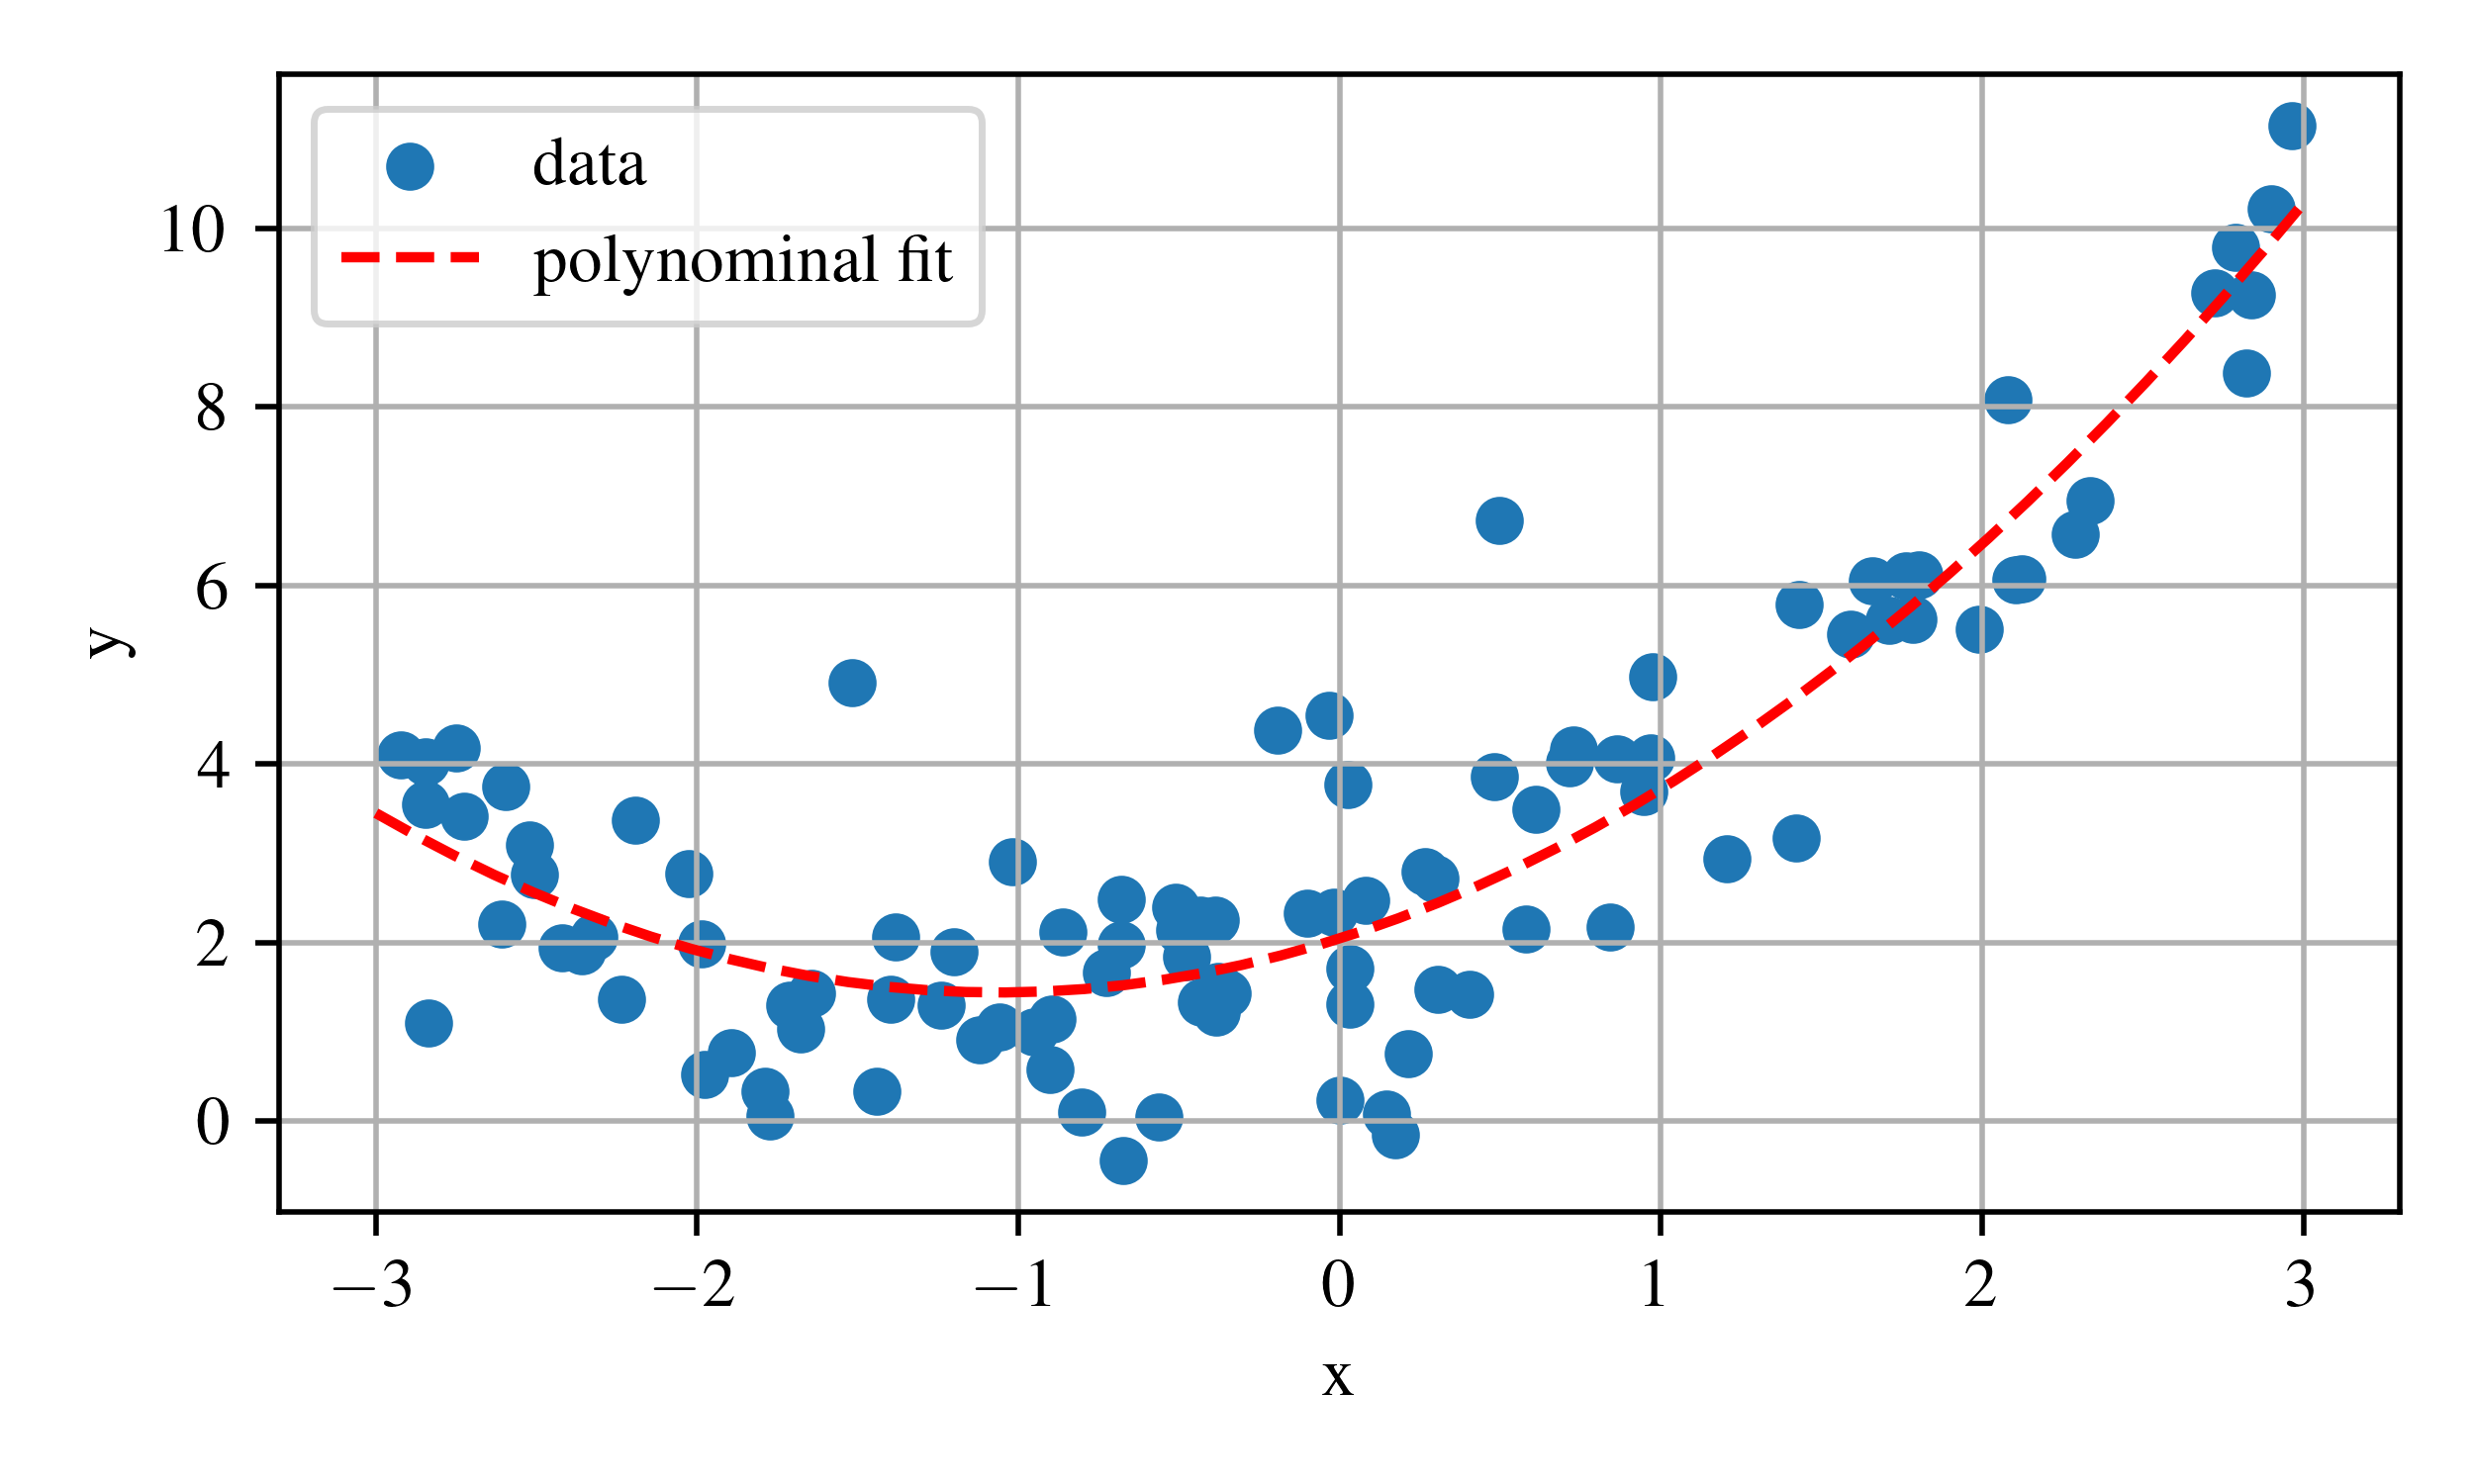
\includegraphics[width=4in]{../figures/polynomial_regression_3}
	\caption{Polynomial model fit via regression to a generic dataset. }
	\label{fig:general_regression}
\end{figure}
% \todo{need to update figure, add labels on x and y, get some sor of s-shaped data.}

In this chapter, we first examine Linear Regression and contrast two ways to estimate its parameters:
\begin{enumerate}
\item \textbf{Closed-form solution.} Solve for the parameter vector in one step by minimizing the cost function on the entire training set.  
\item \textbf{Gradient Descent .} Apply an iterative optimizer that repeatedly updates the parameters in small steps that lower the cost until it reaches the same optimum found by the closed-form method. We will look at three common Gradient Descent variants: Batch Gradient Descent, Mini-batch Gradient Descent, and Stochastic Gradient Descent.
\end{enumerate}
The first approach gives an exact answer immediately, whereas the second reaches that answer through successive refinements.




\pagebreak
\begin{data}

	\textbf{Ames Housing Dataset}

	\noindent The Ames housing dataset provides details on individual residential property sales in Ames, Iowa, from 2006 to 2010 \protect\footnotemark[1]. It includes 2,930 entries and numerous variables (23 nominal, 23 ordinal, 14 discrete, and 20 continuous) that are used to evaluate home values \protect\footnotemark[2].
	
	\footnotetext[1]{The author of this text bought a home in Ames Iowa during this time right as the 2008 housing crash unfolded and on the last day they allowed home loans with no down payment.}
	\footnotetext[2]{De Cock, Dean. ``Ames, Iowa: Alternative to the Boston housing data as an end of semester regression project.'' Journal of Statistics Education 19.3 (2011).}
	%\footnotetext[2]{De Cock, Dean. ``Ames, Iowa: Alternative to the Boston housing data as an end of semester regression project.'' Journal of Statistics Education 19.3 (2011).}
	
	\begin{figure}[H]
		\centering
		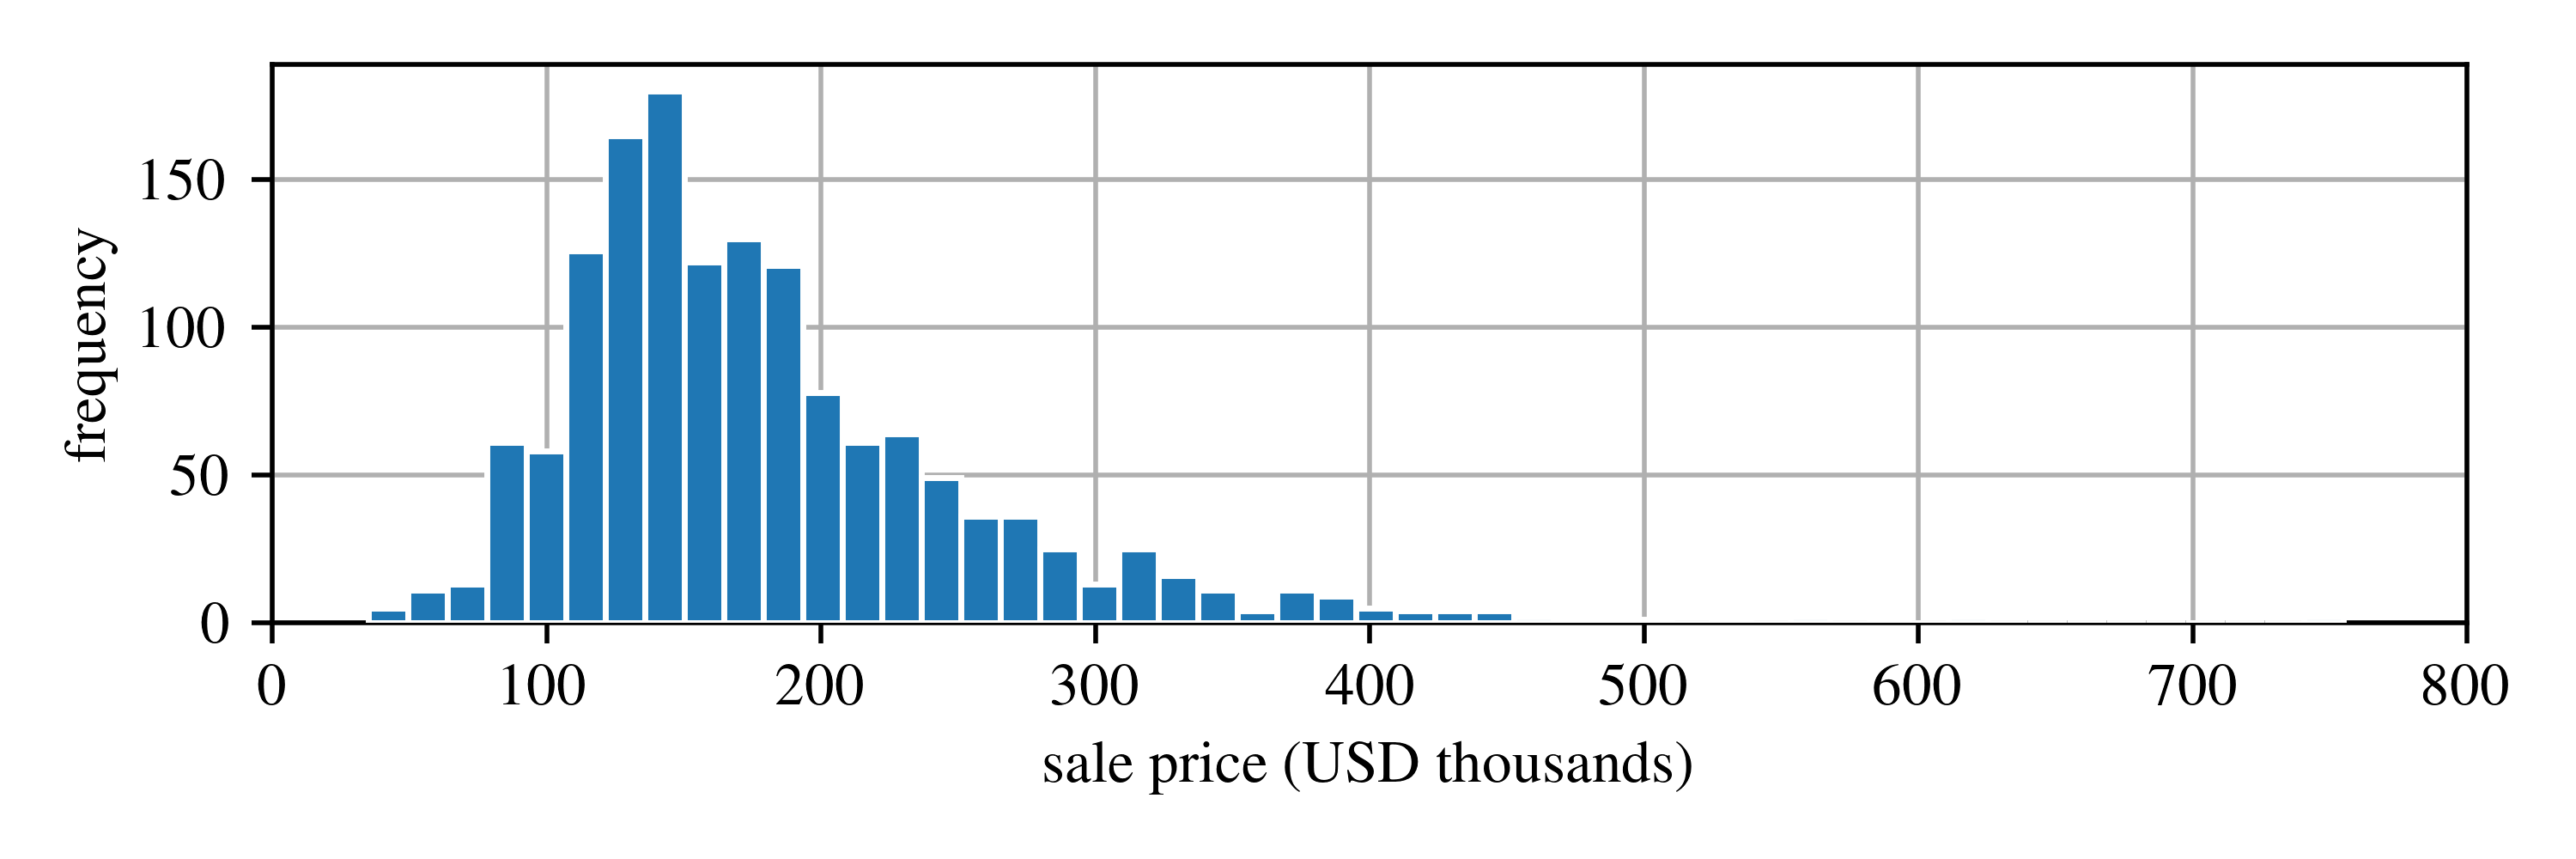
\includegraphics[width=5in]{../figures/Ames_histogram}
		\caption{Histogram of sale prices from 2006 to 2010 for the 2,930 entries.}
		\label{fig:Ames_histogram}
	\end{figure}
	
	\begin{figure}[H]
		\centering
		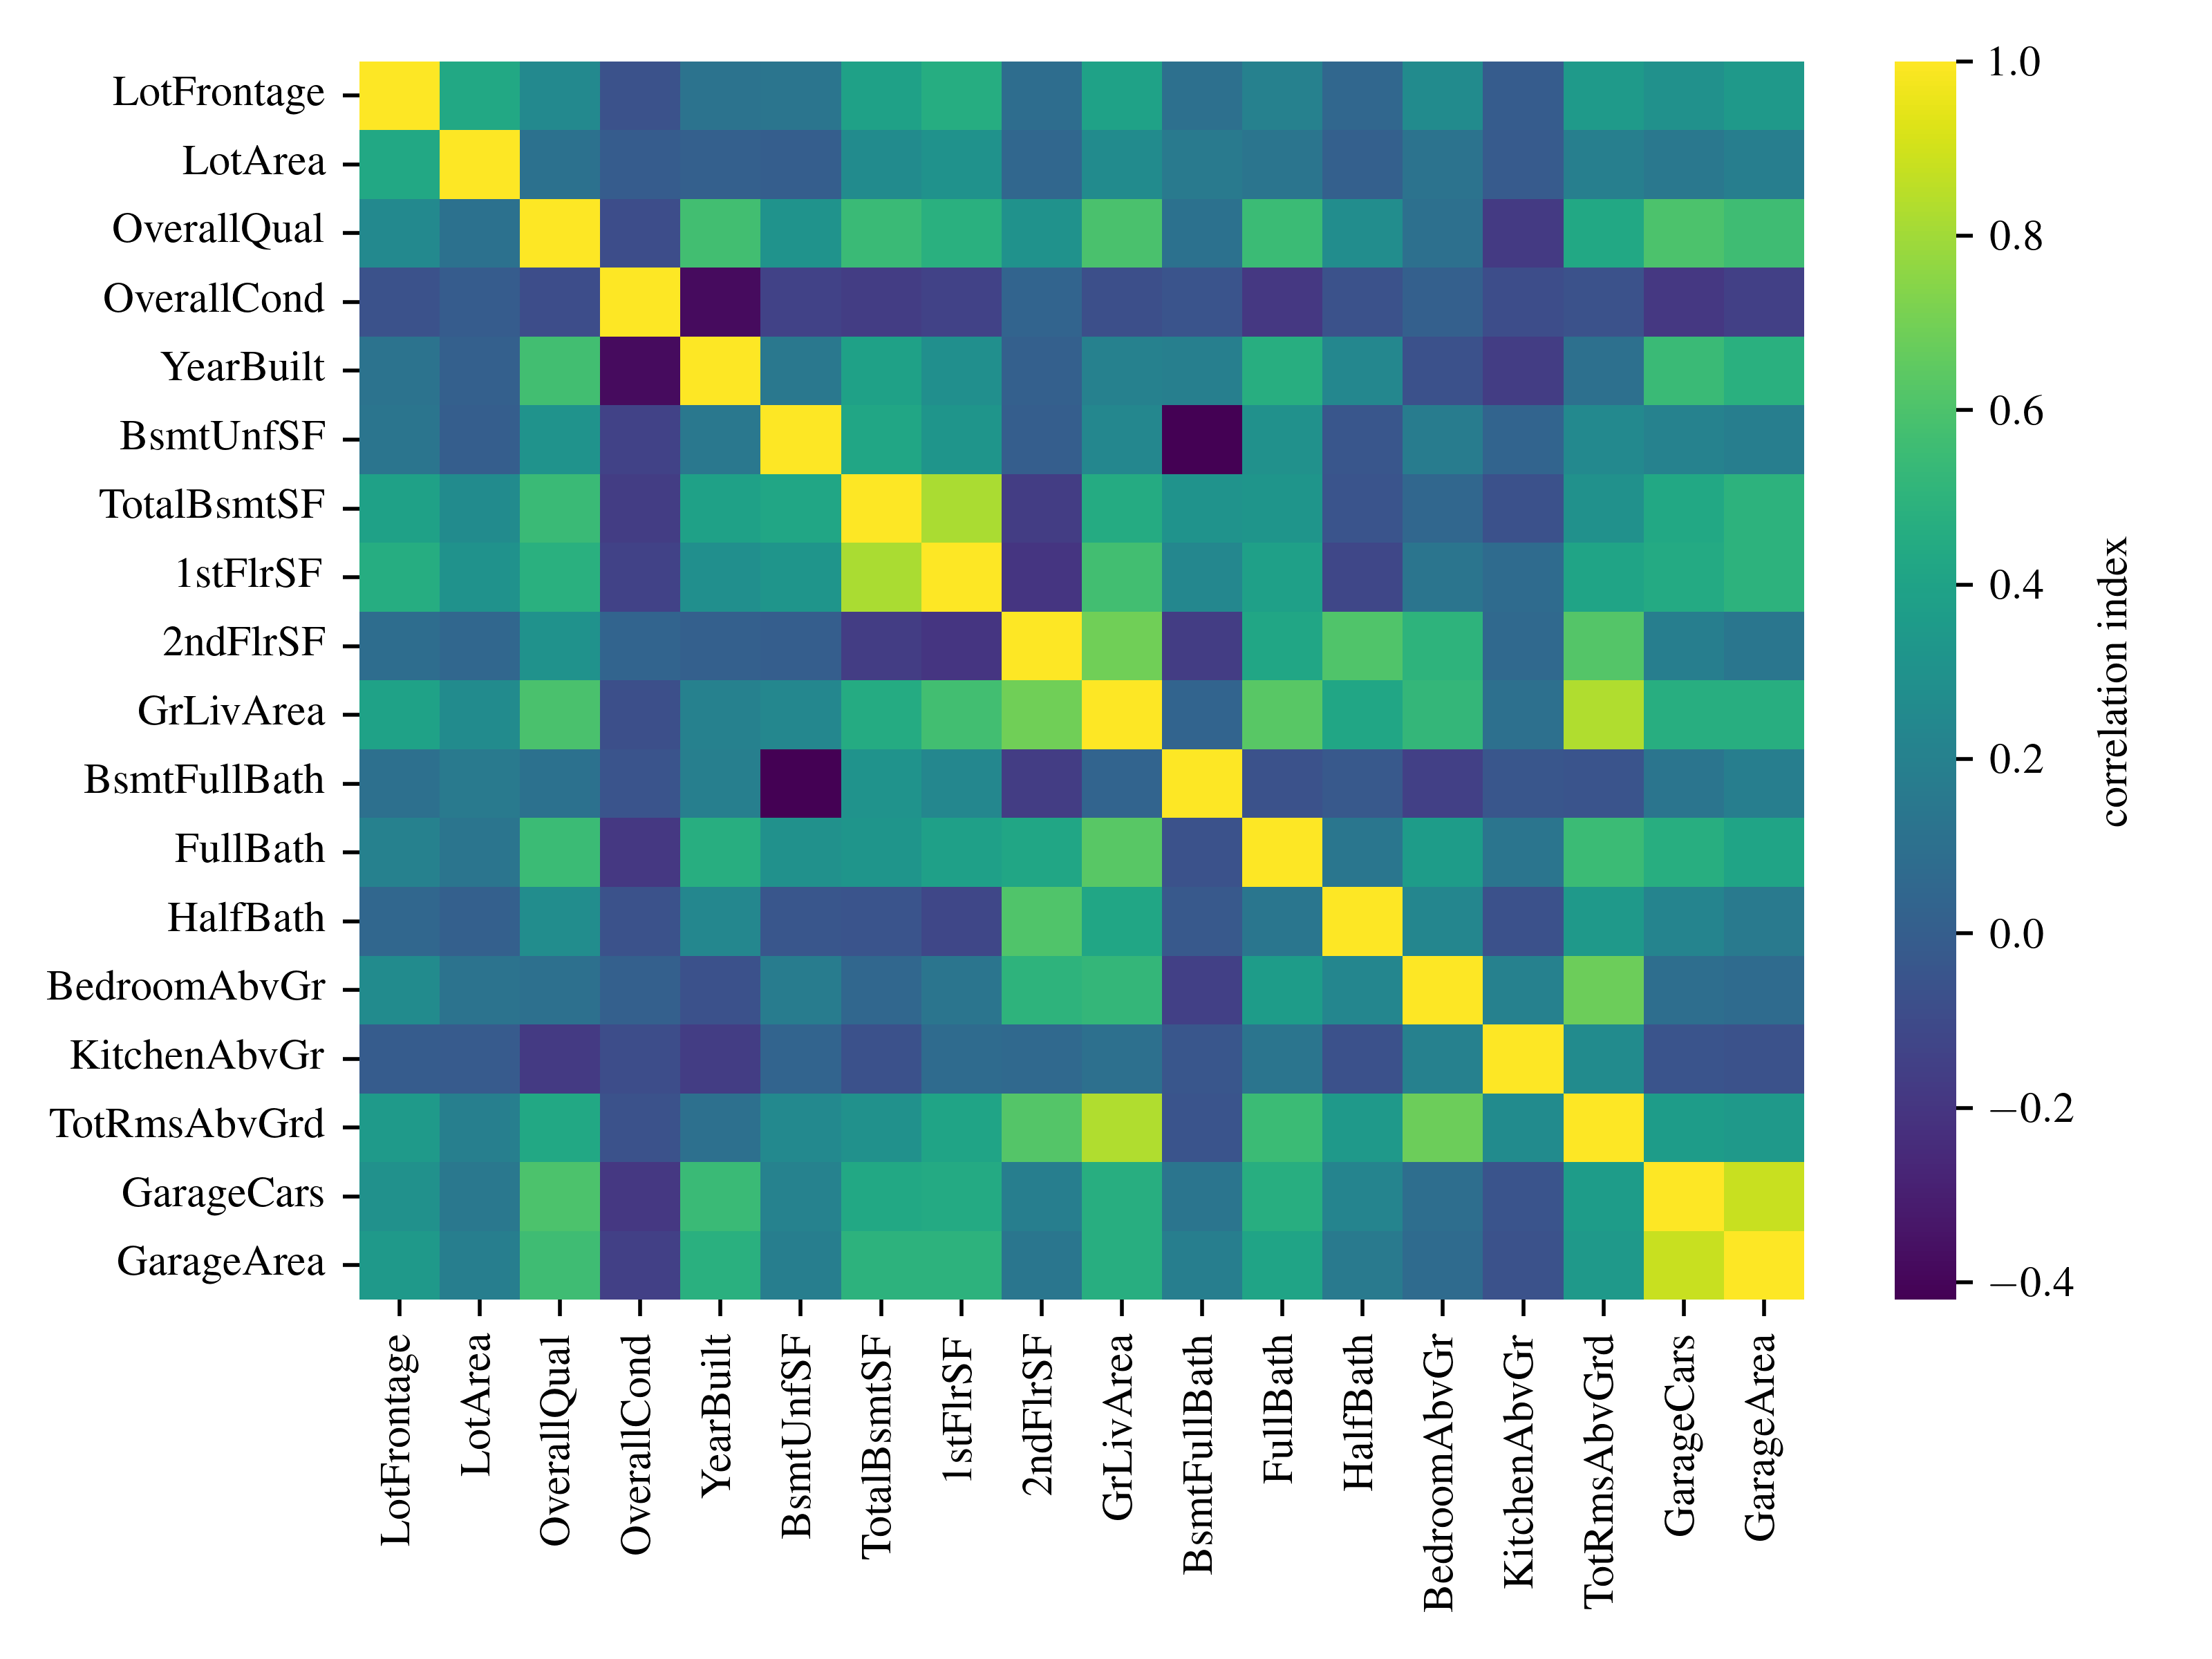
\includegraphics[width=5in]{../figures/Ames_housing_correlation_matirx}
		\caption{Correlation matrix for the 13 input parameters.}
		\label{fig:Ames_housing_correlation_matirx}
	\end{figure}

\end{data}



\pagebreak

\subsection{Linear Regression}
\vspace{-1ex}


Consider the scenario where you wish to determine the value of a house in Ames using the Ames dataset included in sklearn. To illustrate this, let us plot the relationship between the above ground living area and the housing price.

\begin{figure}[H]
    \centering
	\vspace{-1ex}
    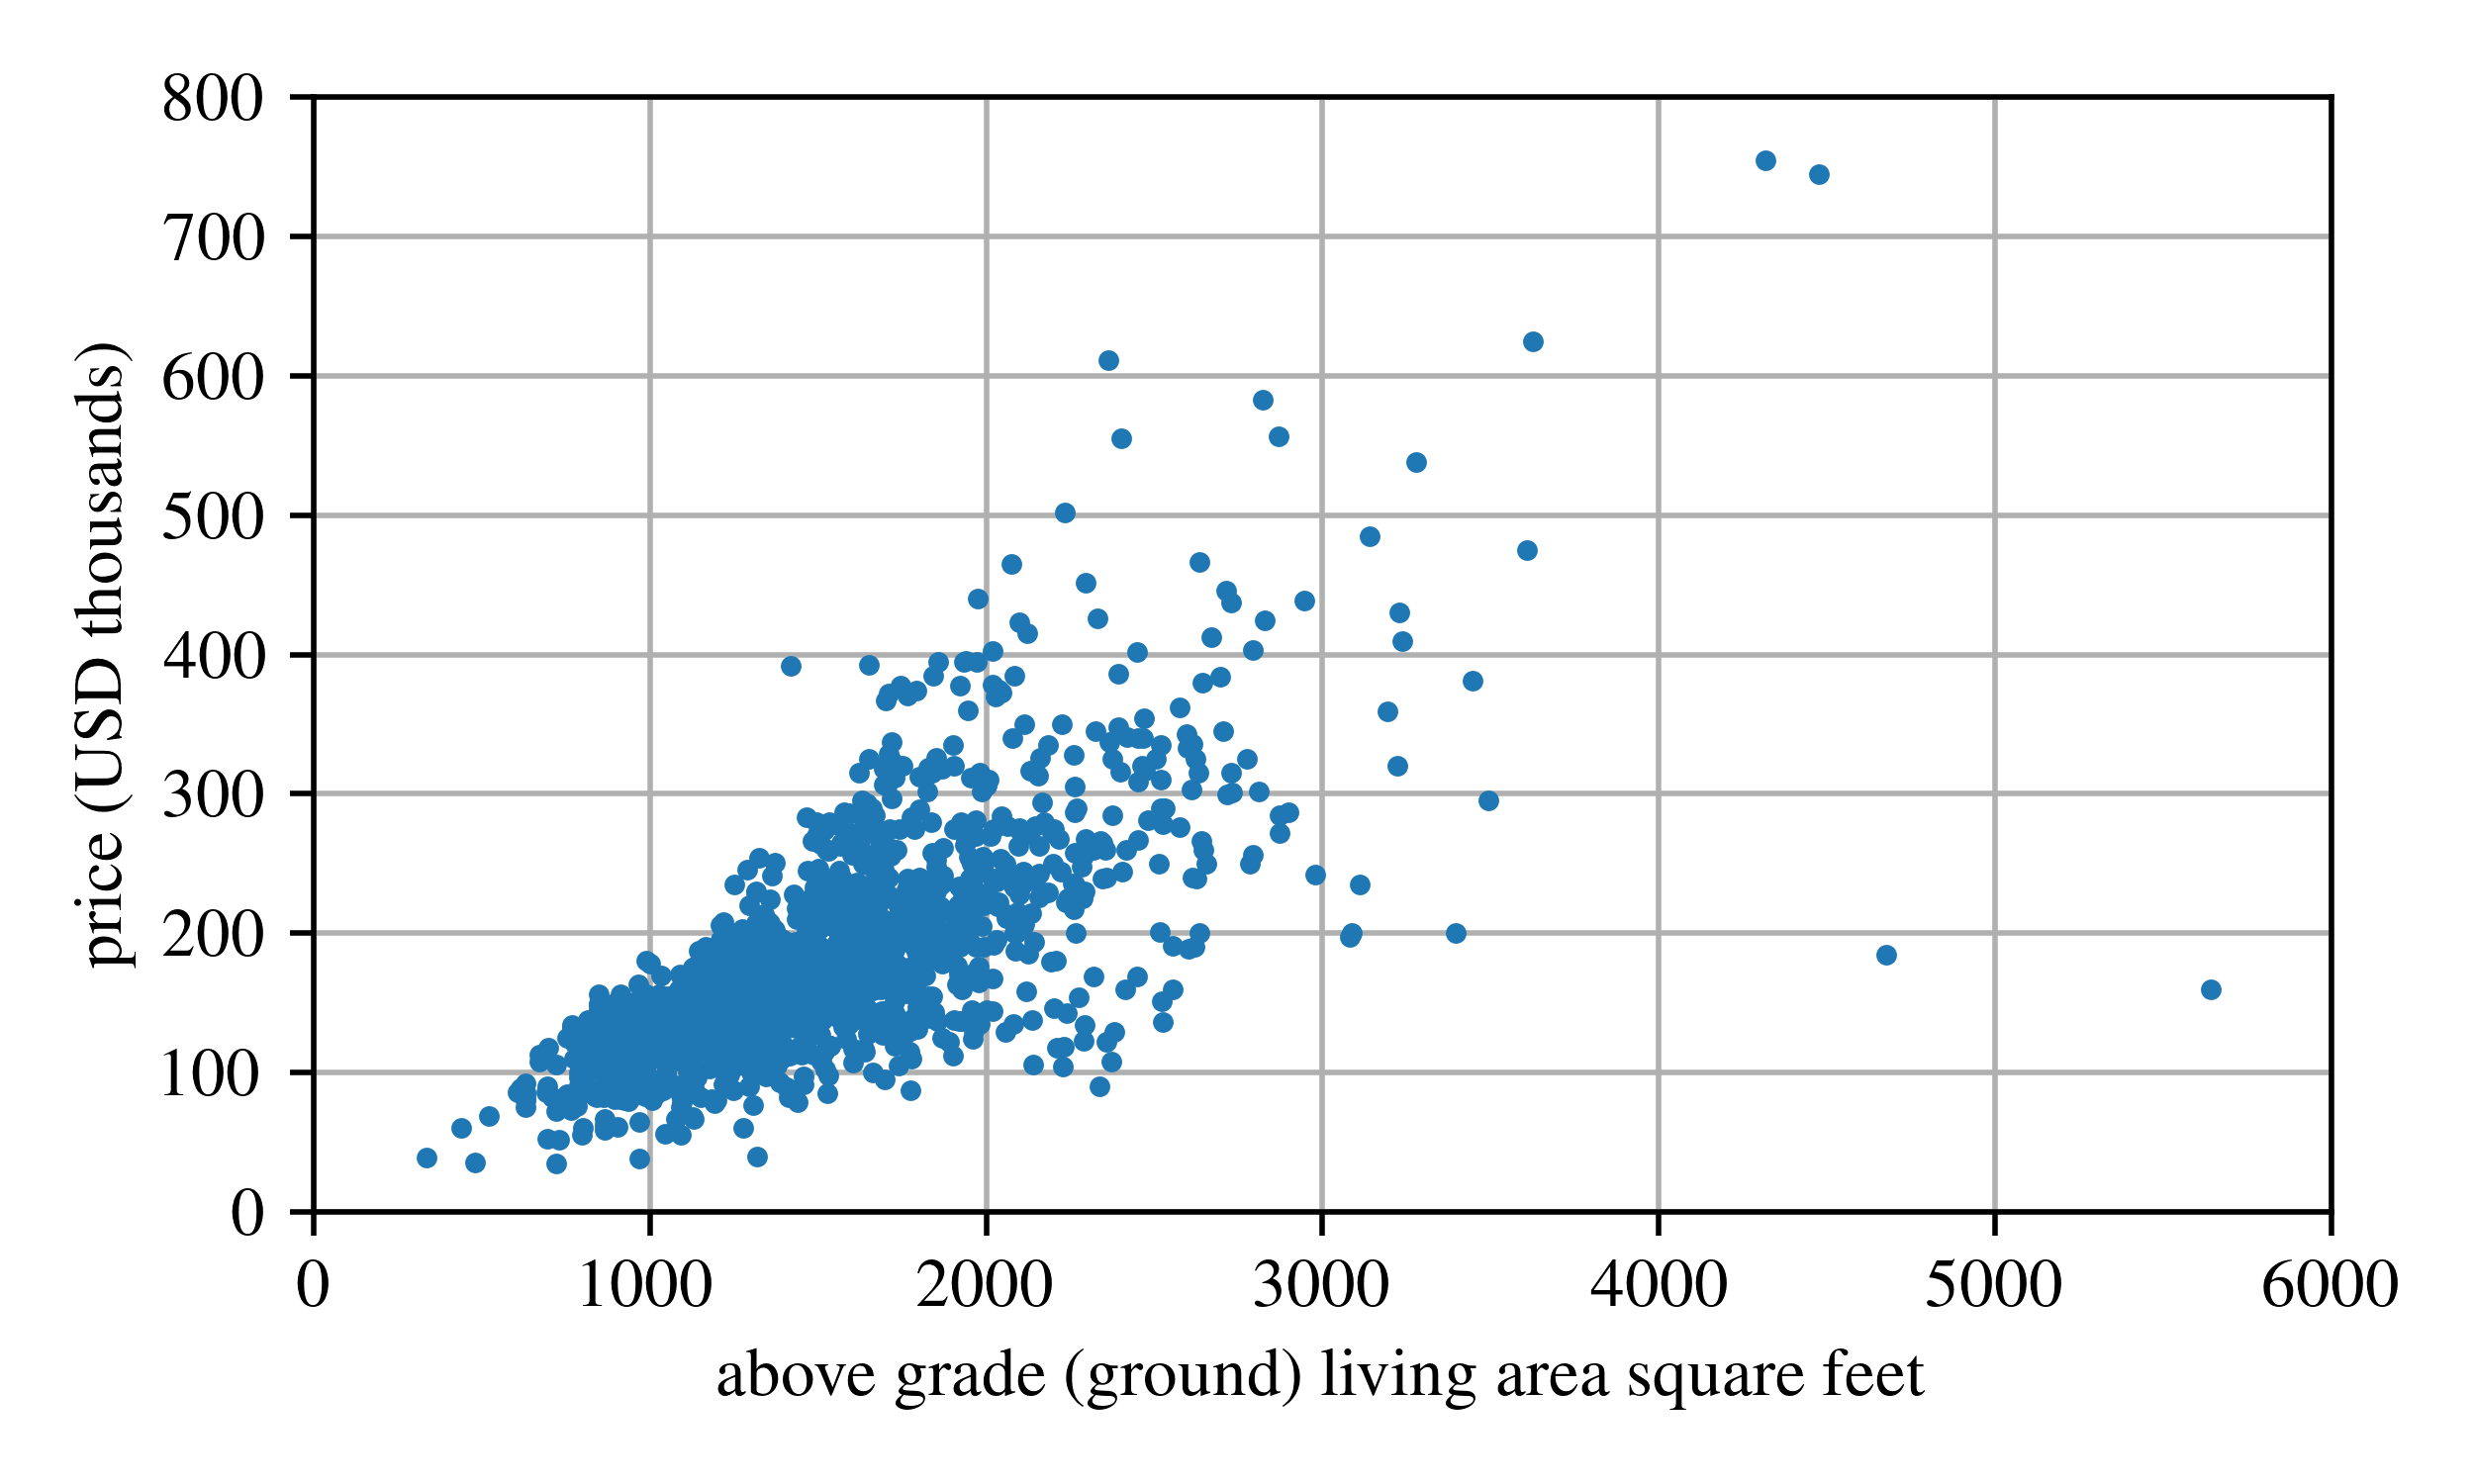
\includegraphics[]{../figures/Ames_simple_linear_regression_model_1.png}
	\vspace{-2ex}
    \caption{Ames housing data.}
    \label{fig:Ames_simple_linear_regression_model_1}
\end{figure}

A clear trend is observable, despite the data's noise (i.e., partial randomness): the value of a house increases with the above ground living area. Therefore, the house value can be modeled as a linear function of the above ground living area:
\begin{equation}
\text{price\_model} = \theta_1 + \theta_2 \times \text{above\_ground\_living\_area}
\end{equation}
This model comprises two parameters, $\theta_1$ and $\theta_2$, which can be adjusted to represent any linear relationship.

\begin{figure}[H]
    \centering
	\vspace{-1ex}
    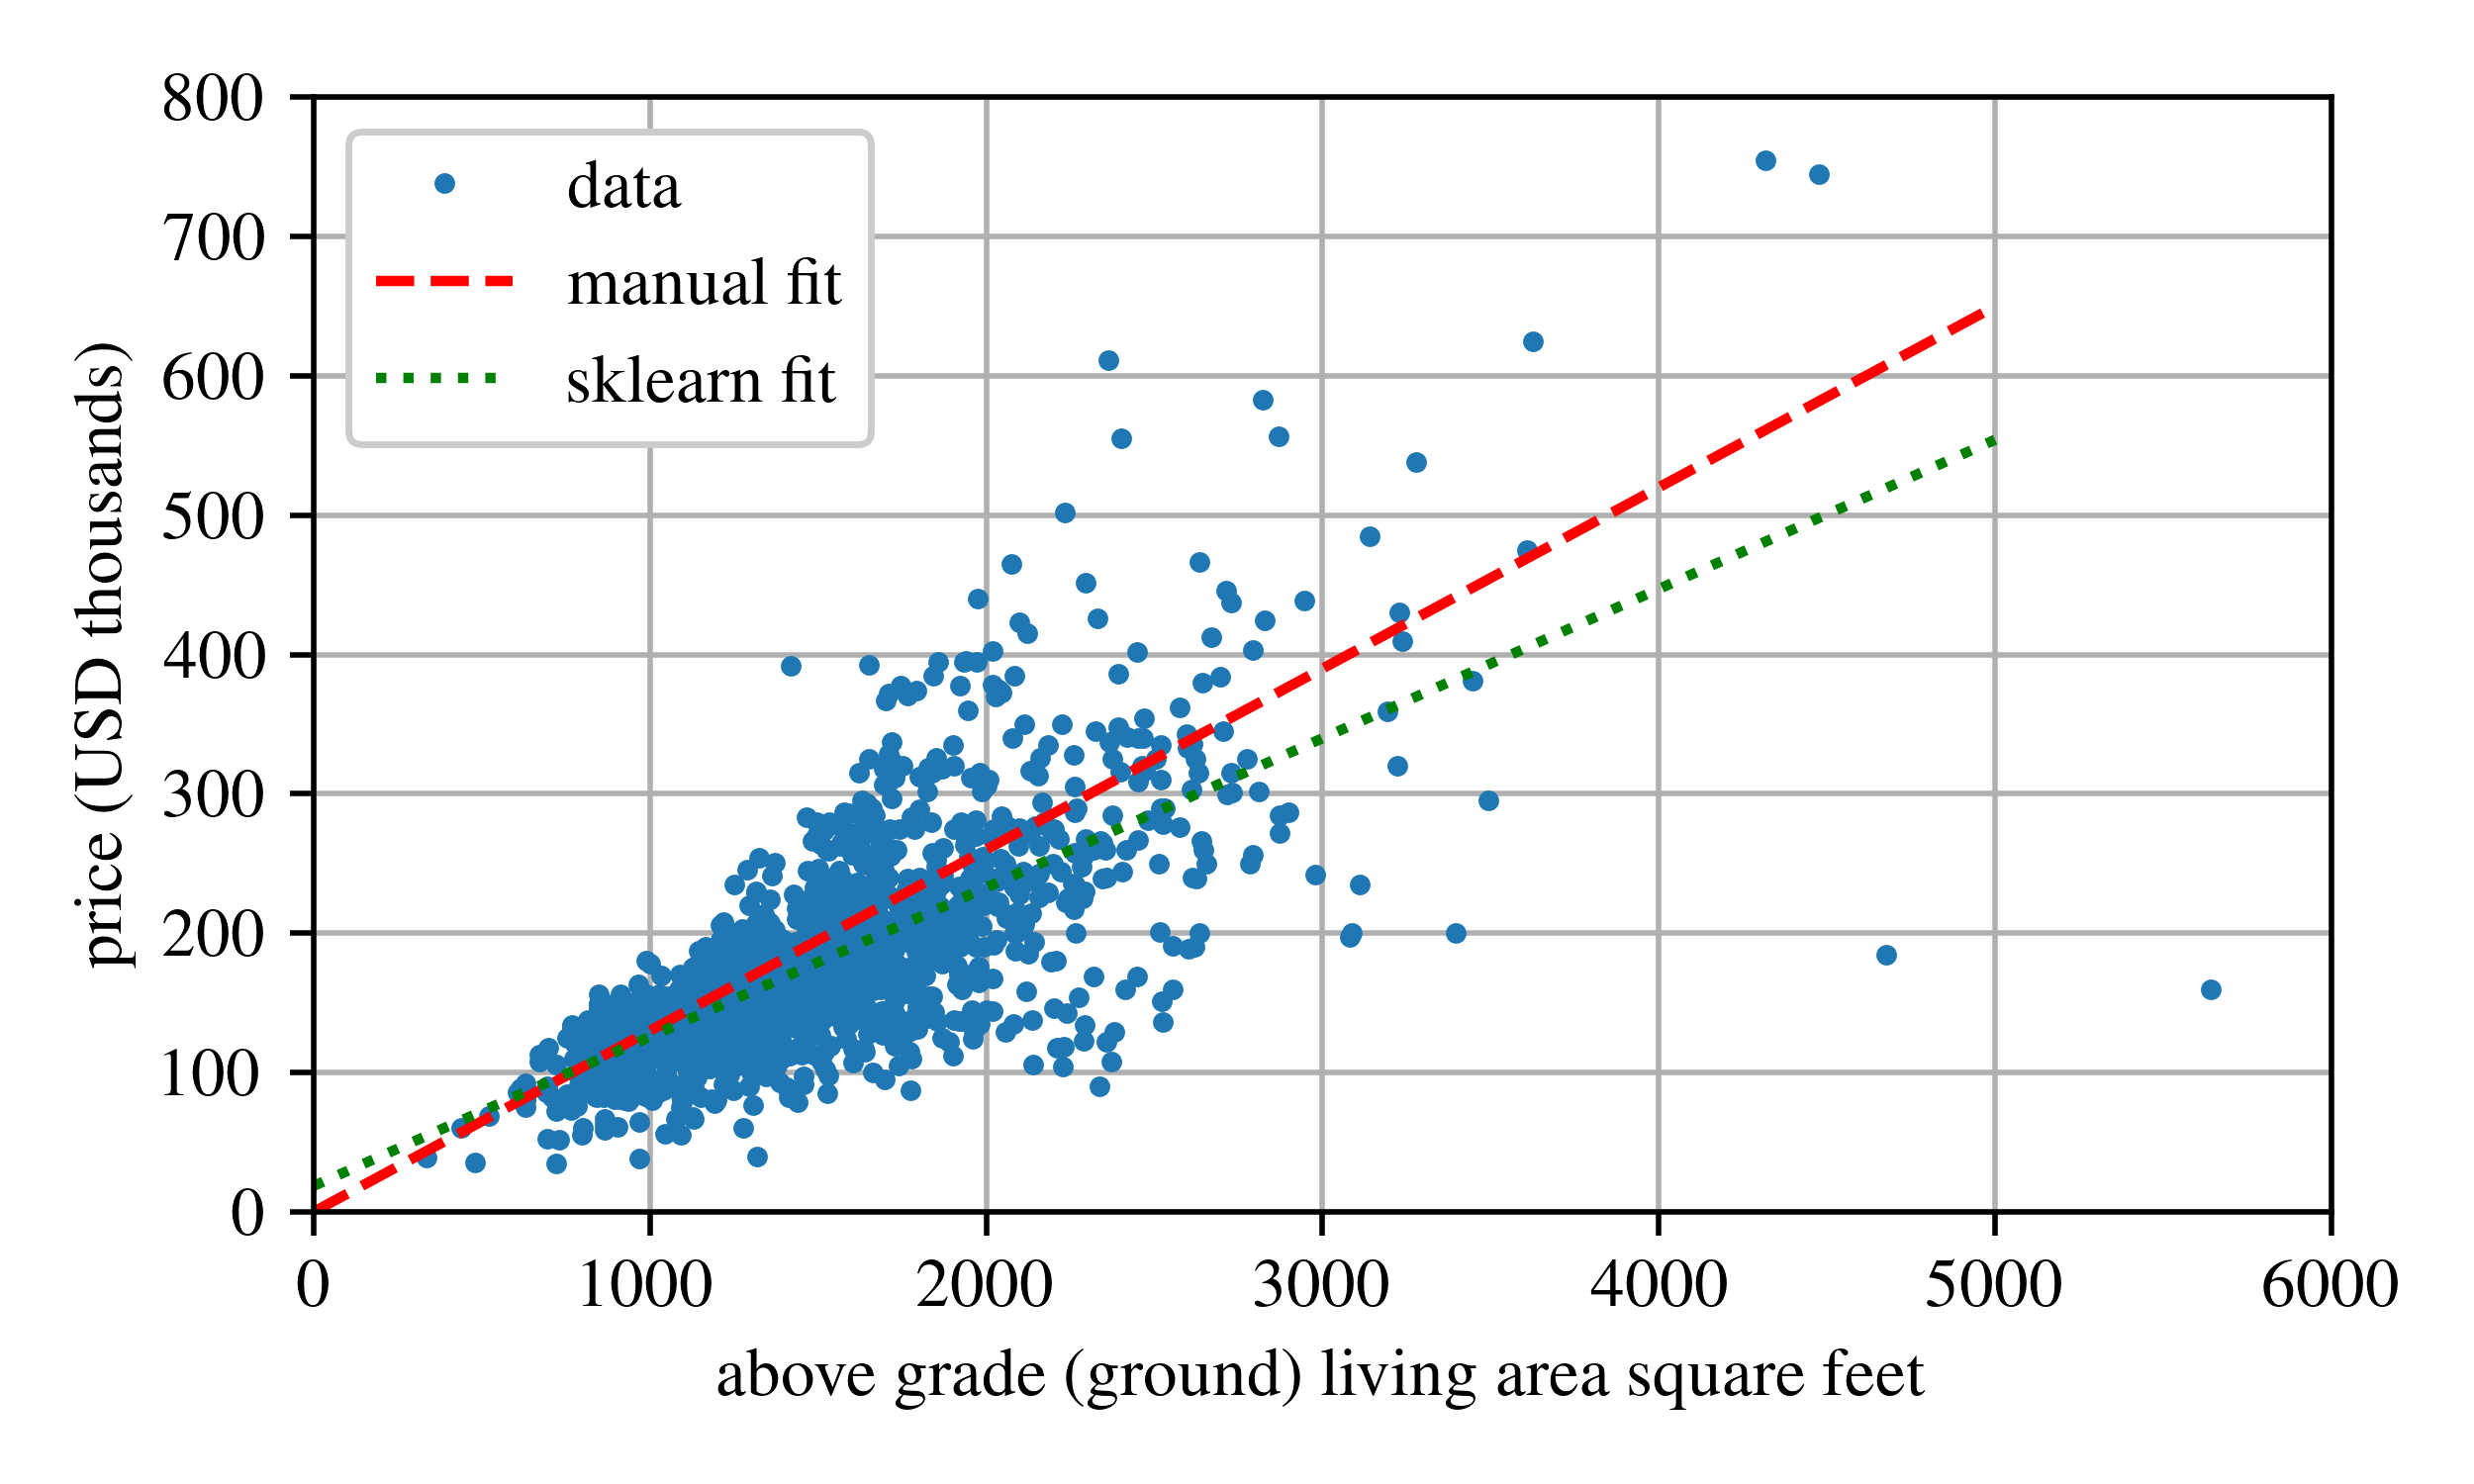
\includegraphics[]{../figures/Ames_simple_linear_regression_model_2.png}
	\vspace{-2ex}
    \caption{Ames housing data with trend lines.}
    \label{fig:GDP_data_trend}
\end{figure}






\pagebreak

\begin{mdframed}[middlelinewidth=0.5mm]
\begin{center}
\gr{Notations}
\end{center}

\begin{itemize}[itemsep=0.25ex]
    \item $\textbf{x}$: a lowercase, bolded variable that denotes a vector.
    \item $\textbf{X}$: an uppercase, bolded variable that represents a matrix.
    \item $\textbf{X}$: this denotes the feature matrix, also known as the input matrix.
    \item $\textbf{y}$: this is the label vector corresponding to the feature matrix, representing the target outputs.
    \item $\textbf{x}^{(i)}$ represents the $i^\text{th}$ instance in the dataset $\textbf{X}$. For instance, a dataset about cats might include an entry for a specific cat named Mittens. This entry (labelled $y$) could detail several attributes such as age, weight, and length.
    \item $h$: the hypothesis or prediction function that, given a feature vector $\textbf{X}$, outputs the predicted values $\hat{\textbf{y}} = h(\textbf{X})$.
    \item $n$: the total number of features in the dataset, which defines the complexity or degree of the model.
    \item $m$: the total number of instances in the dataset.
    \item $\hat{x}$: an estimated value, indicated by a hat, and pronounced as ``$x$-hat''.
\end{itemize}
\end{mdframed}

	\vspace{-2ex}
\subsubsection{Closed Form Solution}
	\vspace{-1ex}

Before you can tune a model's parameters, you need a clear way to judge how well it fits the data. The standard approach is to define a cost function that assigns a numerical penalty to poor fits; lower values indicate better performance. For a linear model, this cost function measures the difference between the model's predictions and the actual training targets, and you minimize that difference using Ordinary Least Squares linear regression. Practically, you feed your training data into the algorithm, which then solves for the parameter values that align the linear relationship most closely to the data. In Python, this procedure is implemented in \texttt{scikit-learn} as \texttt{sklearn.linear\_model.LinearRegression}.

%
%To determine the optimal parameter values that enhance your model's performance, it is essential to define a suitable performance measure. 
%\begin{itemize}
%    \item We establish a cost function to quantify the inadequacy of the fit, where a lower value indicates a better fit.
%    \item For a linear model, we utilize a cost function that calculates the discrepancy between the model's predictions and the actual training data. The goal is to minimize this discrepancy, commonly addressed in Ordinary Least Squares Linear Regression.
%    \begin{itemize}
%        \item This involves inputting your training data into the algorithm, which then determines the parameters that best align the linear model with your data.
%        \item The function is implemented in scikit-learn as ``sklearn.linear\_model.LinearRegression''.
%    \end{itemize}
%\end{itemize}

In the context of the Ames housing data, a straightforward cost function used is the Mean Squared Error (MSE), defined as
\begin{equation}
\text{MSE} = J = \frac{1}{m} \sum_{i=1}^{m} (\hat{y}_i-y_i)^2
\end{equation}
\noindent where $m$ is the number of dataset instances, and $J$ serves as a general representation of the cost function in machine learning contexts.

The MSE is also applied to minimize the error in a linear regression model, with the hypothesis $h_\theta$, trained on dataset $\textbf{X}$. This is expressed as:
\begin{equation}
\text{MSE}(\textbf{X},h_\theta) = J = \frac{1}{m} \sum_{i=1}^{m} (\pmb{\theta}^\text{T}\textbf{x}^{(i)}-y^{(i)})^2
\end{equation}
\noindent where the objective is to minimize the cost function by iteratively refining the values of $\pmb{\theta}$.

\begin{figure}[H]
    \centering
    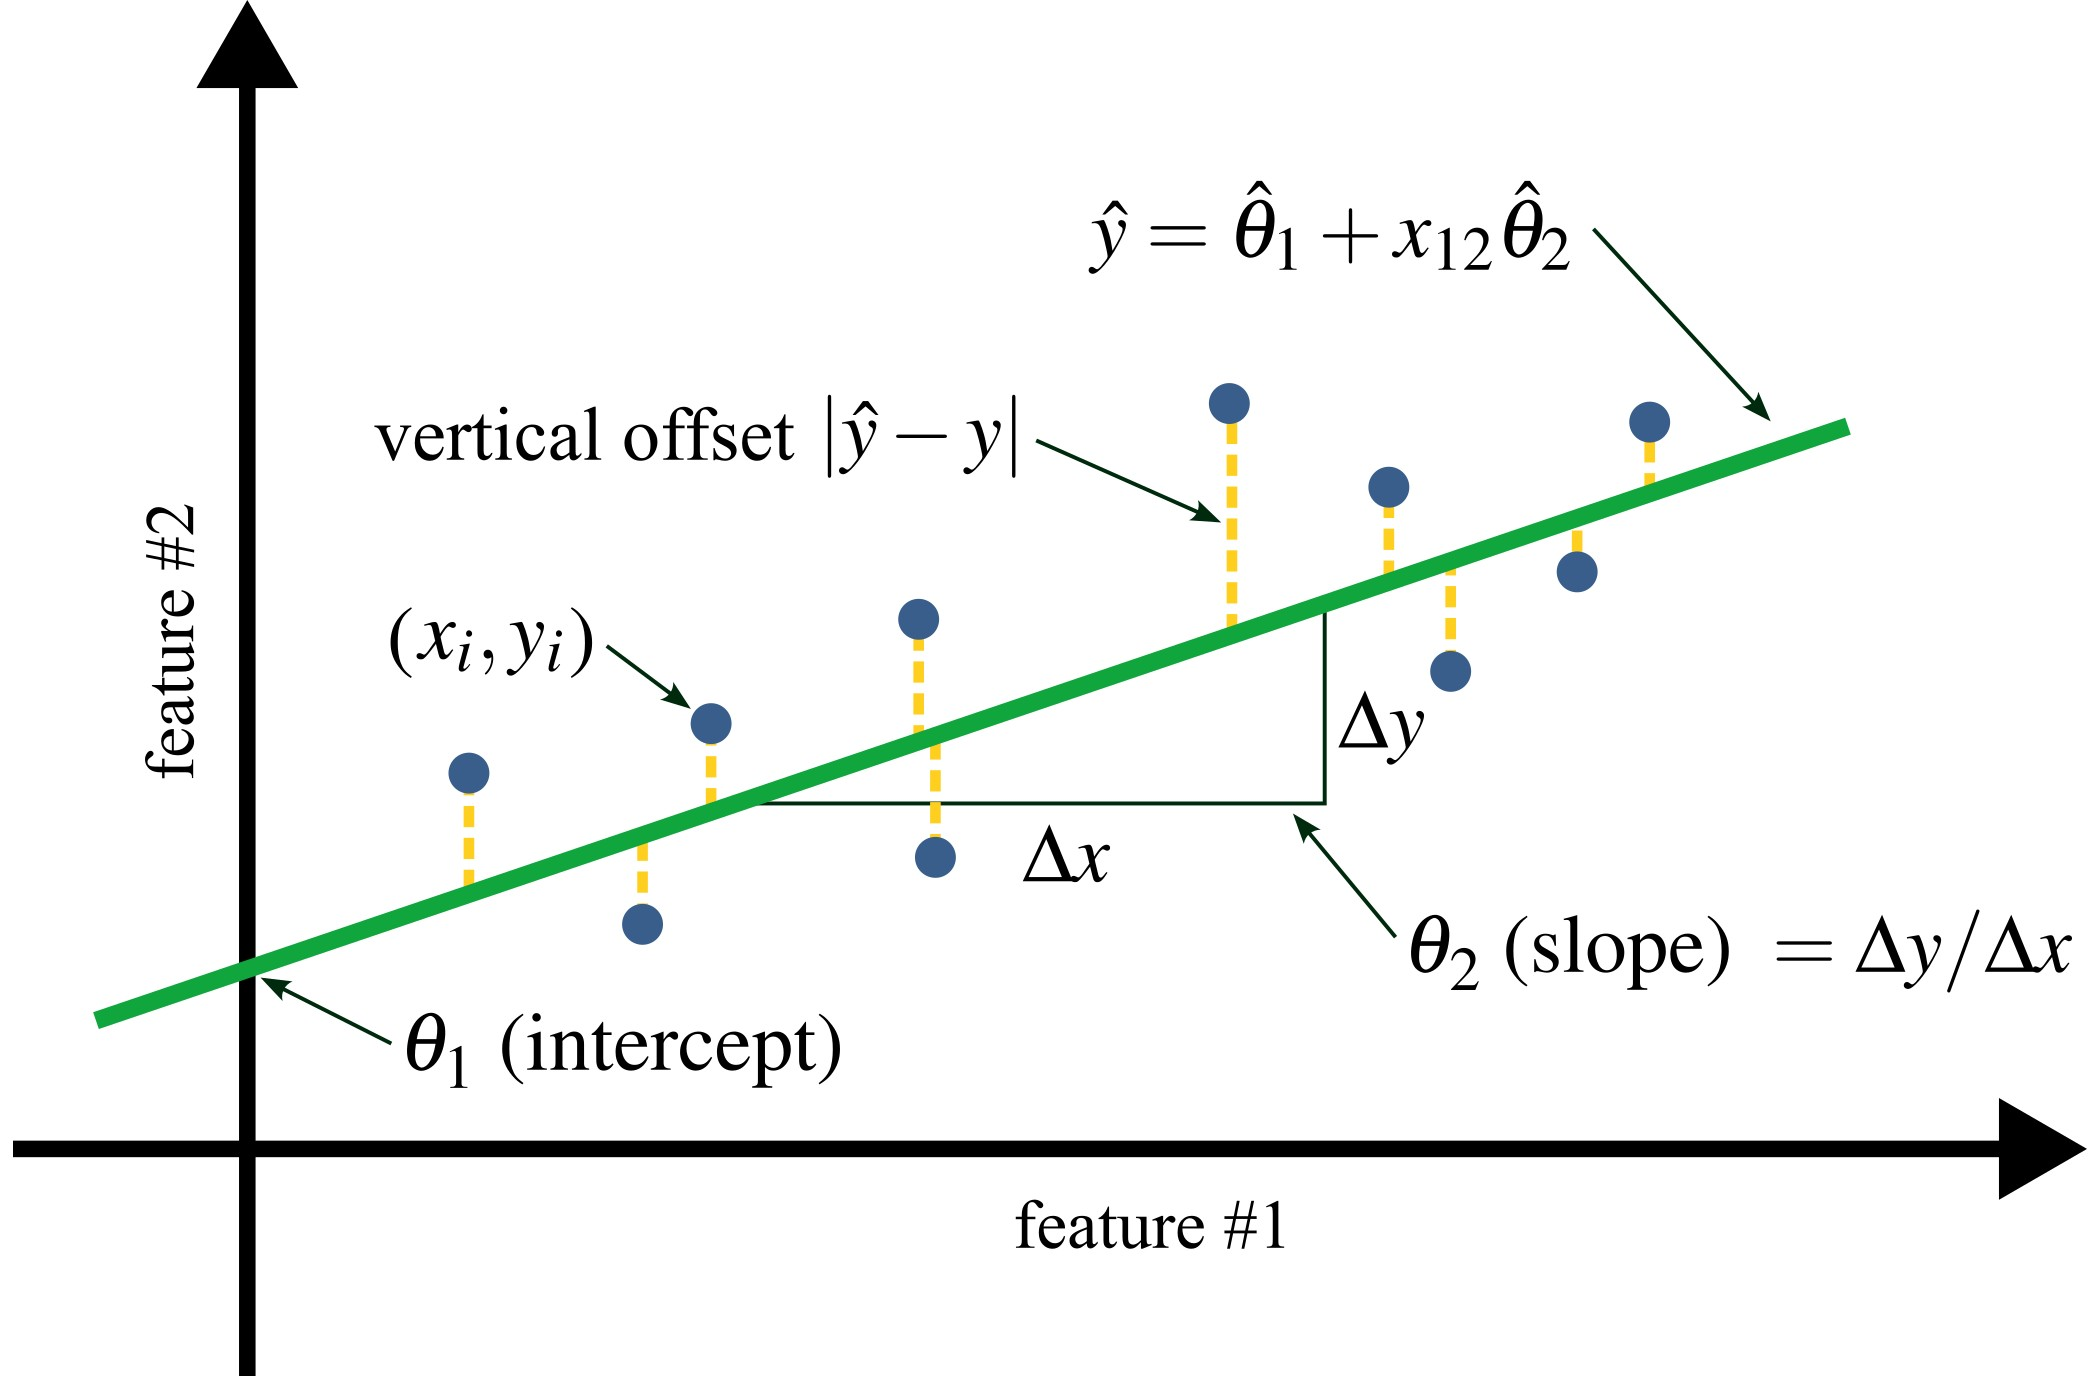
\includegraphics[width=4.2in]{../figures/least_squares}
    \caption{Linear regression of a two-feature dataset obtained with least squares.}
    \label{fig:least_squares}
\end{figure}

%% Math for the figure above
%$|\hat{y}-y|$ \\
%$x_i,y_i$ \\
%$\Delta x$ \\
%$\Delta y$ \\
%$\theta_1 \text{ (intercept)}$\\
%$\theta_2 \text{ (slope) } = \Delta y / \Delta x$ \\
%$\hat{y} = \hat{\theta}_1 + x_{12}\hat{\theta}_2$ \\

Consider a dataset containing $n$ observations, denoted as $(y_i, x_i)^n_{i=1}$. Each observation $i$ consists of a scalar response $y_i$ and a column vector $x_i$ that holds the values for $p$ predictors (regressors), represented as $x_{ij}$ where $j = 1, \dots, p$. In the context of a linear regression model, the response variable $y_i$ is modeled as a linear combination of the regressors, influenced by an error term $\epsilon_i$:
\begin{equation}
 y_i = \theta_1x_{i1}+\theta_2x_{i2}+\hdots+\theta_yx_{im}+\epsilon_i 
\end{equation}
This model can also be written in matrix notation as
\begin{equation}
\textbf{y} = \textbf{X} \pmb{\theta} + \epsilon
\end{equation}
Where: 
\begin{equation}
	\textbf{X} = \begin{bmatrix}
	x_{11} & x_{12} & \hdots & x_{1m} \\
	x_{21} & x_{22} & \hdots & x_{2m} \\
	\vdots & \vdots & \ddots & \vdots \\
	x_{n1} & x_{n2} & \hdots & x_{nm}
	\end{bmatrix},\;
	\pmb{\theta} = \begin{bmatrix}
	\theta_1 \\
	\theta_2 \\
	\vdots \\
	\theta_p
	\end{bmatrix},\;
	\textbf{y}=\begin{bmatrix}
	y_1 \\
	y_2 \\
	\vdots \\
	y_n
	\end{bmatrix}
\end{equation}
However, the best-fit model $\hat{y}$ will not be able to account for the unmodeled error, therefore: 
\begin{equation}
 \hat{y}_i = \hat{\theta}_1x_{i1}+\hat{\theta}_2x_{i2}+\hdots+\hat{\theta}_m x_{im}
\end{equation}
or 
\begin{equation}
 \hat{\textbf{y}} = \textbf{X} \hat{\pmb{\theta}}
\end{equation}


This goal is to find $\hat{\theta}$ such that the error is minimized. Mathmatically, this is simple enough as the $\hat{\theta}$ Is the minimization of the lease-squares hyperplane, or:
\begin{equation}
\hat{\pmb{\theta}}=(\textbf{X}\textsuperscript{T}\textbf{X})^{-1}\textbf{X}\textsuperscript{T}\textbf{y}
\label{eq:normal_equation}
\end{equation}
Equation~\ref{eq:normal_equation} is referred to as the normal equation. Consider a simple linear model with $p = 2$, where $x_{11} = 1$. In this scenario, $x_{11}$ acts as the bias term of the equation, whereas the remaining elements of $\textbf{X}$ represent the data. Without this bias term, the solution would only address the slope of the line. Subsequently, solving for $\hat{\theta}_1$ and $\hat{\theta}_2$ yields:
\begin{equation}
 [x_{11}x_{12}][\hat{\theta}_1\hat{\theta}_2] = \hat{y}
\end{equation}
As $x_{11} = 1$ (again, called the bias term) this becomes:
\begin{equation}
 \hat{y} = \hat{\theta}_1 + x_{12}\hat{\theta}_2
\end{equation}
This is simply another expression for the equation of a liner line:
\begin{equation}
y = mx + b
\end{equation}
Solving the model output for a input or a series of inputs can than be done simply enough. 

\begin{figure}[H]
	\centering
	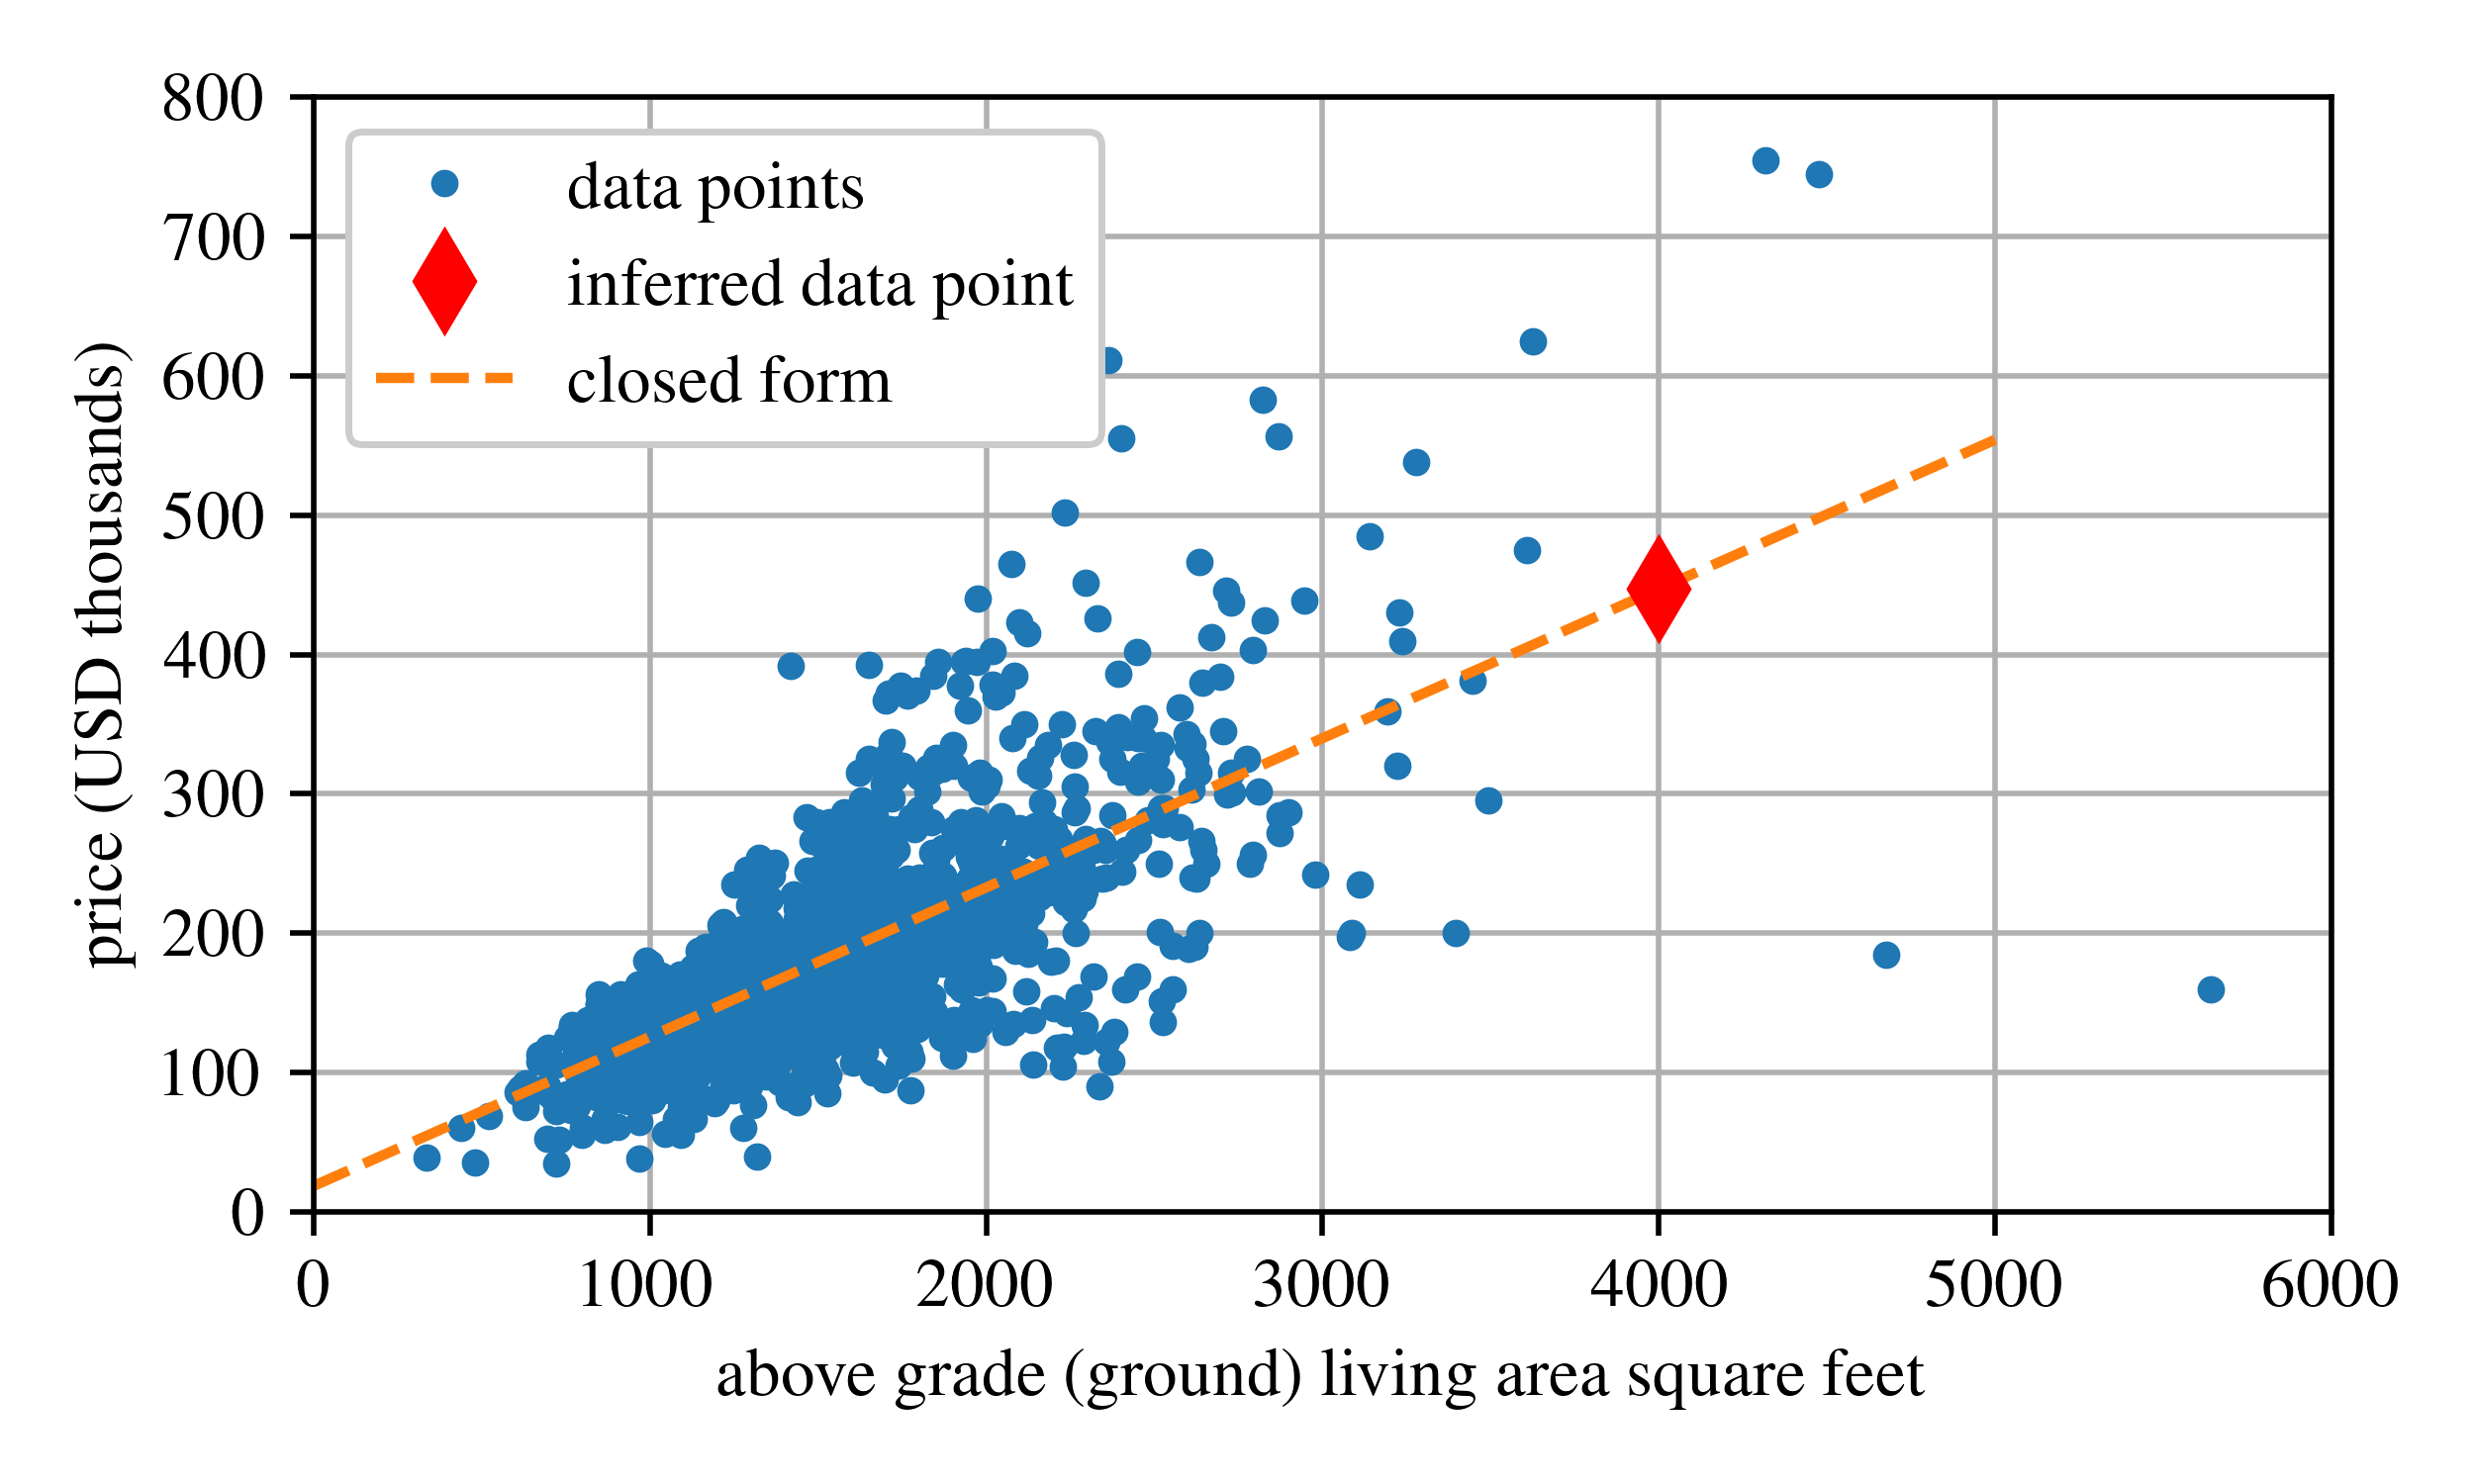
\includegraphics[]{../figures/Ames_simple_linear_regression_model_3.png}
	\caption{Ames housing data inferred.}
	\label{fig:Ames_simple_linear_regression_model_3}
\end{figure}


\subsubsection{Computational Complexity}

The Normal Equation calculates the inverse of $\textbf{X}^\text{T}\textbf{X}$, an $n \times n$ matrix, where $n$ represents the number of features. The computational complexity of matrix inversion generally ranges from $O(n^{2.4})$ to $O(n^3)$, depending on the specific algorithm used. Consequently, doubling the number of features would increase the computational effort by approximately $2^{2.4} \approx 5.3$ to $2^3 = 8$ times.


\begin{mdframed}[middlelinewidth=0.5mm]
\begin{center}
\rd{WARNING}
\end{center}
When the number of features becomes very large, for example around $100,000$, solving the Normal Equation becomes extremely slow.
\end{mdframed}



On the positive side, the computational complexity of this equation is linear with respect to the number of instances in the training set, denoted as $O(m)$. This allows it to efficiently handle large training sets, as long as they fit within memory.

Furthermore, once your Linear Regression model is trained (whether through the Normal Equation or another method), making predictions is very quick. The computational effort is linear in relation to both the number of instances you wish to predict and the number of features. Essentially, predicting for twice as many instances or features will approximately double the computation time.

Next, we will explore different methods for training a Linear Regression model that are more appropriate for scenarios with a large number of features, or when the training data exceeds memory capacity.

\begin{example}
\textbf{Linear Regression - Ames Housing Dataset}

\noindent This example uses the Ames housing dataset to model the relationship between above-ground living area and house price using linear regression. It compares a manual fit, a closed-form solution, and gradient descent, alongside Scikit-Learn's \texttt{LinearRegression} and \texttt{SGDRegressor}, to illustrate how each method fits a line to the data.

\end{example}

%\lstset{%
%caption={Example functions for Python code.},
%label={lst:functions},
%language=Python,
%basicstyle=\ttm,
%morekeywords={self},              % Add keywords here
%keywordstyle=\ttb\color{deepblue},
%emph={MyClass,__init__},          % Custom highlighting
%emphstyle=\ttb\color{deepred},    % Custom highlighting style
%stringstyle=\color{deepgreen},
%frame=tb,                         % Any extra options here
%showstringspaces=false
%}
%\begin{lstlisting}
%i=20
%
%class MyClass(Yourclass):
%    def __init__(self, my, yours):
%        bla = '5 1 2 3 4'
%        print bla
%
%# this is a comment
%for i in range(10):
%	i=10
%
%
%
%\end{lstlisting}


Gradient Descent is a versatile optimization algorithm capable of finding optimal solutions across a broad spectrum of problems. The core concept of Gradient Descent involves iteratively adjusting parameters to minimize a cost function \protect\footnotemark[1]. Consider the analogy of being lost in a dense fog in the mountains and seeking to descend:
\begin{enumerate}
\item You sense the ground's slope under your feet (the local gradient).
\item You descend in the direction of the steepest descent.
\item Reaching a point where the local gradient is zero indicates that you have found a minimum.
\end{enumerate}
	
\footnotetext[1]{Ruder, Sebastian. ``An overview of gradient descent optimization algorithms.'' arXiv preprint arXiv:1609.04747 (2016).}


The Gradient Descent process starts with random initialization of the parameter $\theta$, followed by gradual improvements. Each incremental step aims to reduce the cost function until the algorithm converges to a minimum.

\begin{figure}[H]
    \centering
    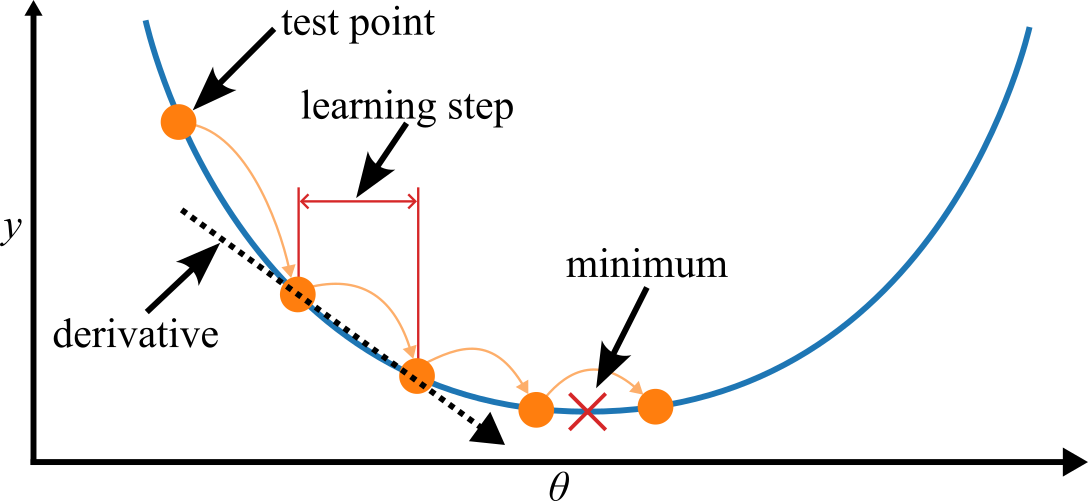
\includegraphics[]{../figures/gradient_descent_1}
    \caption{Illustration of gradient descent.}
    \label{fig:gradient_descent_1}
\end{figure}

A critical aspect of Gradient Descent is the step size, controlled by the learning rate hyperparameter. A small learning rate leads to a slow convergence, requiring many iterations. Conversely, a high learning rate might cause the algorithm to overshoot the minimum, potentially causing divergence and failing to find an optimal solution.

\begin{figure}[H]
    \centering
    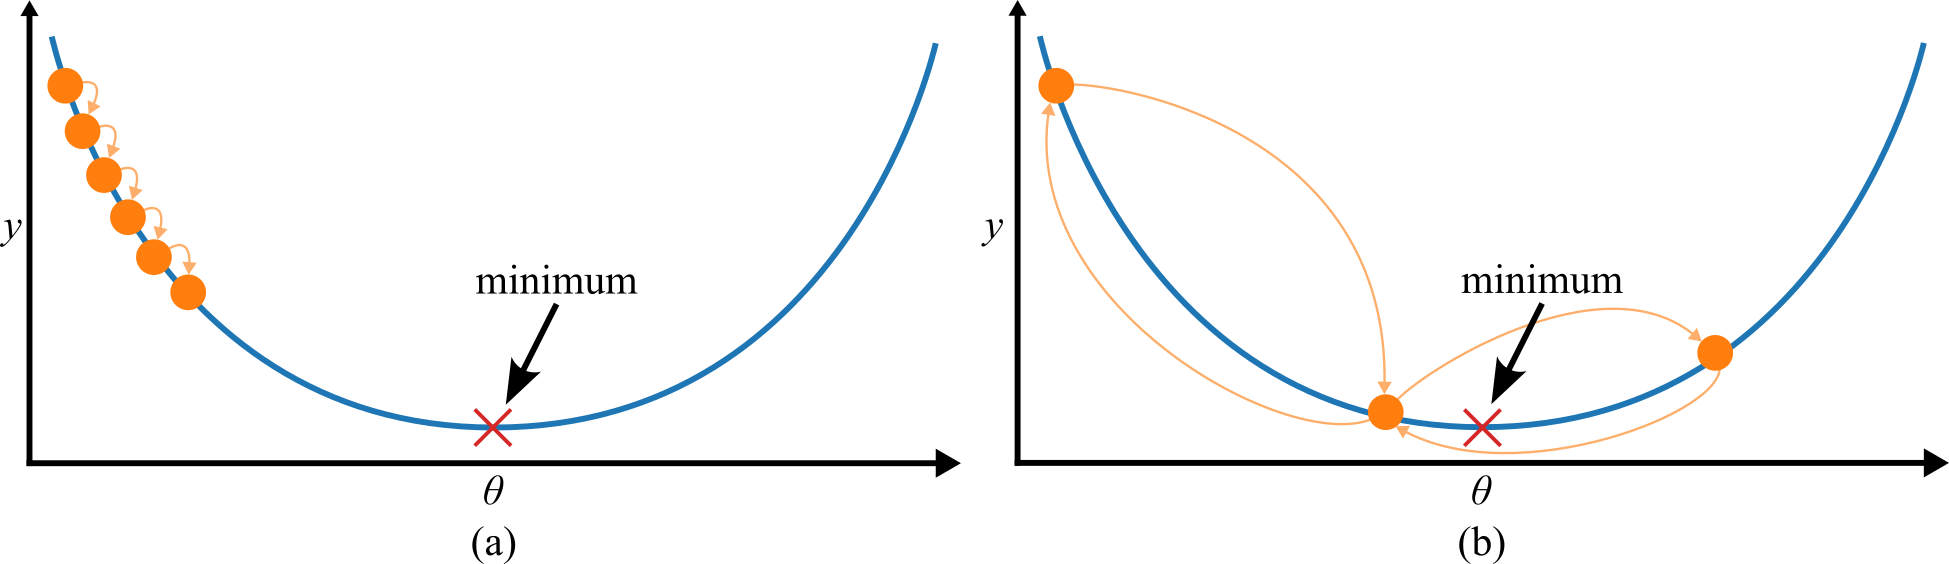
\includegraphics[]{../figures/gradient_descent_2}
    \caption{Effect of learning rate in gradient descent, showing: (a) a slow search with a low step size, and (b) a search with a large step size that oscillates around the minimum without ever finding the minimum.}
    \label{fig:gradient_descent_2}
\end{figure}



Cost functions do not always present themselves as neat, concave shapes. They can feature obstacles such as holes, ridges, plateaus, and various complex topographies that complicate the convergence to the minimum. The challenges associated with Gradient Descent include:
\begin{itemize}
\item Starting the algorithm from a random point on the left may lead to convergence at a local minimum rather than the more optimal global minimum.
\item Initiating on the right might result in a prolonged journey across a plateau, and terminating the process too soon could prevent reaching the global minimum.
\end{itemize}

\begin{figure}[H]
    \centering
    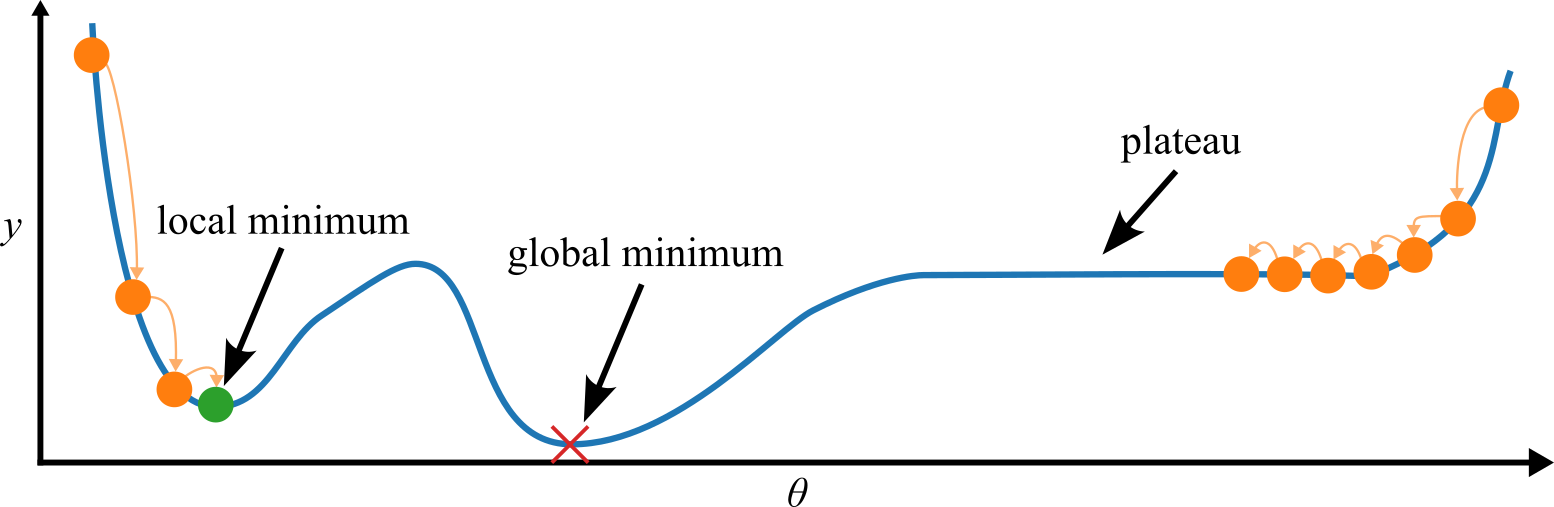
\includegraphics[]{../figures/gradient_descent_3}
    \caption{Gradient features and descent challenges.}
    \label{fig:gradient_descent_3}
\end{figure}


Fortunately, the Mean Squared Error (MSE) cost function for Linear Regression models is convex. This characteristic ensures that for any two points on the curve, the line segment joining them does not intersect the curve itself. Consequently:
\begin{itemize}
\item There are no local minima, only one global minimum exists.
\item It is a continuous function, and its slope changes smoothly.
\end{itemize}

These properties significantly benefit the optimization process: Gradient Descent can reliably approximate the global minimum given sufficient time and an appropriate learning rate.






\subsubsection{Comparison of Gradient Descent Methods}

Before looking into the mathematical details, let us examine how various gradient descent methods achieve the optimal solution, as illustrated in Figure~\ref{fig:Comparing_gradient_descent_methods}. Additionally, Table~\ref{table:Comparison_linear_regression} provides a comparative analysis of different gradient descent methods, highlighting their respective strengths and weaknesses.


\begin{figure}[H]
	\centering
	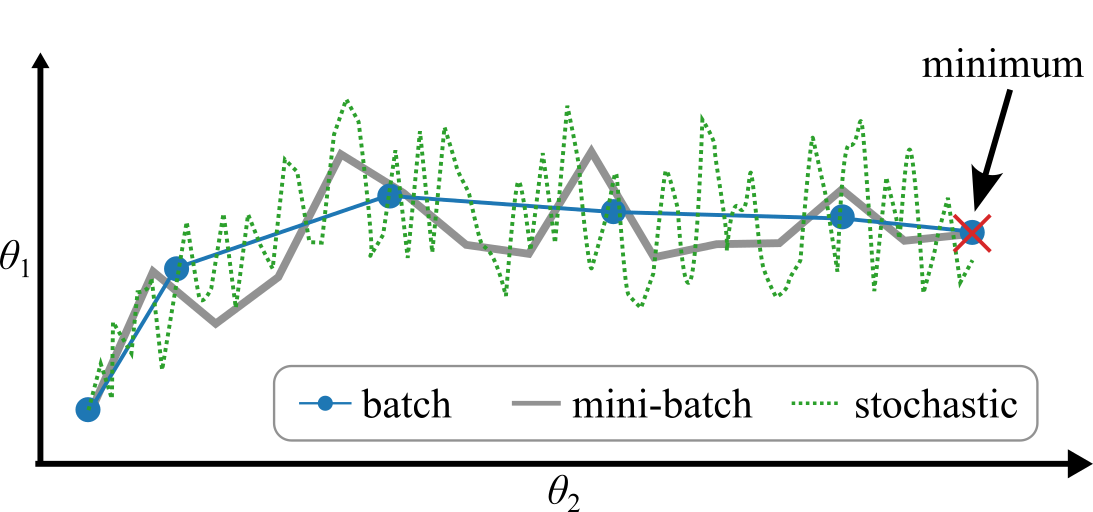
\includegraphics[]{../figures/comparing_gradient_descent_methods}
	\caption{Comparing gradient descent methods.}
	\label{fig:Comparing_gradient_descent_methods}
\end{figure}



% Please add the following required packages to your document preamble:
% \usepackage{booktabs}
\begin{table}[H]
\caption{Comparison of various linear regression solutions.}
\label{table:Comparison_linear_regression}
\resizebox{\textwidth}{!}{\begin{tabular}{@{}lllllll@{}}
\toprule
\multicolumn{1}{c}{algorithm} & {\begin{tabular}[c]{@{}c@{}}large number of\\  instances ($m$) \end{tabular}} & \multicolumn{1}{c}{\begin{tabular}[c]{@{}c@{}}data must\\ fit in memory\end{tabular}} & {\begin{tabular}[c]{@{}c@{}}large number of\\  features ($n$) \end{tabular}} & \multicolumn{1}{c}{hyperparams} & \multicolumn{1}{c}{\begin{tabular}[c]{@{}c@{}}scaling\\ required\end{tabular}} & \multicolumn{1}{c}{Scikit-Learn} \\ \midrule
normal equation & fast & yes & slow & 0 & no & \texttt{LinearRegression} \\
batch GD & slow & yes & fast & 2 & yes & n/a \\
stochastic GD & fast & no & fast &  $\ge 2$ & yes & \texttt{SGDRegressor} \\
mini-batch GD & fast & no & fast &  $\ge 2$ & yes & n/a \\ \bottomrule
\end{tabular}}
\end{table}




\begin{mdframed}[middlelinewidth=0.5mm]
\begin{center}
\bl{NOTE}
\end{center}
After training, there is minimal difference between the models: these algorithms converge on similar solutions and make predictions in a nearly identical manner.
\end{mdframed}






\subsubsection{Batch Gradient Descent}






Batch Gradient Descent (shown in figure~\ref{fig:gradient_descent_batch}) processes the entire batch of training data $\textbf{X}$ at every step, which is the origin of its name, ``batch.'' Consider again our Mean Squared Error (MSE) cost function:
\begin{equation}
J = \frac{1}{m} \sum_{i=1}^{m} (\hat{y}_i - y_i)^2
\end{equation}
For a hypothesis $h_\theta$, the MSE for the dataset $\textbf{X}$ can be computed for each instance $\textbf{x}^{(i)}$ as follows:
\begin{equation}
J(\textbf{X}, h_\theta) = J = \frac{1}{m} \sum_{i=1}^{m} (\pmb{\theta}^\text{T}\textbf{x}^{(i)} - y^{(i)})^2
\end{equation}

\begin{figure}[h]
	\centering
	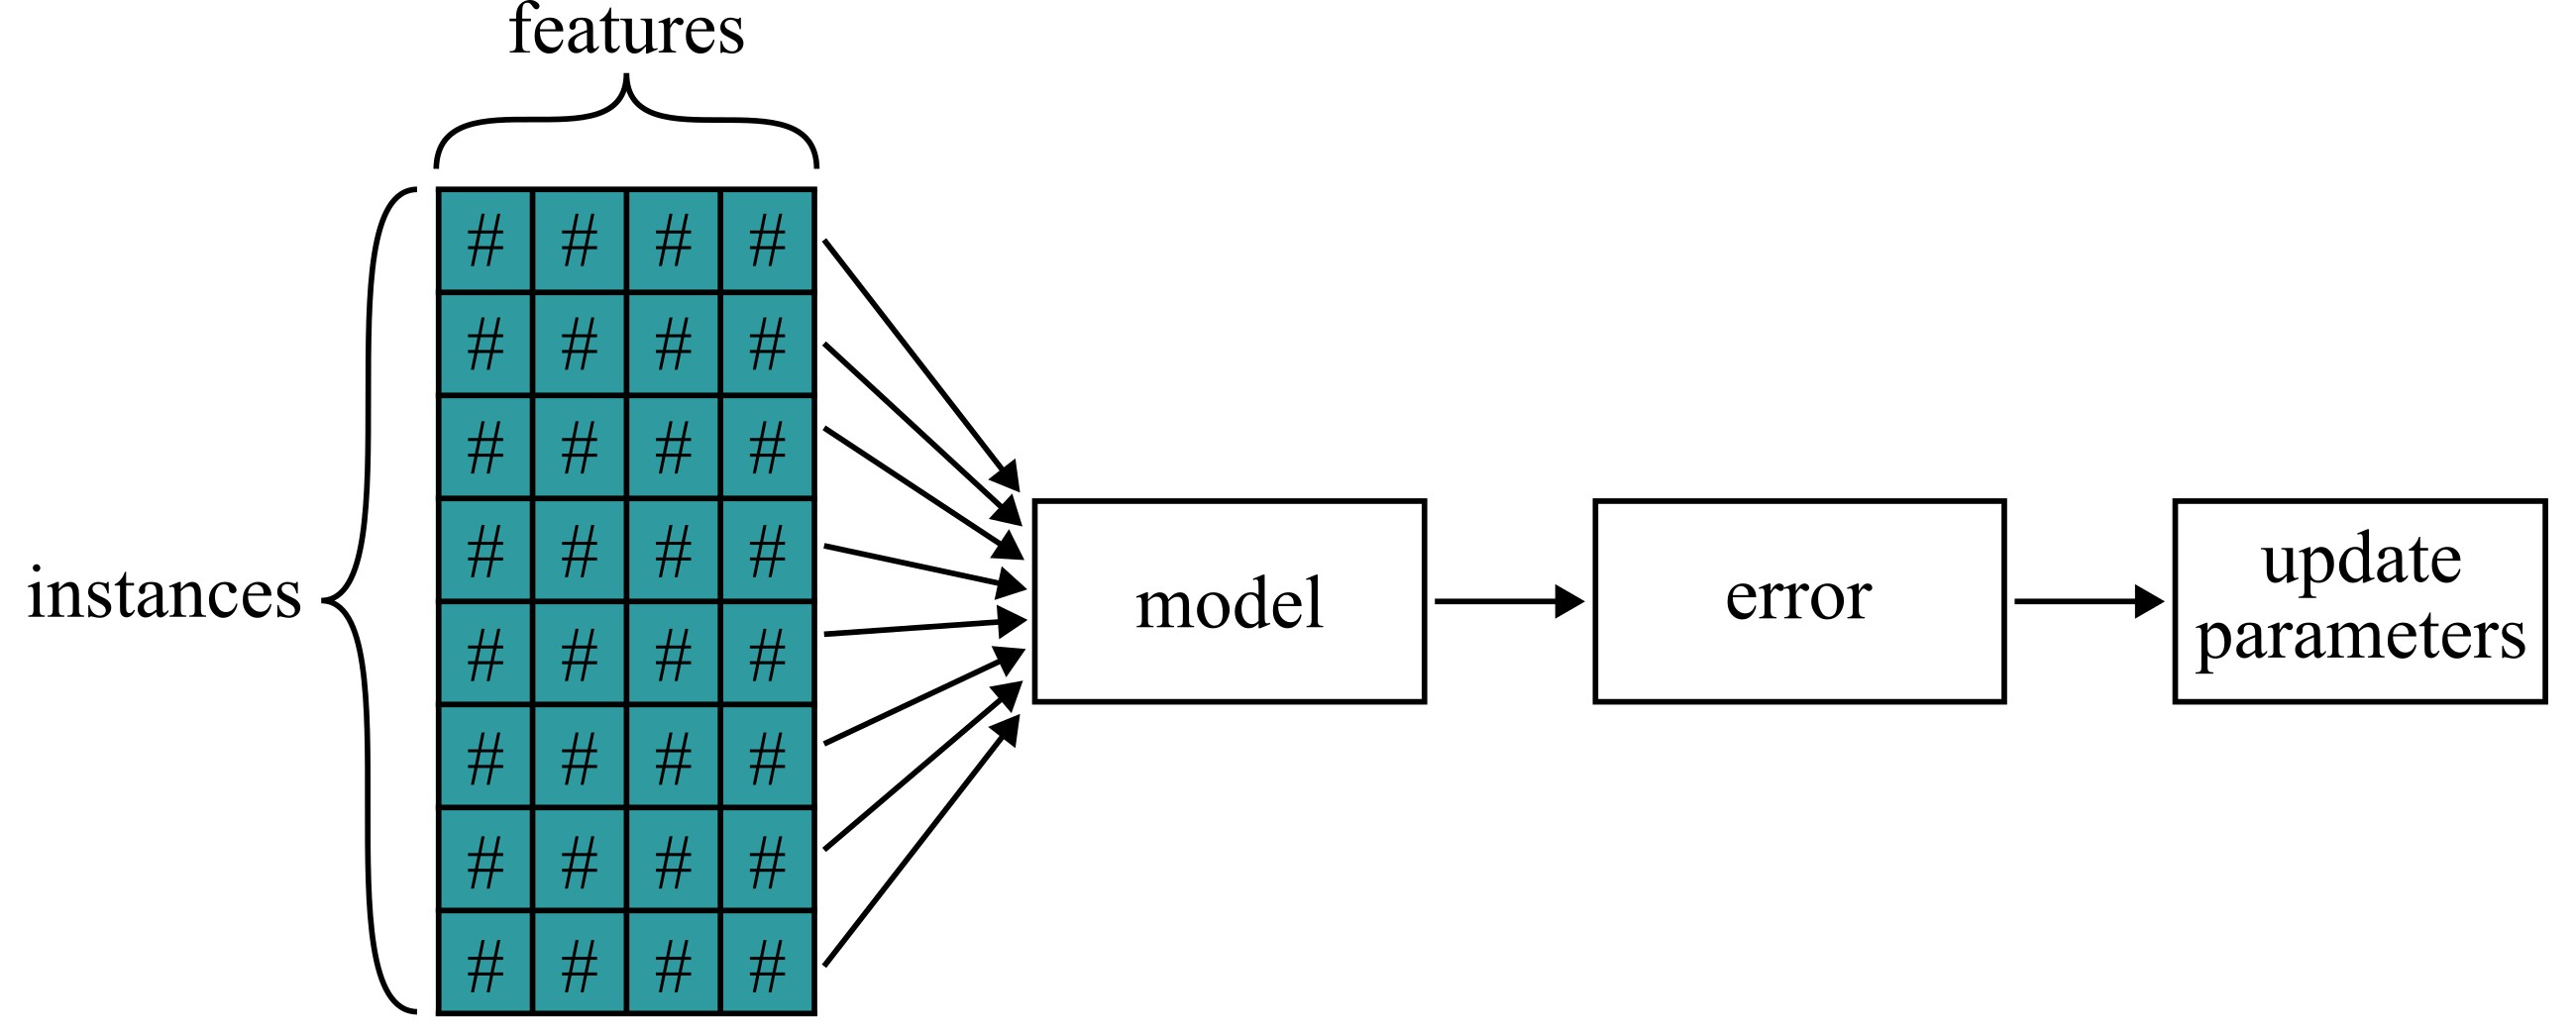
\includegraphics[width=5.3in]{../figures/gradient_descent_batch}
	\caption{Flowchart of Batch Gradient Descent.}
	\label{fig:gradient_descent_batch}
\end{figure}


With this foundation, we can implement gradient descent by computing the gradient of the cost function with respect to each parameter $\theta_j$. Specifically, this involves calculating how much the cost function changes when $\theta_j$ is altered slightly. This calculation is known as a partial derivative. Conceptually, it is akin to determining ``the slope of the mountain under my feet if I face east,'' then repeating the question facing north, and similarly for any other direction in a higher-dimensional space. The partial derivative of the cost function with respect to parameter $\theta_j$ is computed as:
\begin{equation}
\frac{\partial}{\partial \theta_j} J(\theta) = \frac{2}{m} \sum_{i=1}^{m}(\pmb{\theta}^\text{T}\textbf{x}^{(i)} - y^{(i)}) x_j^{(i)}
\label{eq:pd_cost_function}
\end{equation}




Rather than computing each partial derivative individually, all partial derivatives can be calculated simultaneously using the gradient vector, $\nabla_\theta J(\pmb{\theta})$, which encompasses all partial derivatives of the cost function for each model parameter:
\begin{equation}
	\nabla_\theta J(\pmb{\theta}) = \begin{pmatrix}
	\frac{\partial}{\partial \theta_0} J(\theta) \\
	\frac{\partial}{\partial \theta_1} J(\theta) \\
	\vdots  \\
	\frac{\partial}{\partial \theta_n} J(\theta)
	\end{pmatrix}
	= \frac{2}{m} \textbf{X}^\text{T} \cdot (\textbf{X} \pmb{\theta} - \textbf{y})
\end{equation}

\begin{mdframed}[middlelinewidth=0.5mm]
\begin{center}
\rd{WARNING}
\end{center}
Be aware that this method computes using the entire training set $\textbf{X}$ at every step of Gradient Descent, which is why the approach is named Batch Gradient Descent. Although this method can be exceedingly slow with large training sets, it performs well with numerous features, outpacing the Normal Equation in training Linear Regression models with extensive features.
\end{mdframed}

\pagebreak

Once you obtain the gradient vector, which indicates the direction of ascent, the next step involves moving in the opposite direction, effectively going downhill. This is achieved by subtracting $\nabla_\theta J(\theta)$ from $\pmb{\theta}$, incorporating the learning rate $\eta$ to scale the step size:
\begin{equation}
\pmb{\theta}^{(\text{next step})} = \pmb{\theta} - \eta \nabla_\theta J(\pmb{\theta})
\end{equation}

Interestingly, this process aligns perfectly with the results from the Normal Equation. However, variations in the learning rate $\eta$ can significantly influence the outcomes. Figure~\ref{fig:learning_rates} illustrates the first 10 steps of Gradient Descent with three different learning rates, with the dashed line marking the starting point.




		\begin{figure}[H]
			\centering
			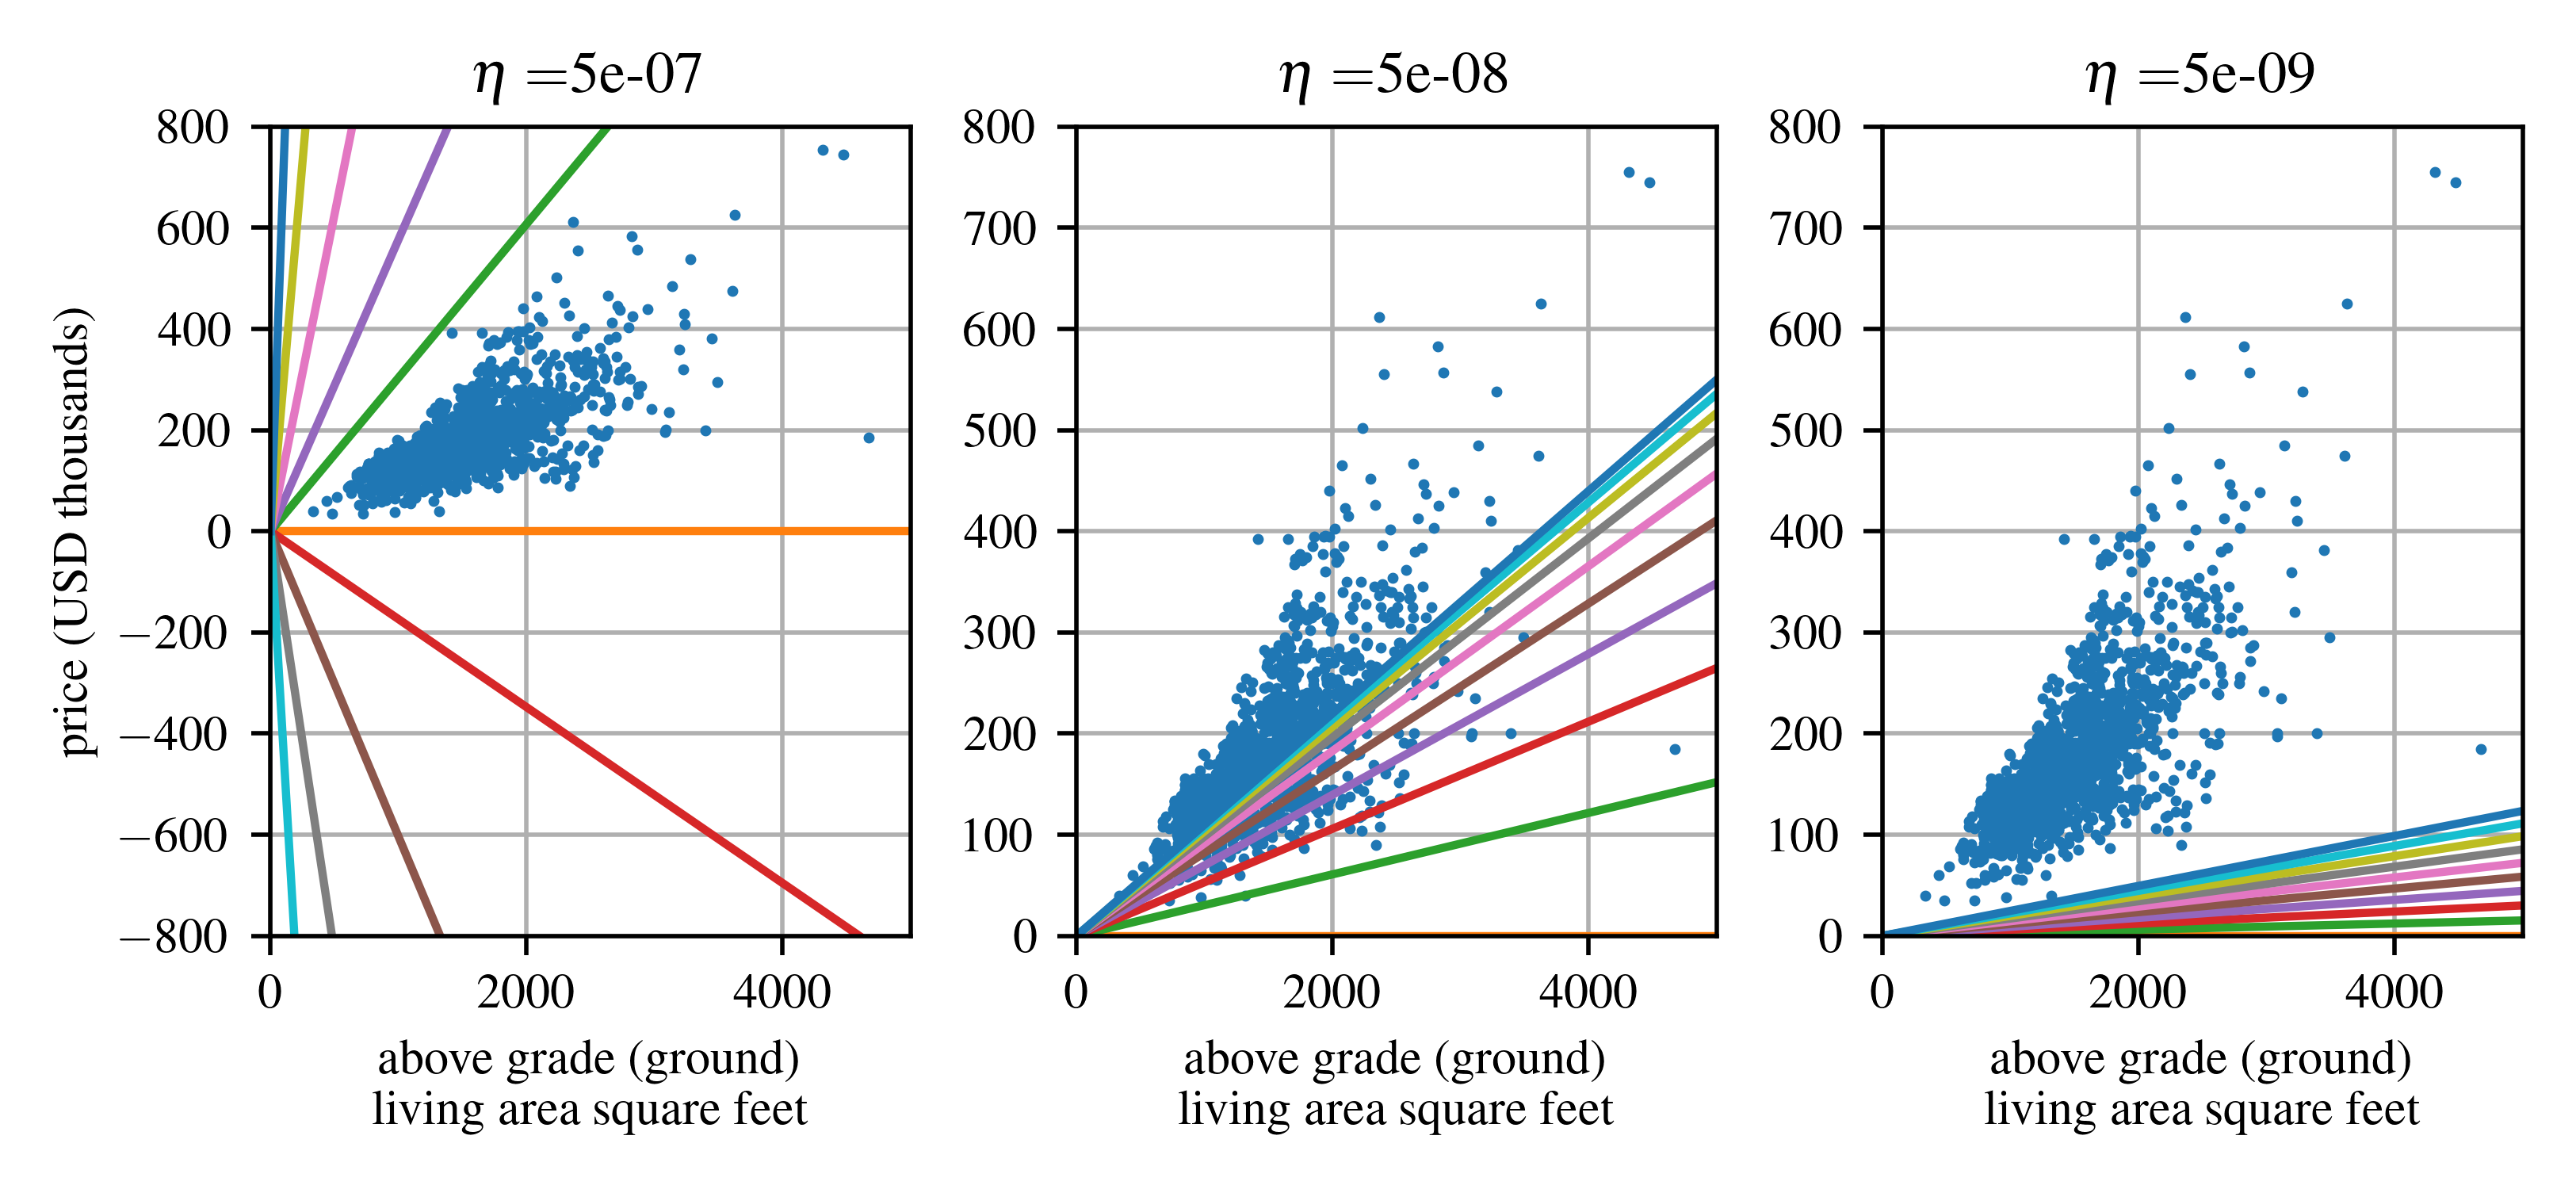
\includegraphics[width=6.5in]{../figures/Ames_learning_rates.png}
			\caption{The effects of different learning rates on the gradient descent algorithms, showing: (a)~too high ($\eta = 5e-07$); (b)~about right ($\eta = 5e-08$), and; (c)~too low ($\eta = 5e-09$).}
			\label{fig:learning_rates}
		\end{figure}


Figure~\ref{fig:learning_rates} highlights the impact of the learning rate on gradient descent.  
Figure~\ref{fig:learning_rates}(a) With a very large step size, \(\eta = 5\times10^{-7}\), each update overshoots the minimum so the algorithm diverges rather than converging.  
Figure~\ref{fig:learning_rates}(b) Using \(\eta = 5\times10^{-8}\) provides a balanced step size; the cost decreases just right~\protect\footnotemark[1] and the algorithm reaches the optimum in only a few iterations.  \footnotetext[1]{Pyle, K. ``Goldilocks and the three bears.'' Mother's Nursery Tales (1918): 207-213.} 
Figure~\ref{fig:learning_rates}(c) A small step size, \(\eta = 5\times10^{-9}\), keeps the algorithm moving toward the minimum yet progress is slow, requiring many more iterations to achieve the same result.


	




To identify an appropriate learning rate, a grid search can be employed. It is advisable to limit the number of iterations during grid search to avoid models that are too slow to converge.

Determining the correct number of iterations is also crucial. If set too low, the algorithm may stop far from the optimal solution. Conversely, overly high settings lead to unnecessary computations after convergence. A practical approach is to allow a large number of iterations but to halt the algorithm when the gradient vector's norm shrinks to below a small threshold $\epsilon$ (known as the tolerance), indicating proximity to the minimum.


\begin{figure}[h]
	\centering
	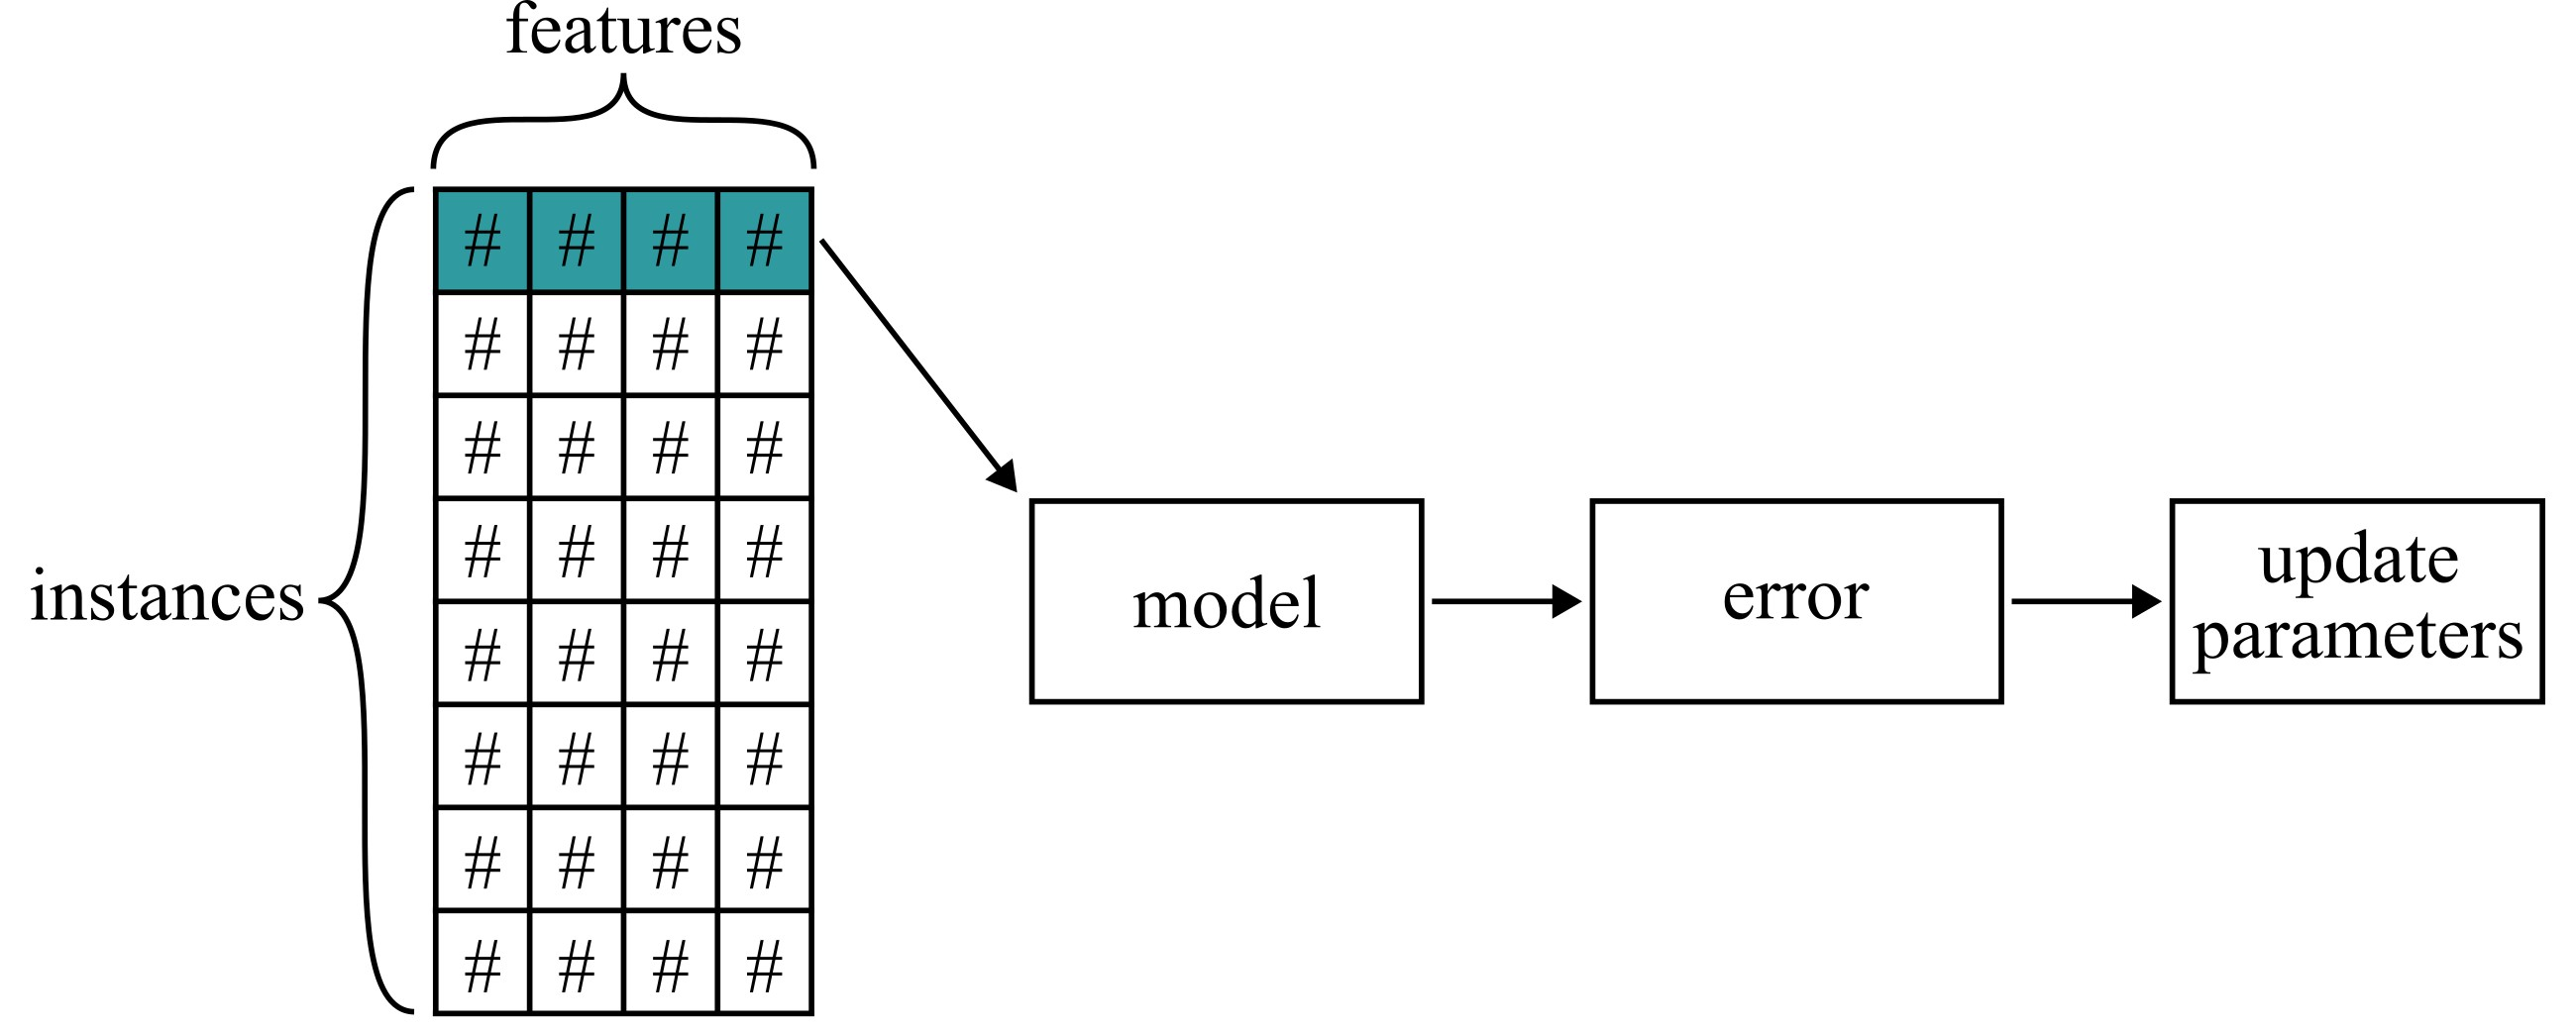
\includegraphics[width=5.4in]{../figures/gradient_descent_stochastic}
	\caption{Flowchart of Stochastic Gradient Descent.}
	\label{fig:gradient_descent_stochastic}
\end{figure}


\subsubsection{Stochastic Gradient Descent}



Stochastic Gradient Descent (shown in figure~\ref{fig:gradient_descent_stochastic}) updates the model parameters after evaluating each individual training sample $x^{(i)}$ and its corresponding label $y^{(i)}$, which stands in contrast to batch gradient descent that uses the entire dataset for each update. The update rule for SGD can be expressed as



\begin{equation}
\theta^{(\text{next step})} = \theta - \eta \nabla_\theta J(\theta; x^{(i)}; y^{(i)}).
\end{equation}

While batch gradient descent tends to perform unnecessary recalculations for large datasets by reevaluating gradients for similar examples with each update, SGD eliminates this inefficiency by updating parameters incrementally. Consequently, SGD is generally faster and adaptable for online learning.
Due to its frequent and individual updates, SGD exhibits high variance in the objective function, causing significant fluctuations as illustrated in Fig.~\ref{fig:stochastic_gradient_descent_target}(b).


\begin{figure}[H]
	\centering
	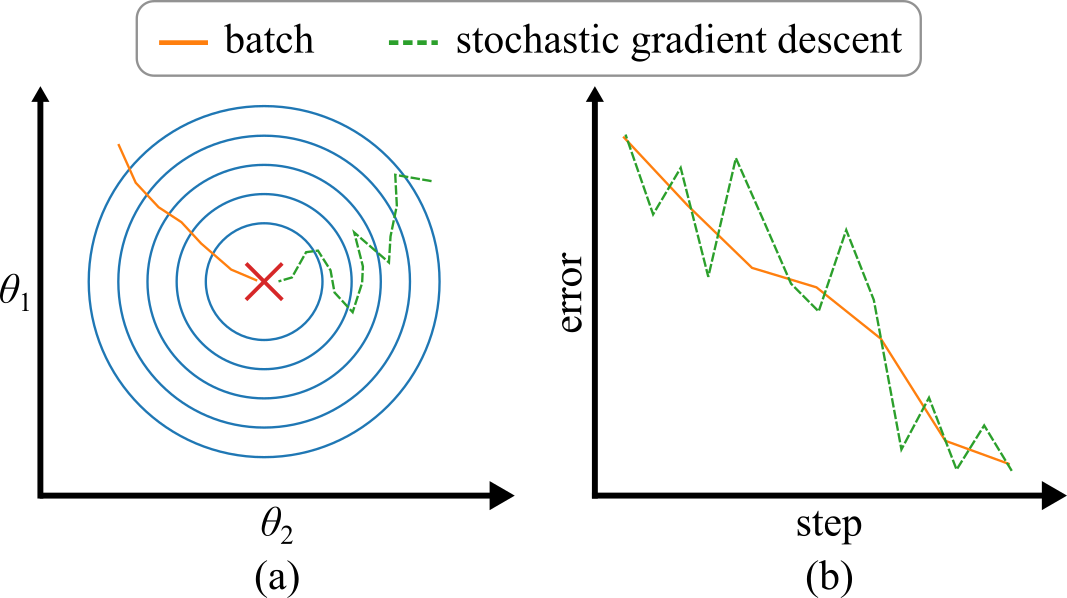
\includegraphics[]{../figures/stochastic_gradient_descent_target}
	\caption{Comparison of the iterative performance of Batch and Stochastic Gradient Descent, showing: (a) how they move towards their target, and (b) the error at comparable steps.}
	\label{fig:stochastic_gradient_descent_target}
\end{figure}



\pagebreak


\subsubsection{Mini-batch Gradient Descent}


\begin{figure}[H]
	\centering
	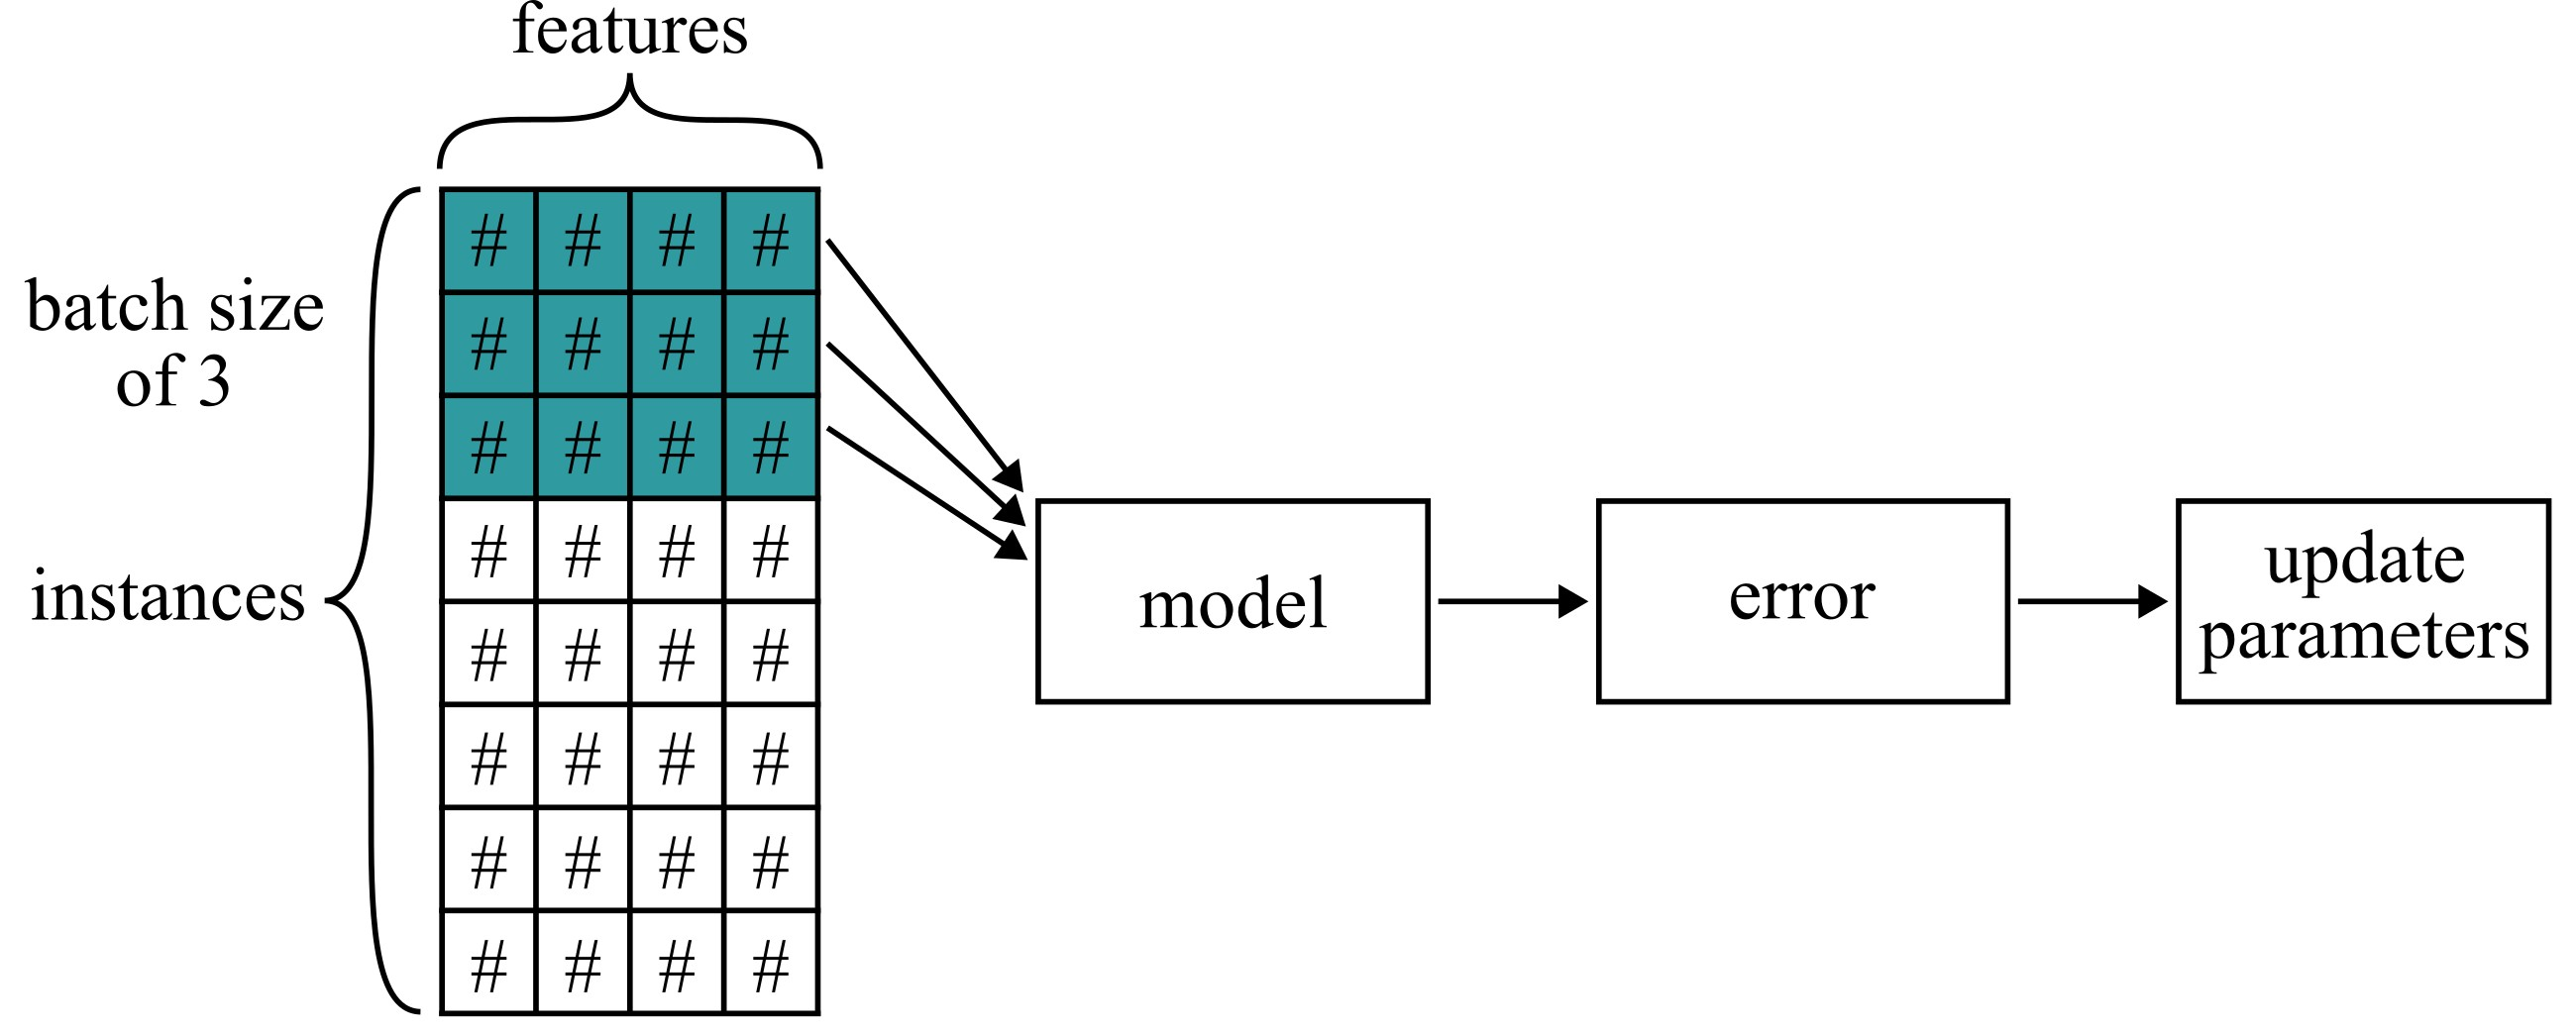
\includegraphics[width=5.4in]{../figures/gradient_descent_mini_batch}
	\caption{Flowchart of Mini-batch Gradient Descent.}
	\label{fig:gradient_descent_mini_batch}
\end{figure}


\begin{equation}
\theta^{(\text{next step})} = \theta - \eta \nabla_\theta J(\theta; x^{(i:i+n)}; y^{(i:i+n)})
\end{equation}

The final Gradient Descent algorithm we will discuss is Mini-batch Gradient Descent. This method combines elements of both Batch and Stochastic Gradient Descent: rather than calculating gradients using the entire training set (as in Batch GD) or a single instance (as in Stochastic GD), Mini-batch GD computes gradients using small, randomly selected subsets of instances known as minibatches. One significant benefit of Mini-batch GD over Stochastic GD is the improved performance from hardware-optimized matrix operations, particularly on GPUs.

Mini-batch GD's trajectory through parameter space tends to be more stable compared to the often erratic path of SGD, especially with larger minibatches. This stability typically brings Mini-batch GD closer to the minimum than SGD. However, Mini-batch GD might struggle more with escaping local minima in scenarios prone to such issues, which is less of a concern in Linear Regression. Figure~\ref{fig:Comparing_gradient_descent_methods} illustrates the trajectories of these three Gradient Descent techniques during training. While Batch GD precisely reaches the minimum, Stochastic GD and Mini-batch GD tend to oscillate nearby. It is important to note, however, that while Batch GD is slow in taking steps, both Stochastic GD and Mini-batch GD could also effectively reach the minimum with an appropriate learning rate schedule.




\subsubsection{Feature Scaling}

The cost function can resemble an elongated bowl if the feature scales vary significantly. Figure~\ref{fig:gradient_descent_5} illustrates the effect of feature scaling on Gradient Descent. In figure~\ref{fig:gradient_descent_5}(a), Gradient Descent progresses directly towards the minimum, reaching it swiftly. However, in figure~\ref{fig:gradient_descent_5}(b) it initially moves almost orthogonally to the direction of the global minimum, followed by a lengthy traverse down a nearly flat valley, significantly delaying the convergence.

\begin{figure}[H]
    \centering
    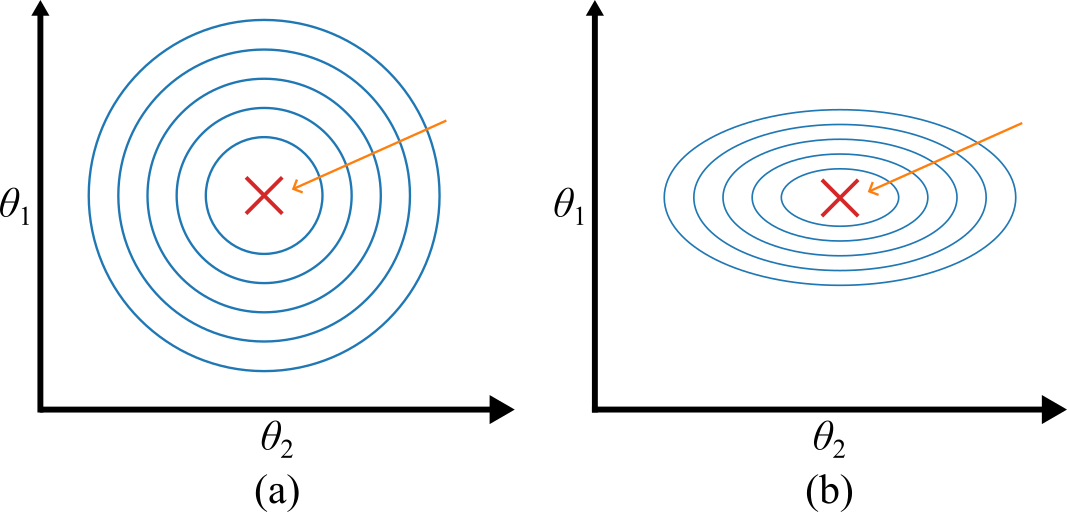
\includegraphics[]{../figures/gradient_descent_5.png }
		\vspace{-1ex}
    \caption{Gradient descent on a 2D surface for parameters that are: (a) equally scaled, and (b) unequally scaled.}
		\vspace{-1ex}
    \label{fig:gradient_descent_5}
\end{figure}



Training a model can be viewed as a search through the parameter space for the combination that minimizes the cost function. When additional parameters are introduced, this space gains extra dimensions, making the optimization task more challenging. In Ordinary Least Squares Linear Regression, however, the cost surface is convex and bowl-shaped, so any descent method is guaranteed to reach the global minimum. To normalize feature scales, two common methods are employed. The are Min-max scaling and Standardization. 
\begin{itemize}
\item \textbf{Min-max scaling}, often referred to as normalization, is straightforward: it rescales the data to a range of 0 to 1 by subtracting the minimum value and dividing by the range (max minus min).
\begin{equation}
\textbf{X}' = \frac{\textbf{X} - \textbf{X}_\text{min}}{\textbf{X}_\text{max} - \textbf{X}_\text{min}}
\end{equation}
Scikit-Learn offers \texttt{sklearn.preprocessing.MinMaxScaler} for this purpose.
\item \textbf{Standardization} differs significantly as it first subtracts the mean (resulting in a zero mean) and then divides by the standard deviation to achieve unit variance. This method does not limit values to a specific range, which can be problematic for certain algorithms, such as neural networks which often expect inputs between 0 and 1. However, standardization is less sensitive to outliers. For instance, if a median income is mistakenly recorded as 100, min-max scaling would compress all other values between 0 and 15 to between 0 and 0.15, whereas standardization would be minimally affected.
\begin{equation}
\textbf{X}' = \frac{\textbf{X} - \overline{\textbf{X}}}{\sigma}
\end{equation}
\texttt{sklearn.preprocessing.StandardScaler} is provided by Scikit-Learn for standardization.
\end{itemize}

\begin{mdframed}[middlelinewidth=0.5mm]
\begin{center}
\rd{WARNING}
\end{center}
It is crucial to apply scalers exclusively to the training data and not to the entire dataset, which includes the test set. This practice ensures that the model is not inadvertently exposed to test data during training. Once the scalers are fitted to the training data, they can then be used to transform the training set, the test set, and any new data subsequently encountered.
\end{mdframed}


\pagebreak





\subsection{Polynomial Regression }



%\todo{Need to dicuss Bias and , include\_bias=False in sk.preprocessing.PolynomialFeatures. Why does this not need a bias? More math would be helpful. }


What if the underlying pattern of your data is more complex than a simple linear relationship? Consider the dataset shown in figure~\ref{fig:Polynomial_1} with non-linear characteristics (one feature across multiple instances), which typically can be modeled using a second-order polynomial
\begin{equation}
\hat{y}=ax^2+bx+c.
\label{eq:poly}
\end{equation}


\begin{figure}[H]
	\centering
	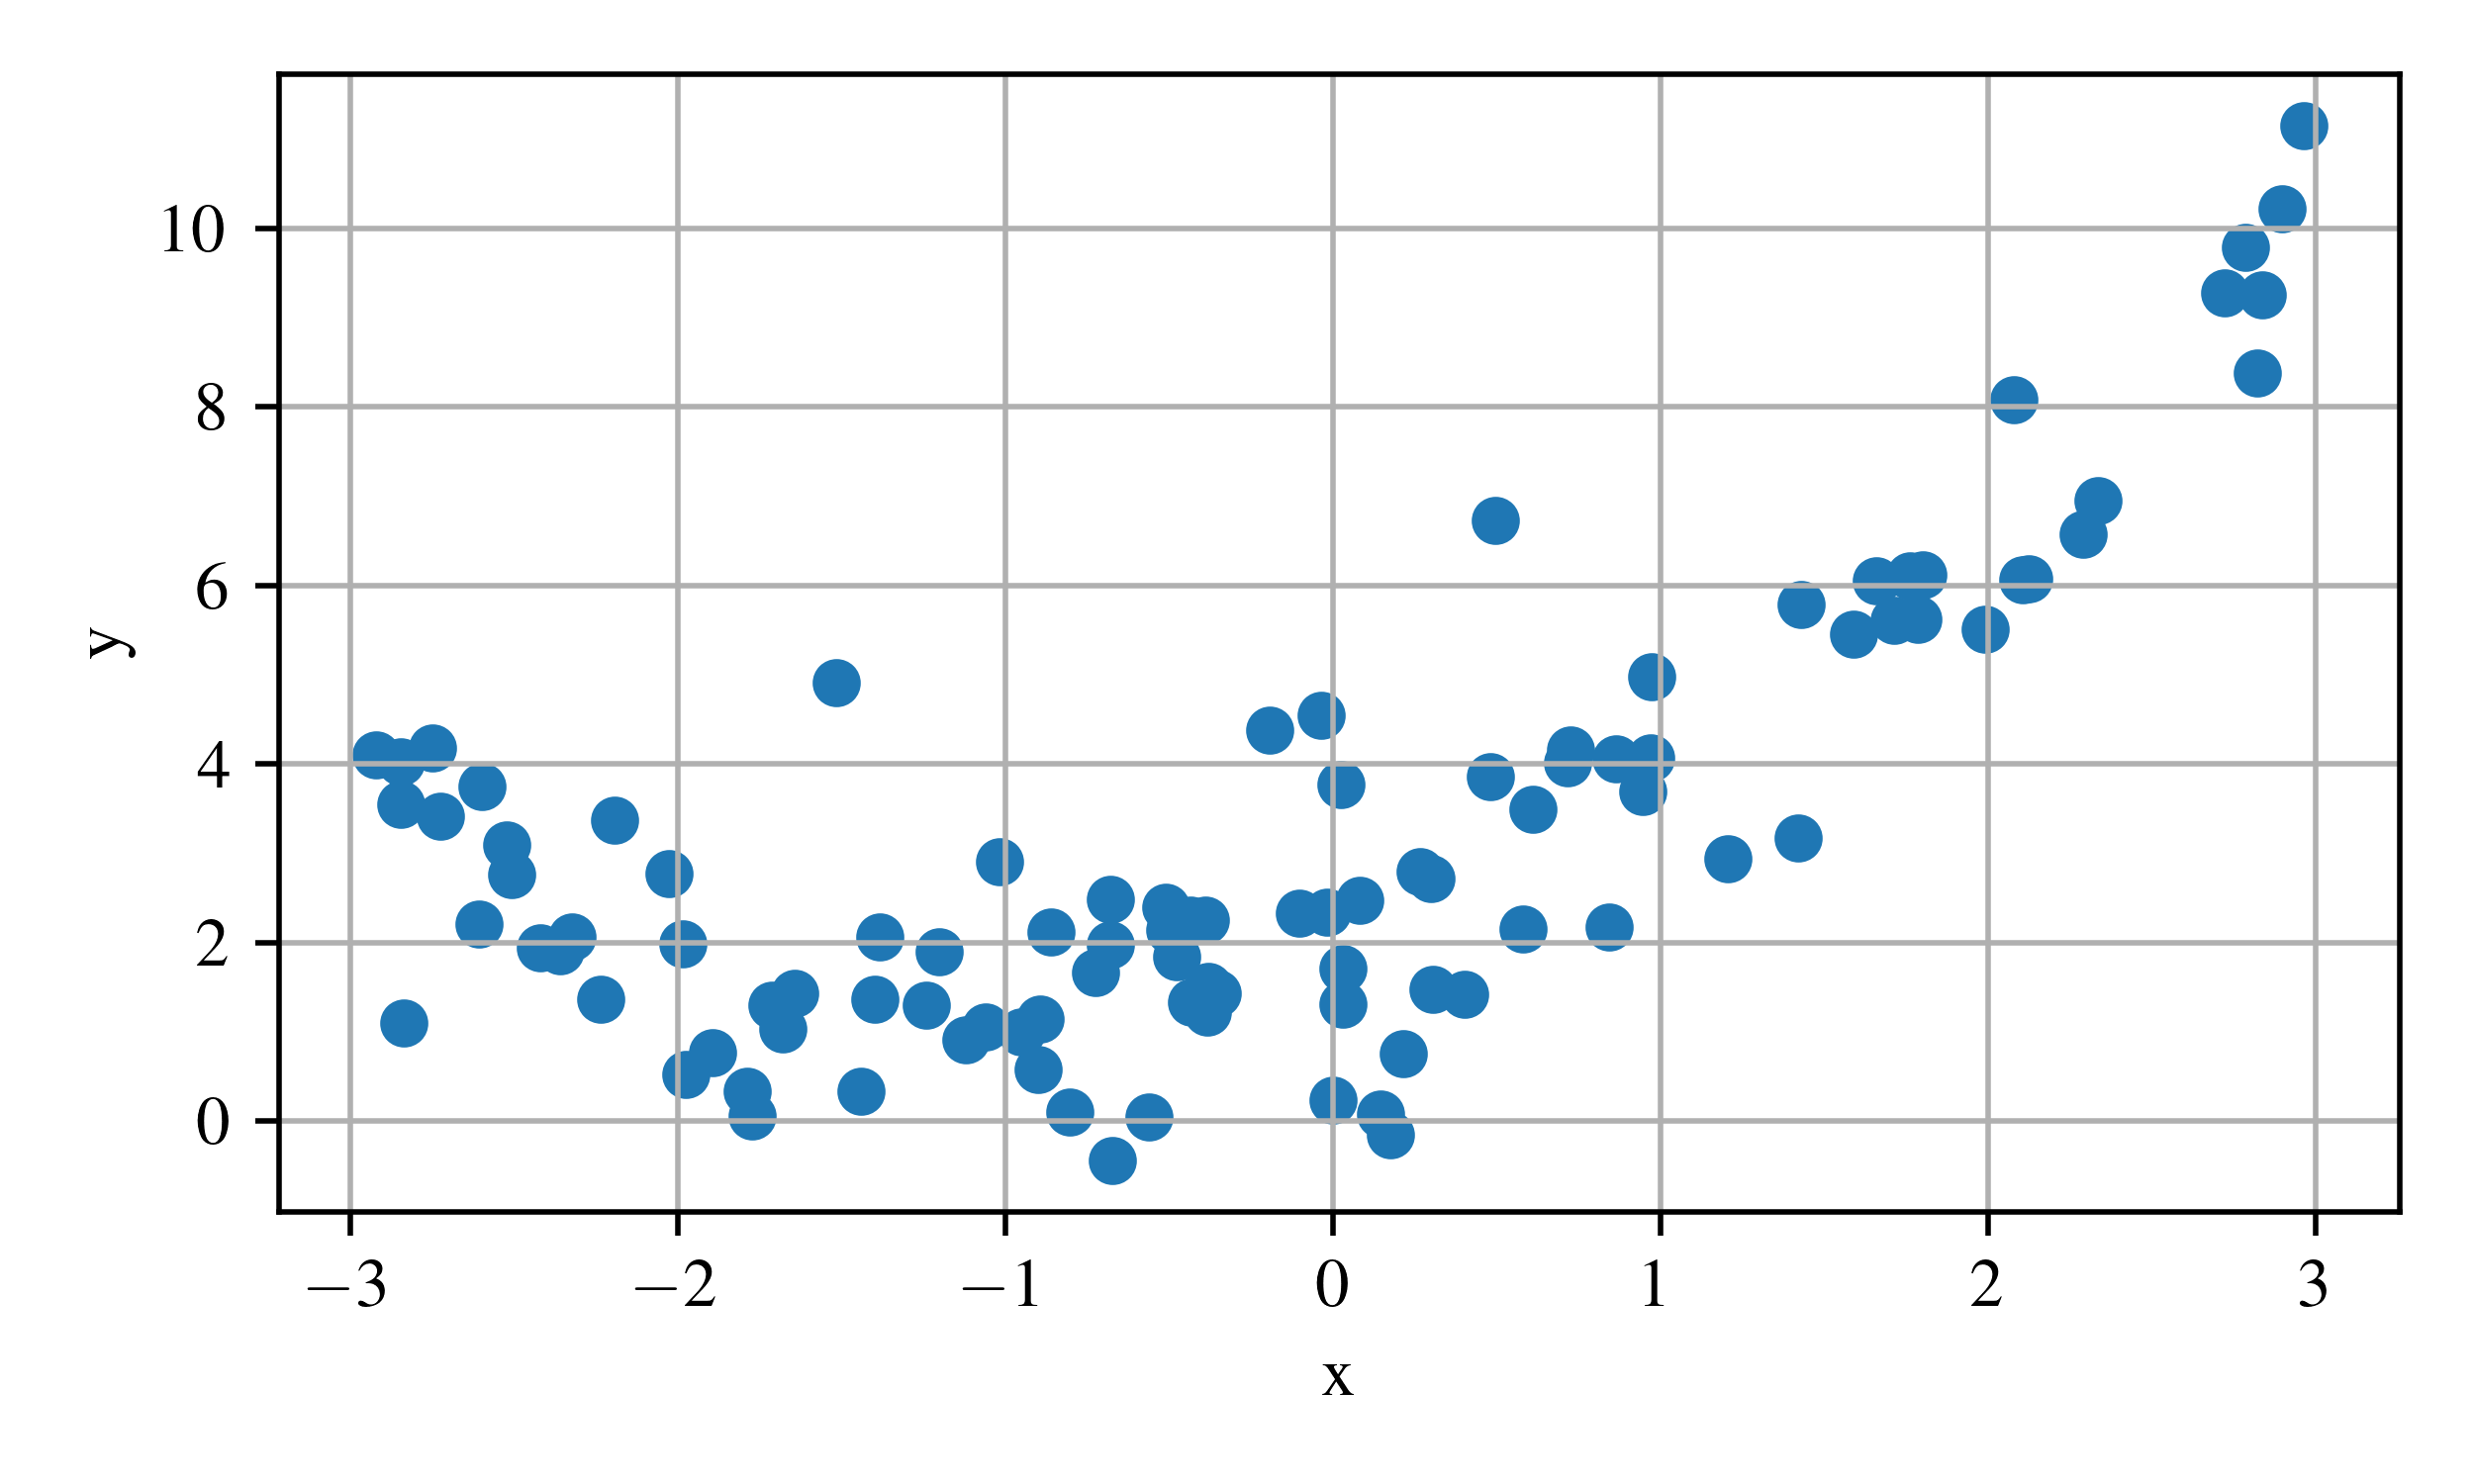
\includegraphics[width=4in]{../figures/polynomial_regression_1}
	\caption{Dataset derived from a 2\textsuperscript{nd}-order polynomial.}
	\label{fig:Polynomial_1}
\end{figure}

%\todo{need to talk about how this is only one feature, and we build off of that. }
%\url{https://medium.com/analytics-vidhya/understanding-polynomial-regression-5ac25b970e18}

A simple linear fit will under-perform, so you first enrich the training set by adding the squared term of each feature as an extra column; shown in figure~\ref{fig:Polynomial_2}. Although the model you train is still linear with respect to its parameters, it now operates on an augmented feature space and can represent the desired quadratic curve. This approach is called Polynomial Regression, and it extends naturally by including higher powers whenever more complex nonlinearities are present.


		\begin{figure}[H]
			\centering
			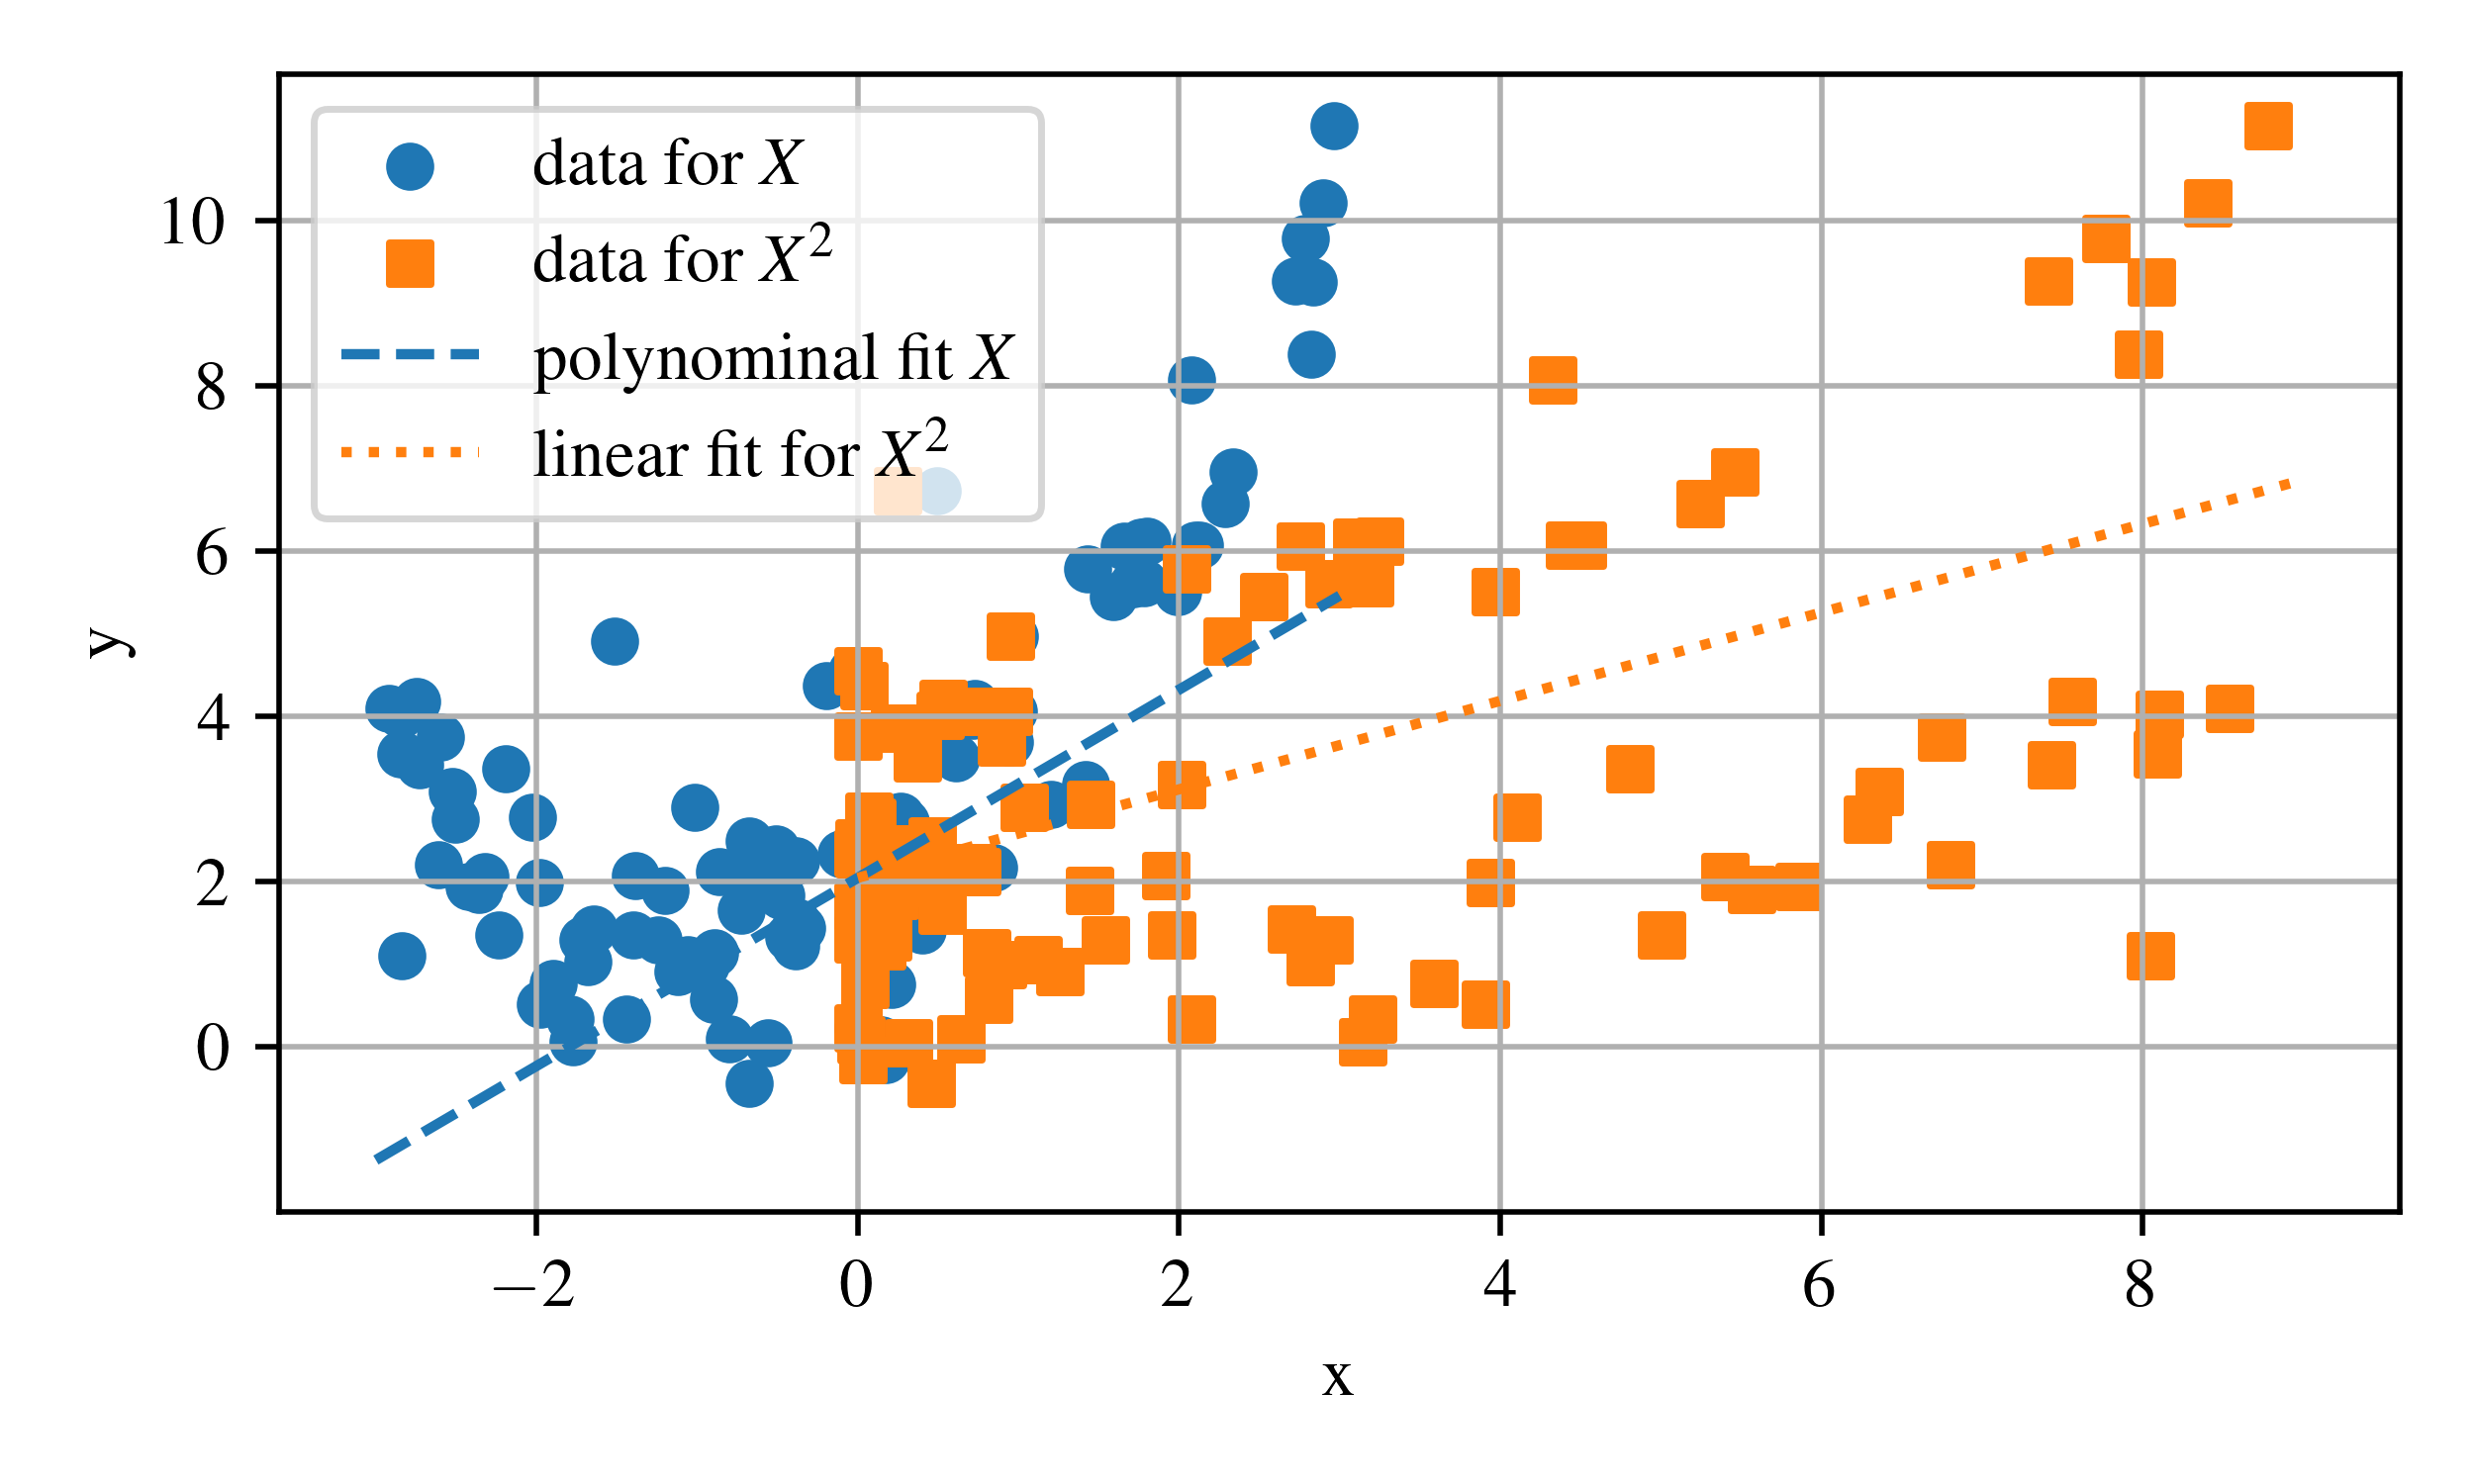
\includegraphics[width=4in]{../figures/polynomial_regression_2}
			\caption{Linear models fit to the individual features of a polynomial dataset.}
			\label{fig:Polynomial_2}
		\end{figure}

\pagebreak
This data can then be incorporated into two linear models, where the slopes of the feature sets serve as the parameters for the base-line polynomial expression ($a$ and $b$ in Equation~\ref{eq:poly}) and the bias term is the offset ($c$ in Equation~\ref{eq:poly}). The results of such a polynomial fit is shown in figure~\ref{fig:Polynomial_3}.


		\begin{figure}[H]
			\centering
			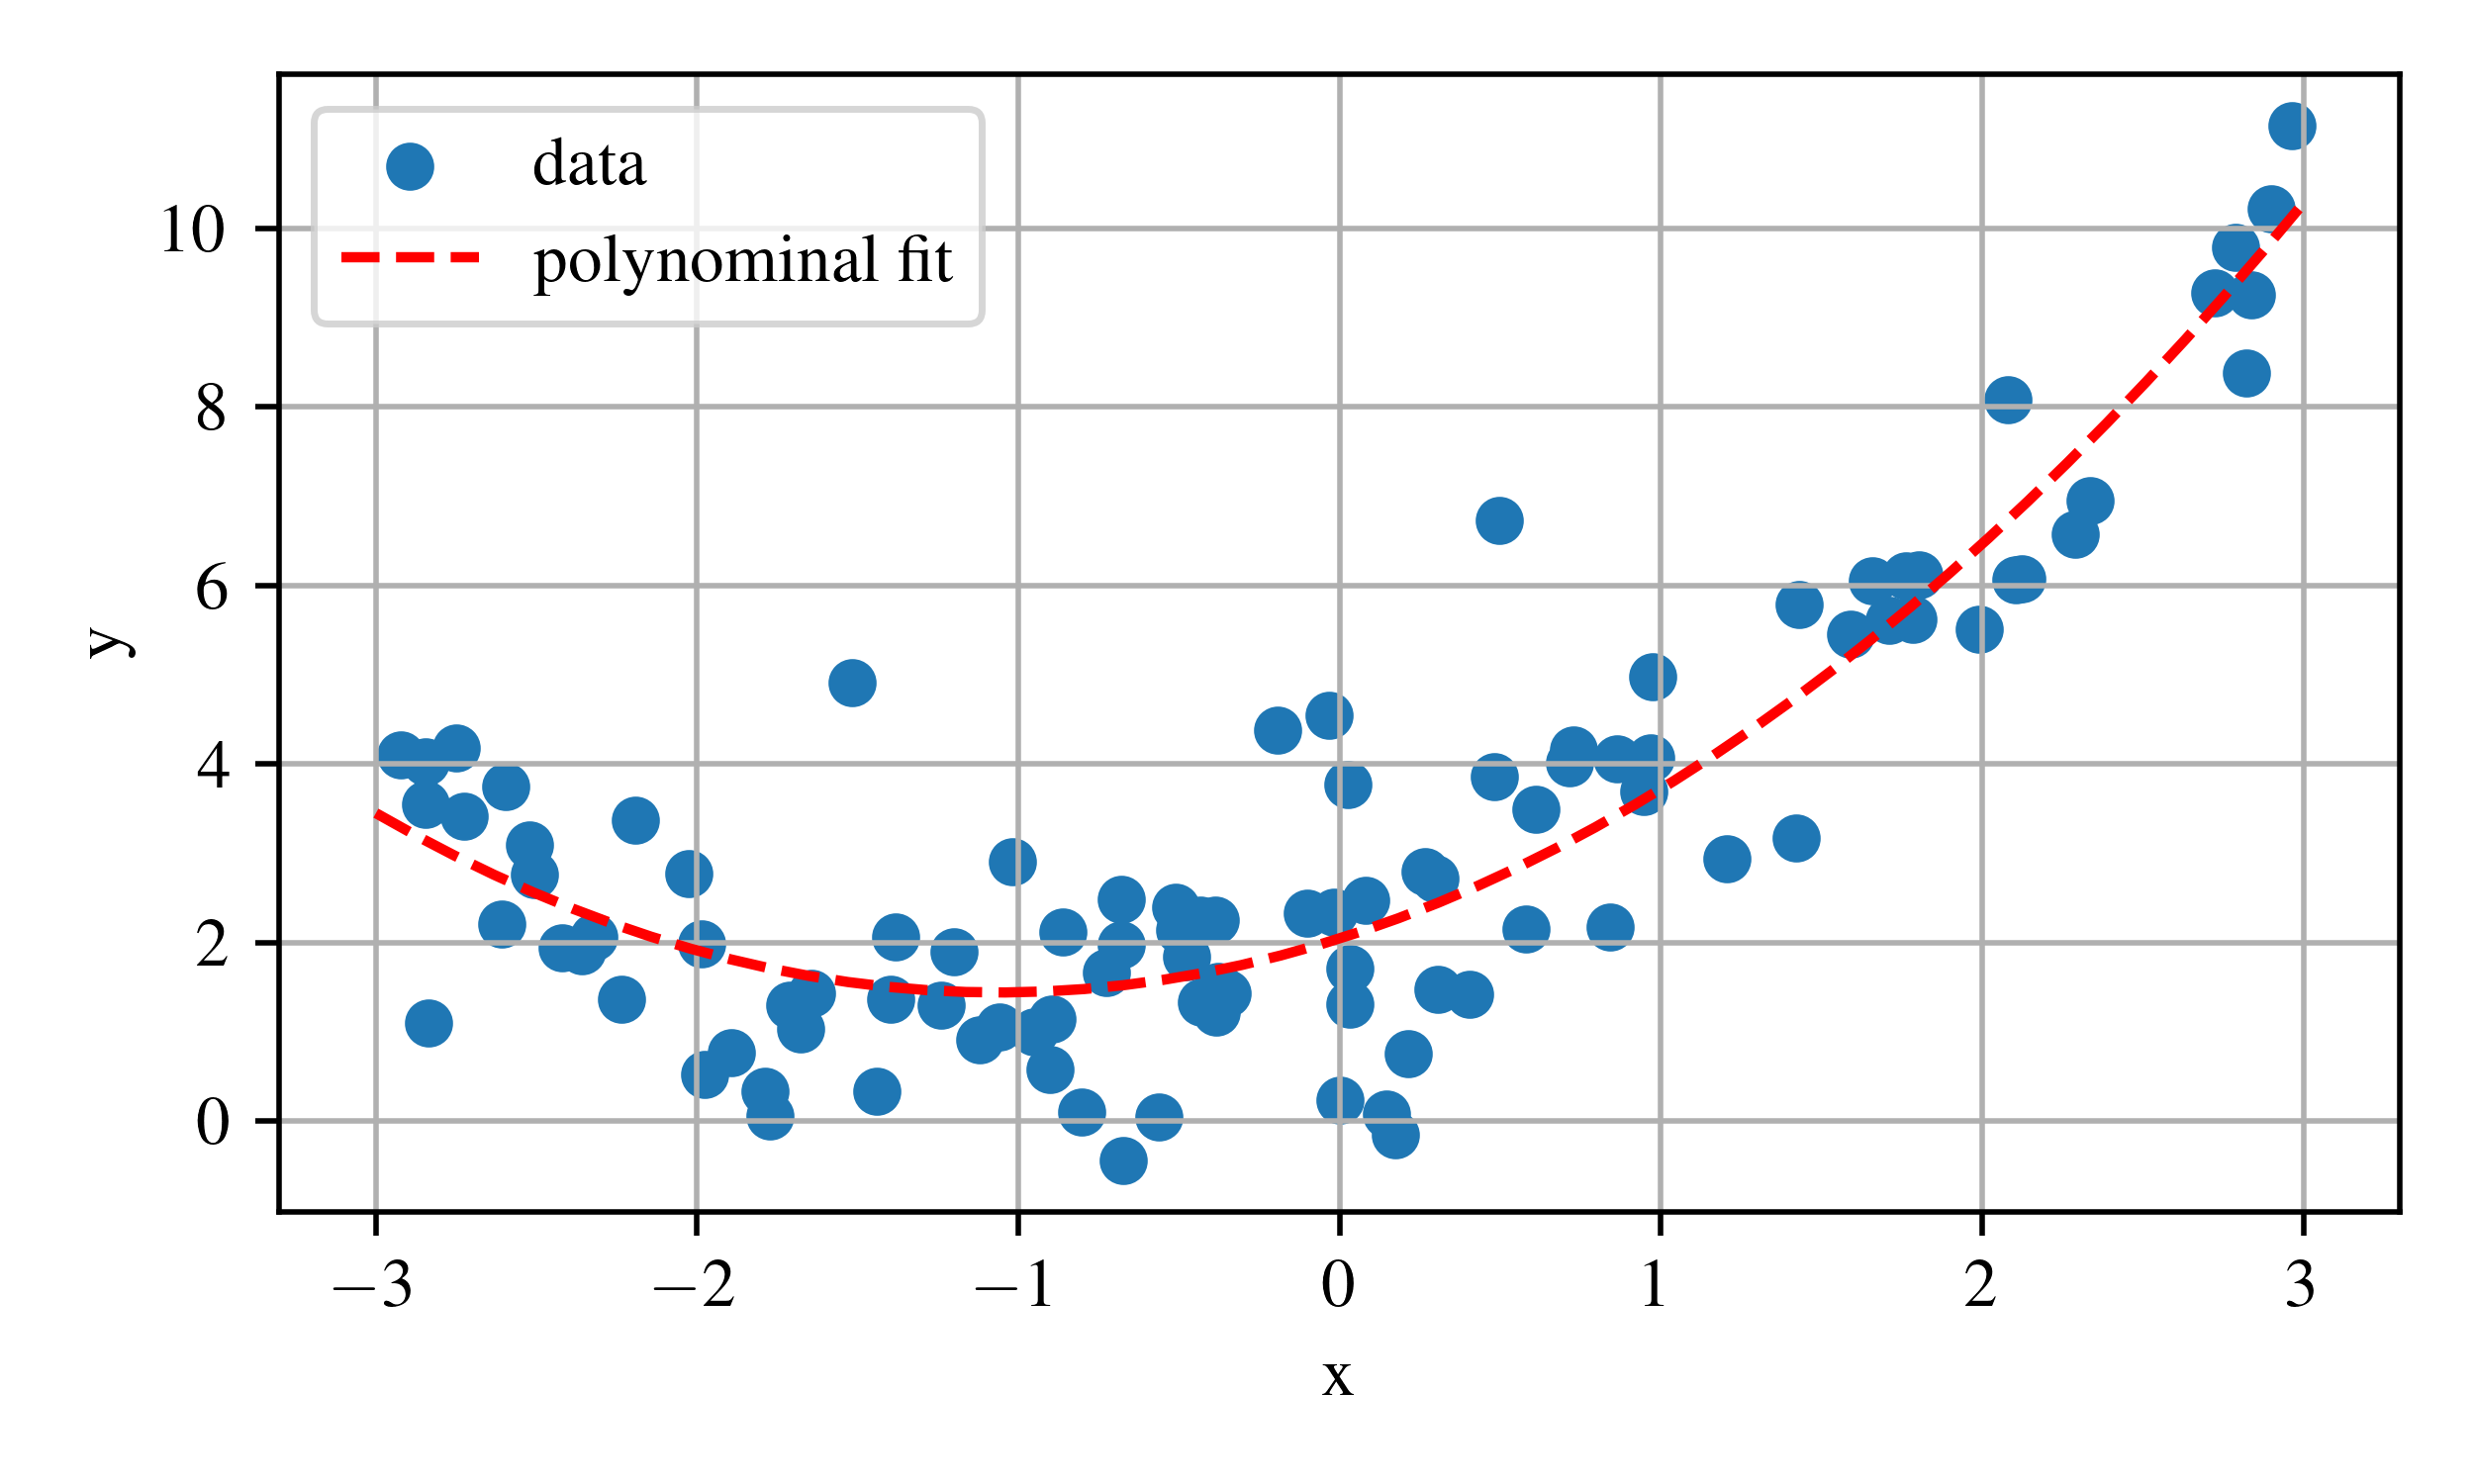
\includegraphics[width=4in]{../figures/polynomial_regression_3}
			\caption{Polynomial model fit to a dataset.}
			\label{fig:Polynomial_3}
		\end{figure}


It is important to note that Polynomial Regression can identify interrelationships between features in cases where multiple features exist, a capability beyond the scope of simple Linear Regression. This enhancement is enabled by \texttt{PolynomialFeatures}, which includes all possible combinations of features up to the specified degree. For instance, with two features $a$ and $b$, and a degree of 3, \texttt{PolynomialFeatures} would add not only $a^2, a^3, b^2,$ and $b^3$ but also the combined terms $ab, a^2b,$ and $ab^2$.



\begin{mdframed}[middlelinewidth=0.5mm]
\begin{center}
\rd{WARNING}
\end{center}
\texttt{PolynomialFeatures(degree=d)} expands an array with $n$ original features into one that includes $\frac{(n+d)!}{d!n!}$ features, accounting for all combinations of features up to the $d$-th degree. Here, $n!$ represents the factorial of $n$, calculated as $1 \times 2 \times 3 \times \cdots \times n$. Be cautious of the rapid increase in the number of features, known as combinatorial explosion!
\end{mdframed}

\begin{example}
\textbf{Polynomial Regression}

\noindent This example fits a non-linear dataset using polynomial regression by adding $x^2$ as an extra feature. It demonstrates how linear models can approximate curved relationships when polynomial terms are included, and shows the resulting fit compared to the original data.
\end{example}


\pagebreak
\subsection{Training and Testing Data}

Training a predictive model on a dataset and then testing it with the same data is a fundamental error in methodology. Such a model could simply memorize the labels of the training samples, achieving perfect performance during training but failing to make any useful predictions on new, unseen data. This phenomenon is known as overfitting. To prevent this, it is standard practice in supervised machine learning to reserve a portion of the available data as a test set, denoted as $\textbf{X}_\text{test}$ and $\textbf{y}_\text{test}$.

		\begin{figure}[H]
			\centering
			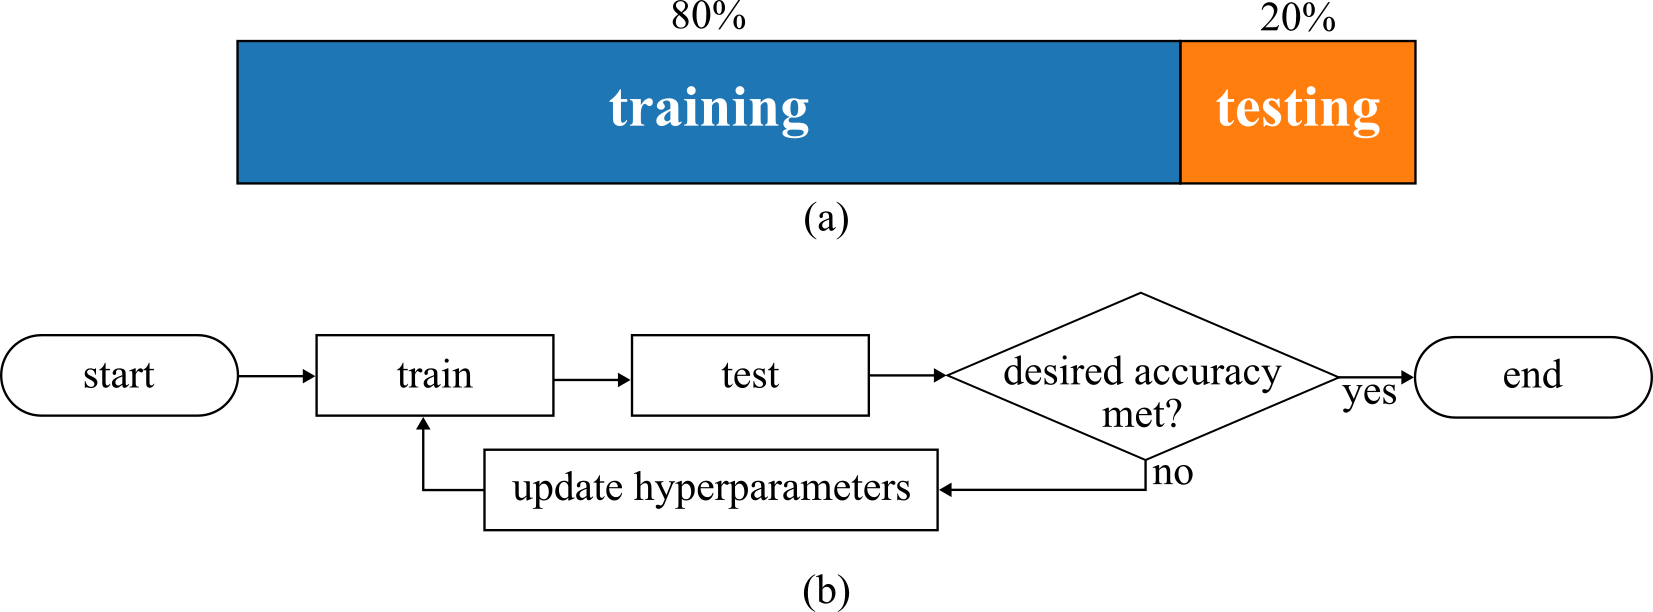
\includegraphics[]{../figures/training_test_datasets}
			\caption{Splitting data up into training and testing subsets.}
			\label{fig:training_test_datasets}
		\end{figure}


		\begin{figure}[H]
			\centering
			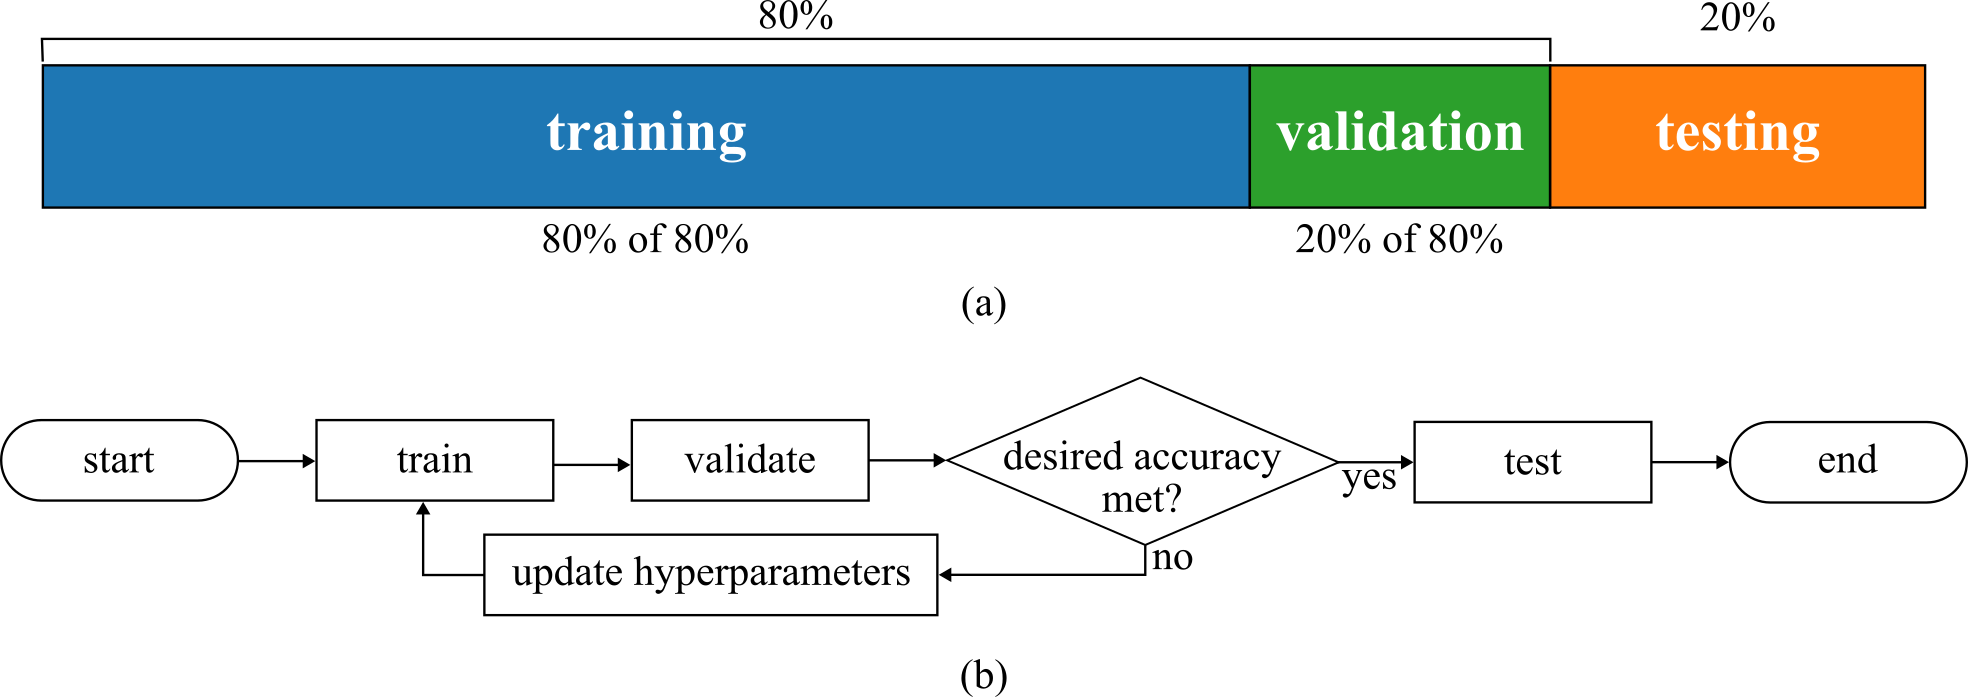
\includegraphics[]{../figures/training_validation_test_datasets}
			\caption{Splitting data up into training, validation, and testing subsets.}
			\label{fig:training_validation_test_datasets}
		\end{figure}


The function \texttt{sklearn.model\_selection.train\_test\_split} in scikit-learn randomly divides arrays or matrices into training and testing subsets.

\pagebreak

\subsection{Pipelines}


Pipelines in scikit-learn streamline the process by sequentially applying a list of transformations followed by a final estimator to a dataset. Employing pipelines allows for the integration of multiple processing steps, which can then be cross-validated together while experimenting with various parameters. Fig.~\ref{fig:AutoML_diagram} illustrates a typical pipeline configuration in scikit-learn.



		\begin{figure}[H]
			\centering
			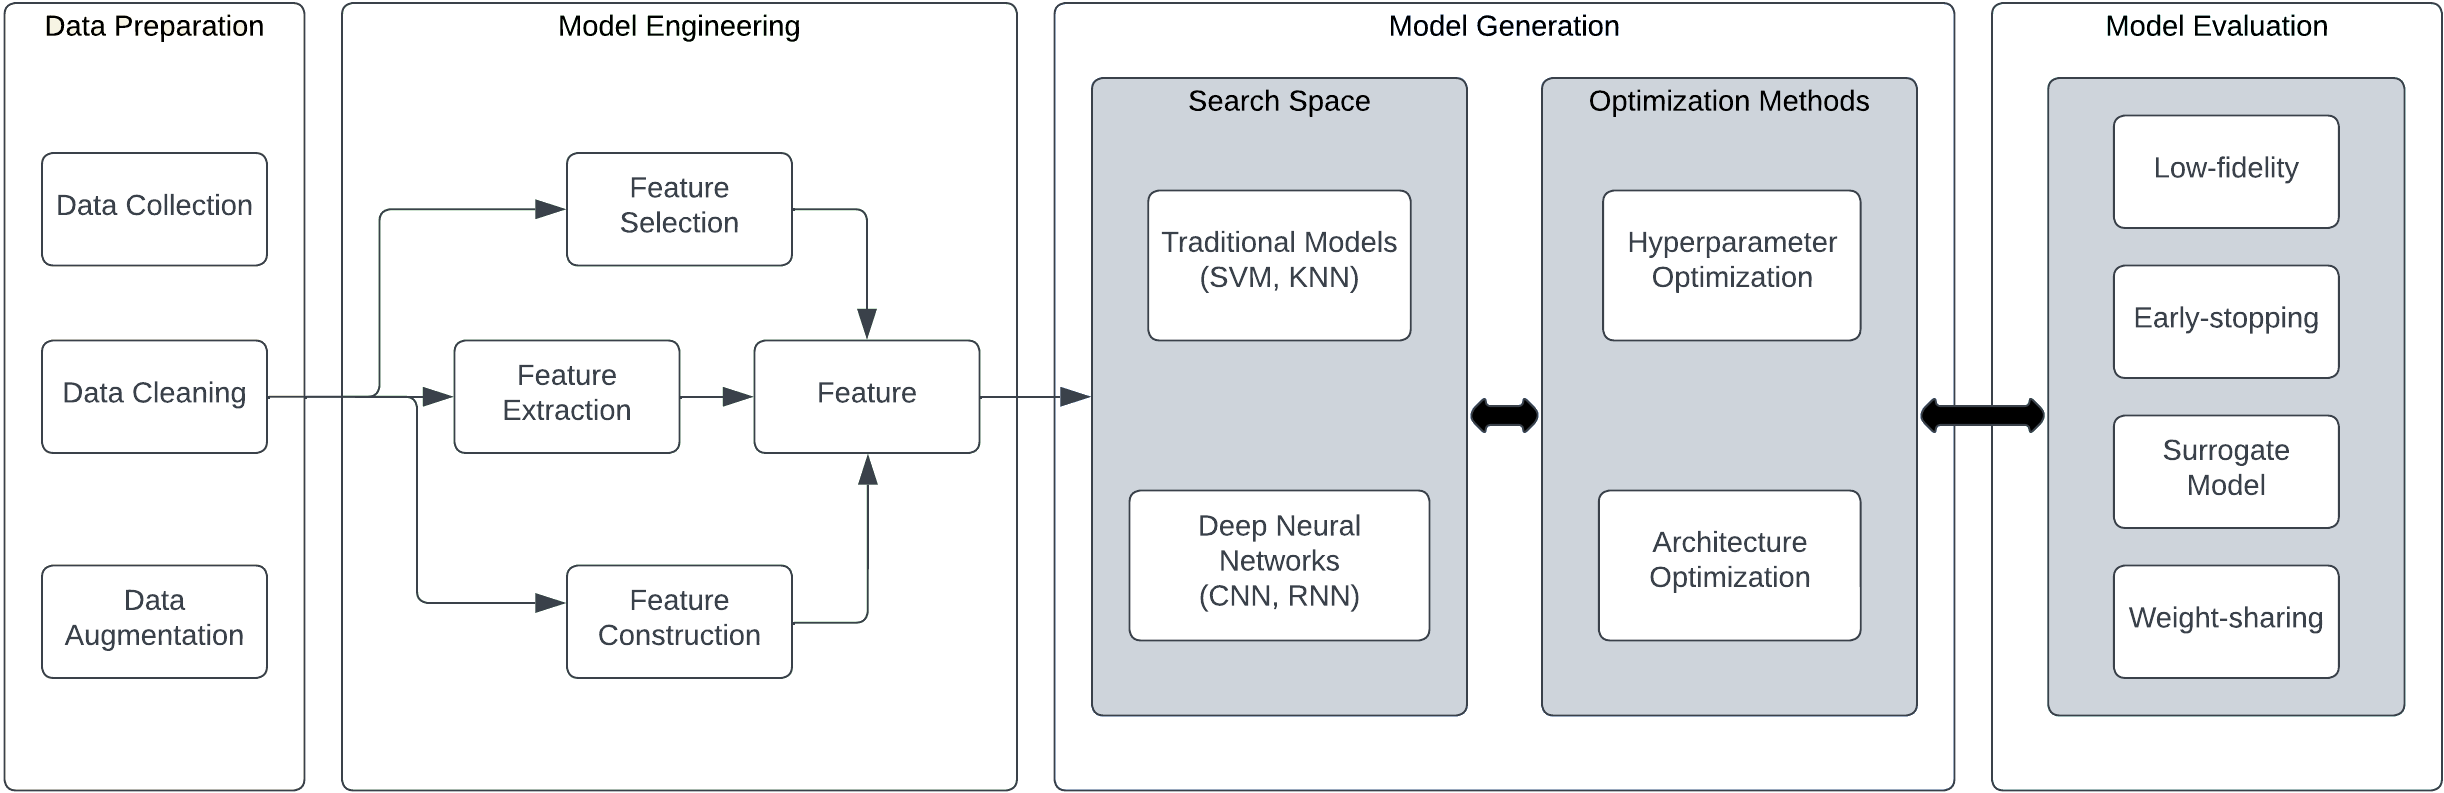
\includegraphics[width=6.5in]{../figures/AutoML_diagram}
			\caption{Pipeline setup for the automated deployment of pre-processing and modeling steps.\protect\footnotemark[1]}
			\label{fig:AutoML_diagram}
		\end{figure}


\footnotetext[1]{Modified from PopovaZhuhadar, CC BY-SA 4.0 $<$https://creativecommons.org/licenses/by-sa/4.0$>$, via Wikimedia Commons}

\subsection{Learning Curves}

Performing Polynomial Regression with a high degree typically allows for a closer fit to the training data compared to simple Linear Regression. For instance, Figure~\ref{fig:overfitting_1} demonstrates the application of a 30-degree polynomial model to a set of training data, contrasting it with both a linear model and a quadratic model (2\textsuperscript{nd}-degree polynomial). Observe how the 30-degree polynomial model contorts to closely match the training instances.
\begin{itemize}
\item The linear model exhibits underfitting.
\item The high-degree Polynomial Regression model drastically overfits the training data.
\item Among these, the quadratic model is likely to generalize best.
\end{itemize}
In this instance, the appropriateness of the quadratic model is clear since the data was initially generated using such a model. However, in real-world scenarios where the underlying function of the data is unknown, determining the optimal complexity for your model can be challenging. How can you ascertain whether your model is overfitting or underfitting the data?

\begin{figure}[h]
\centering
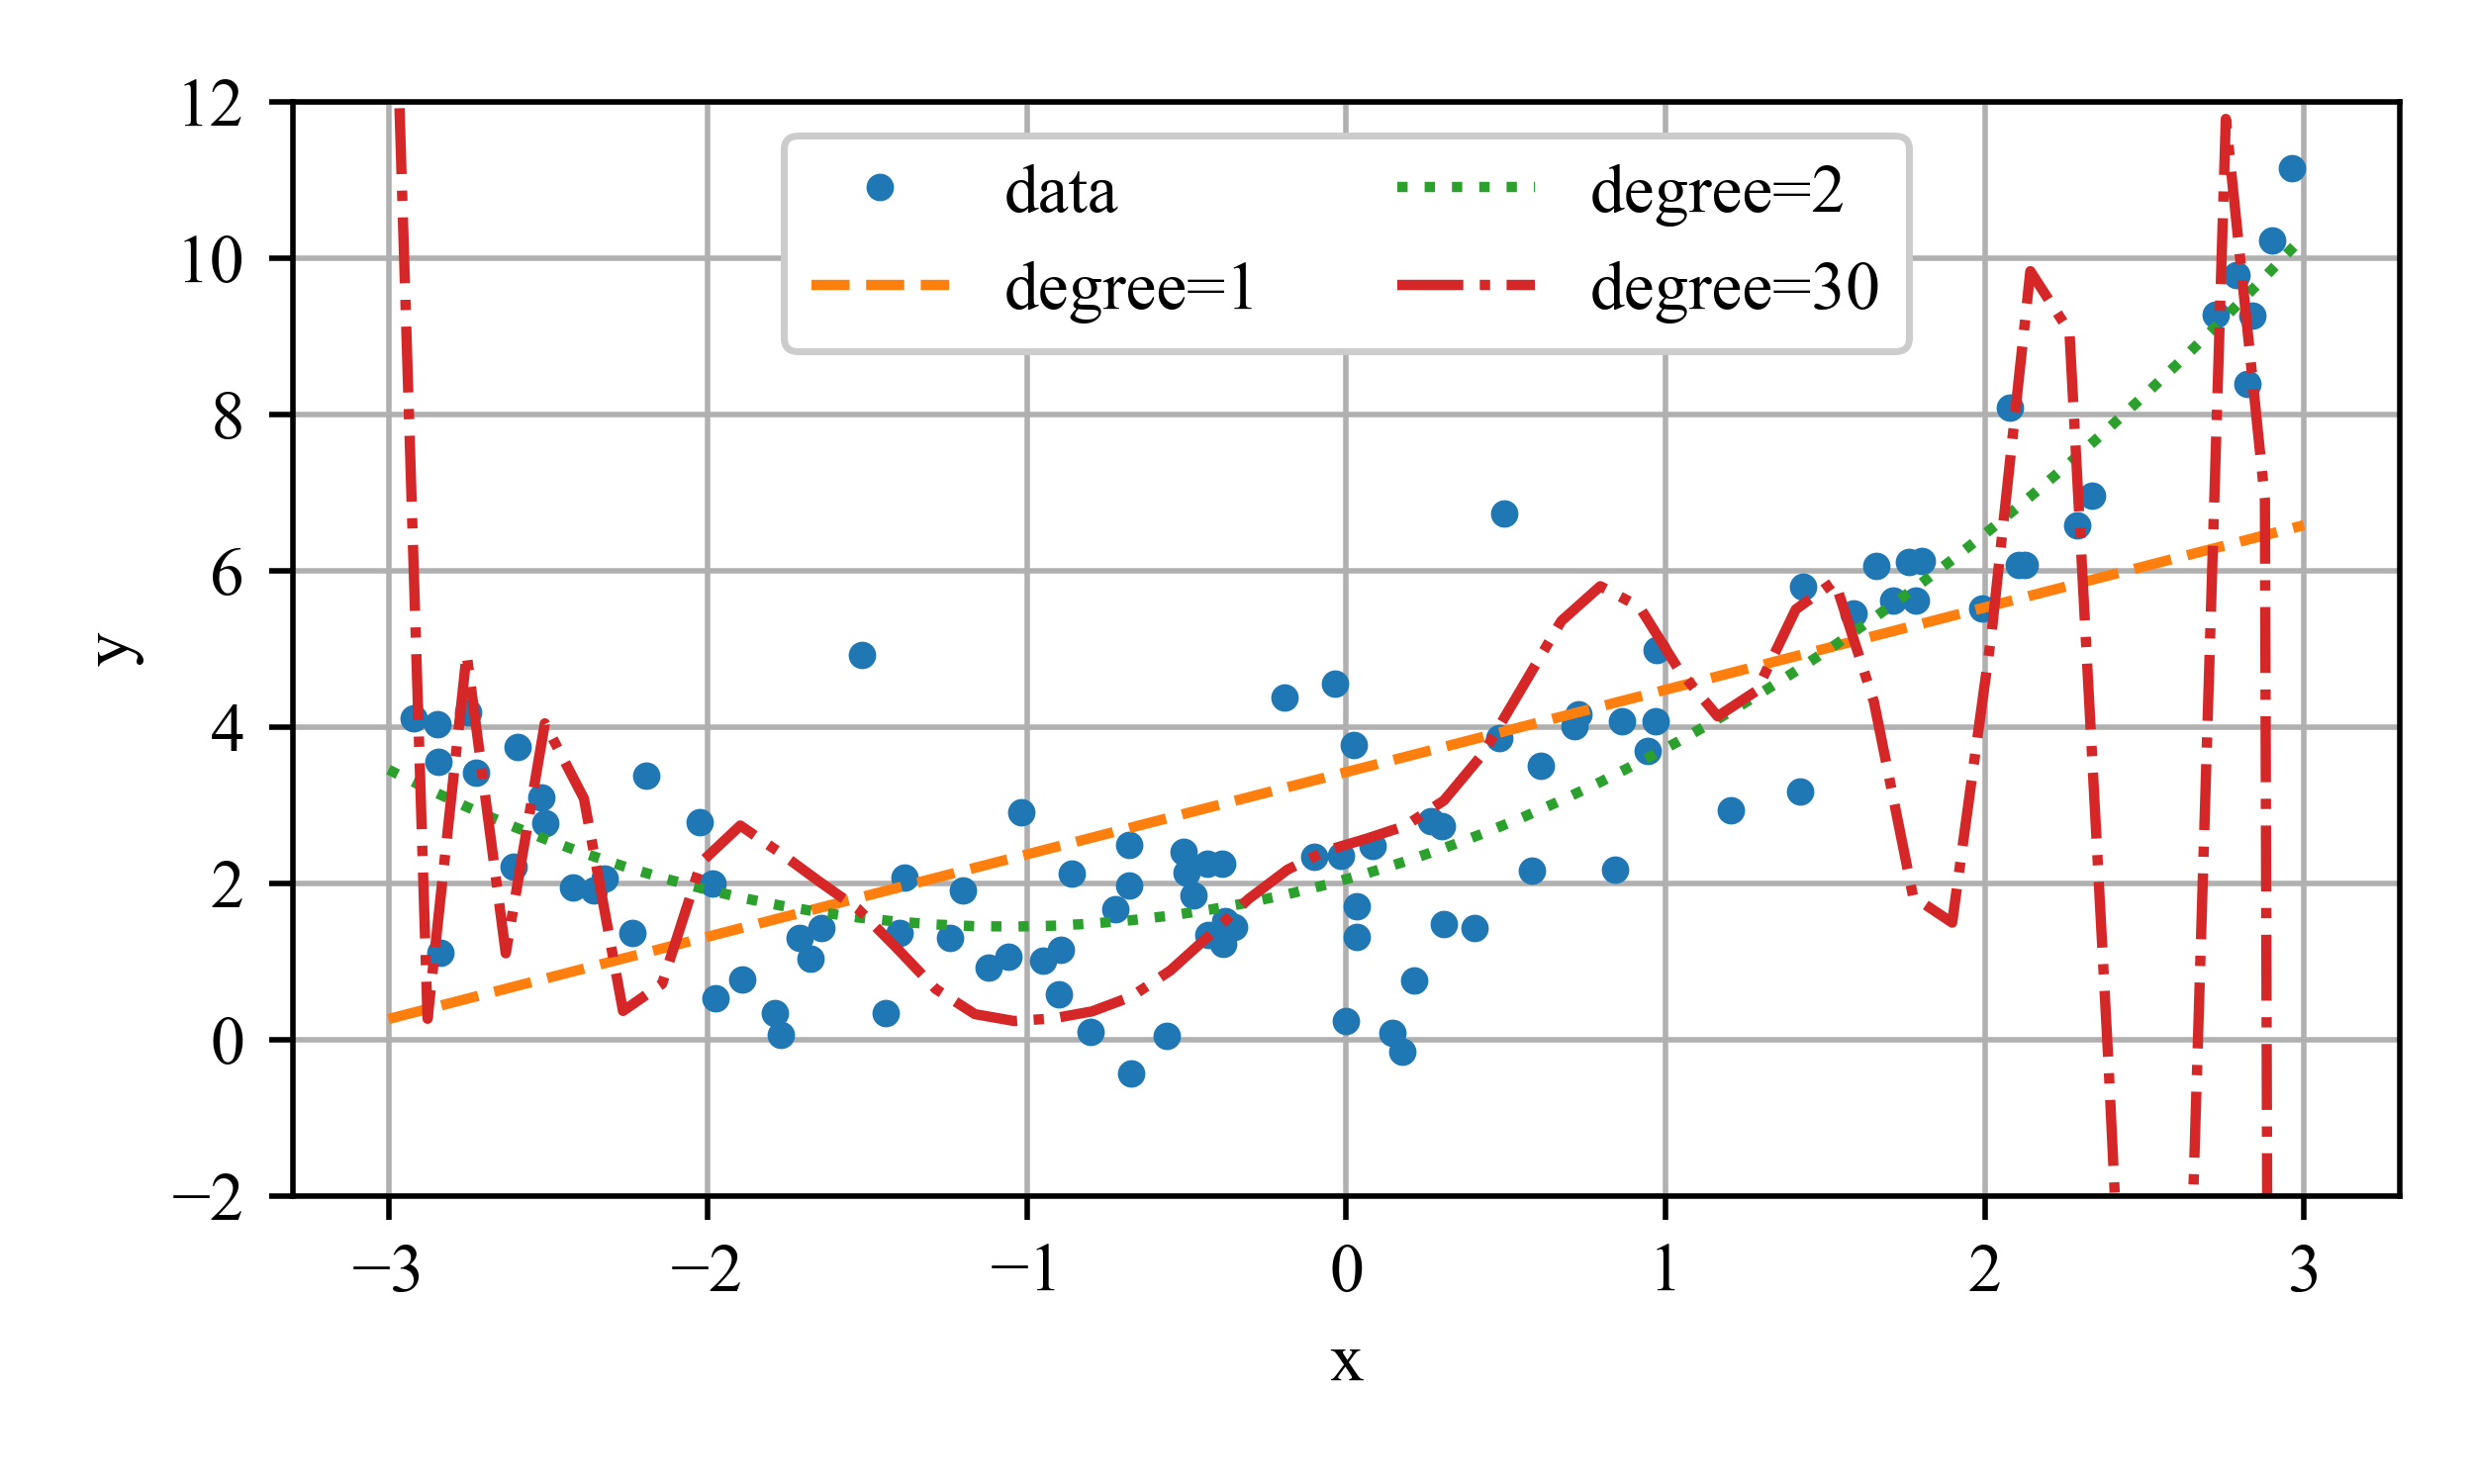
\includegraphics[]{../figures/overfitting_1.png}
\caption{Polynomial regression showing underfitting (degree=1), a respectable model fit (degree=2), and overfitting (degree=30).}
\label{fig:overfitting_1}
\end{figure}





\begin{figure}[H]
\centering
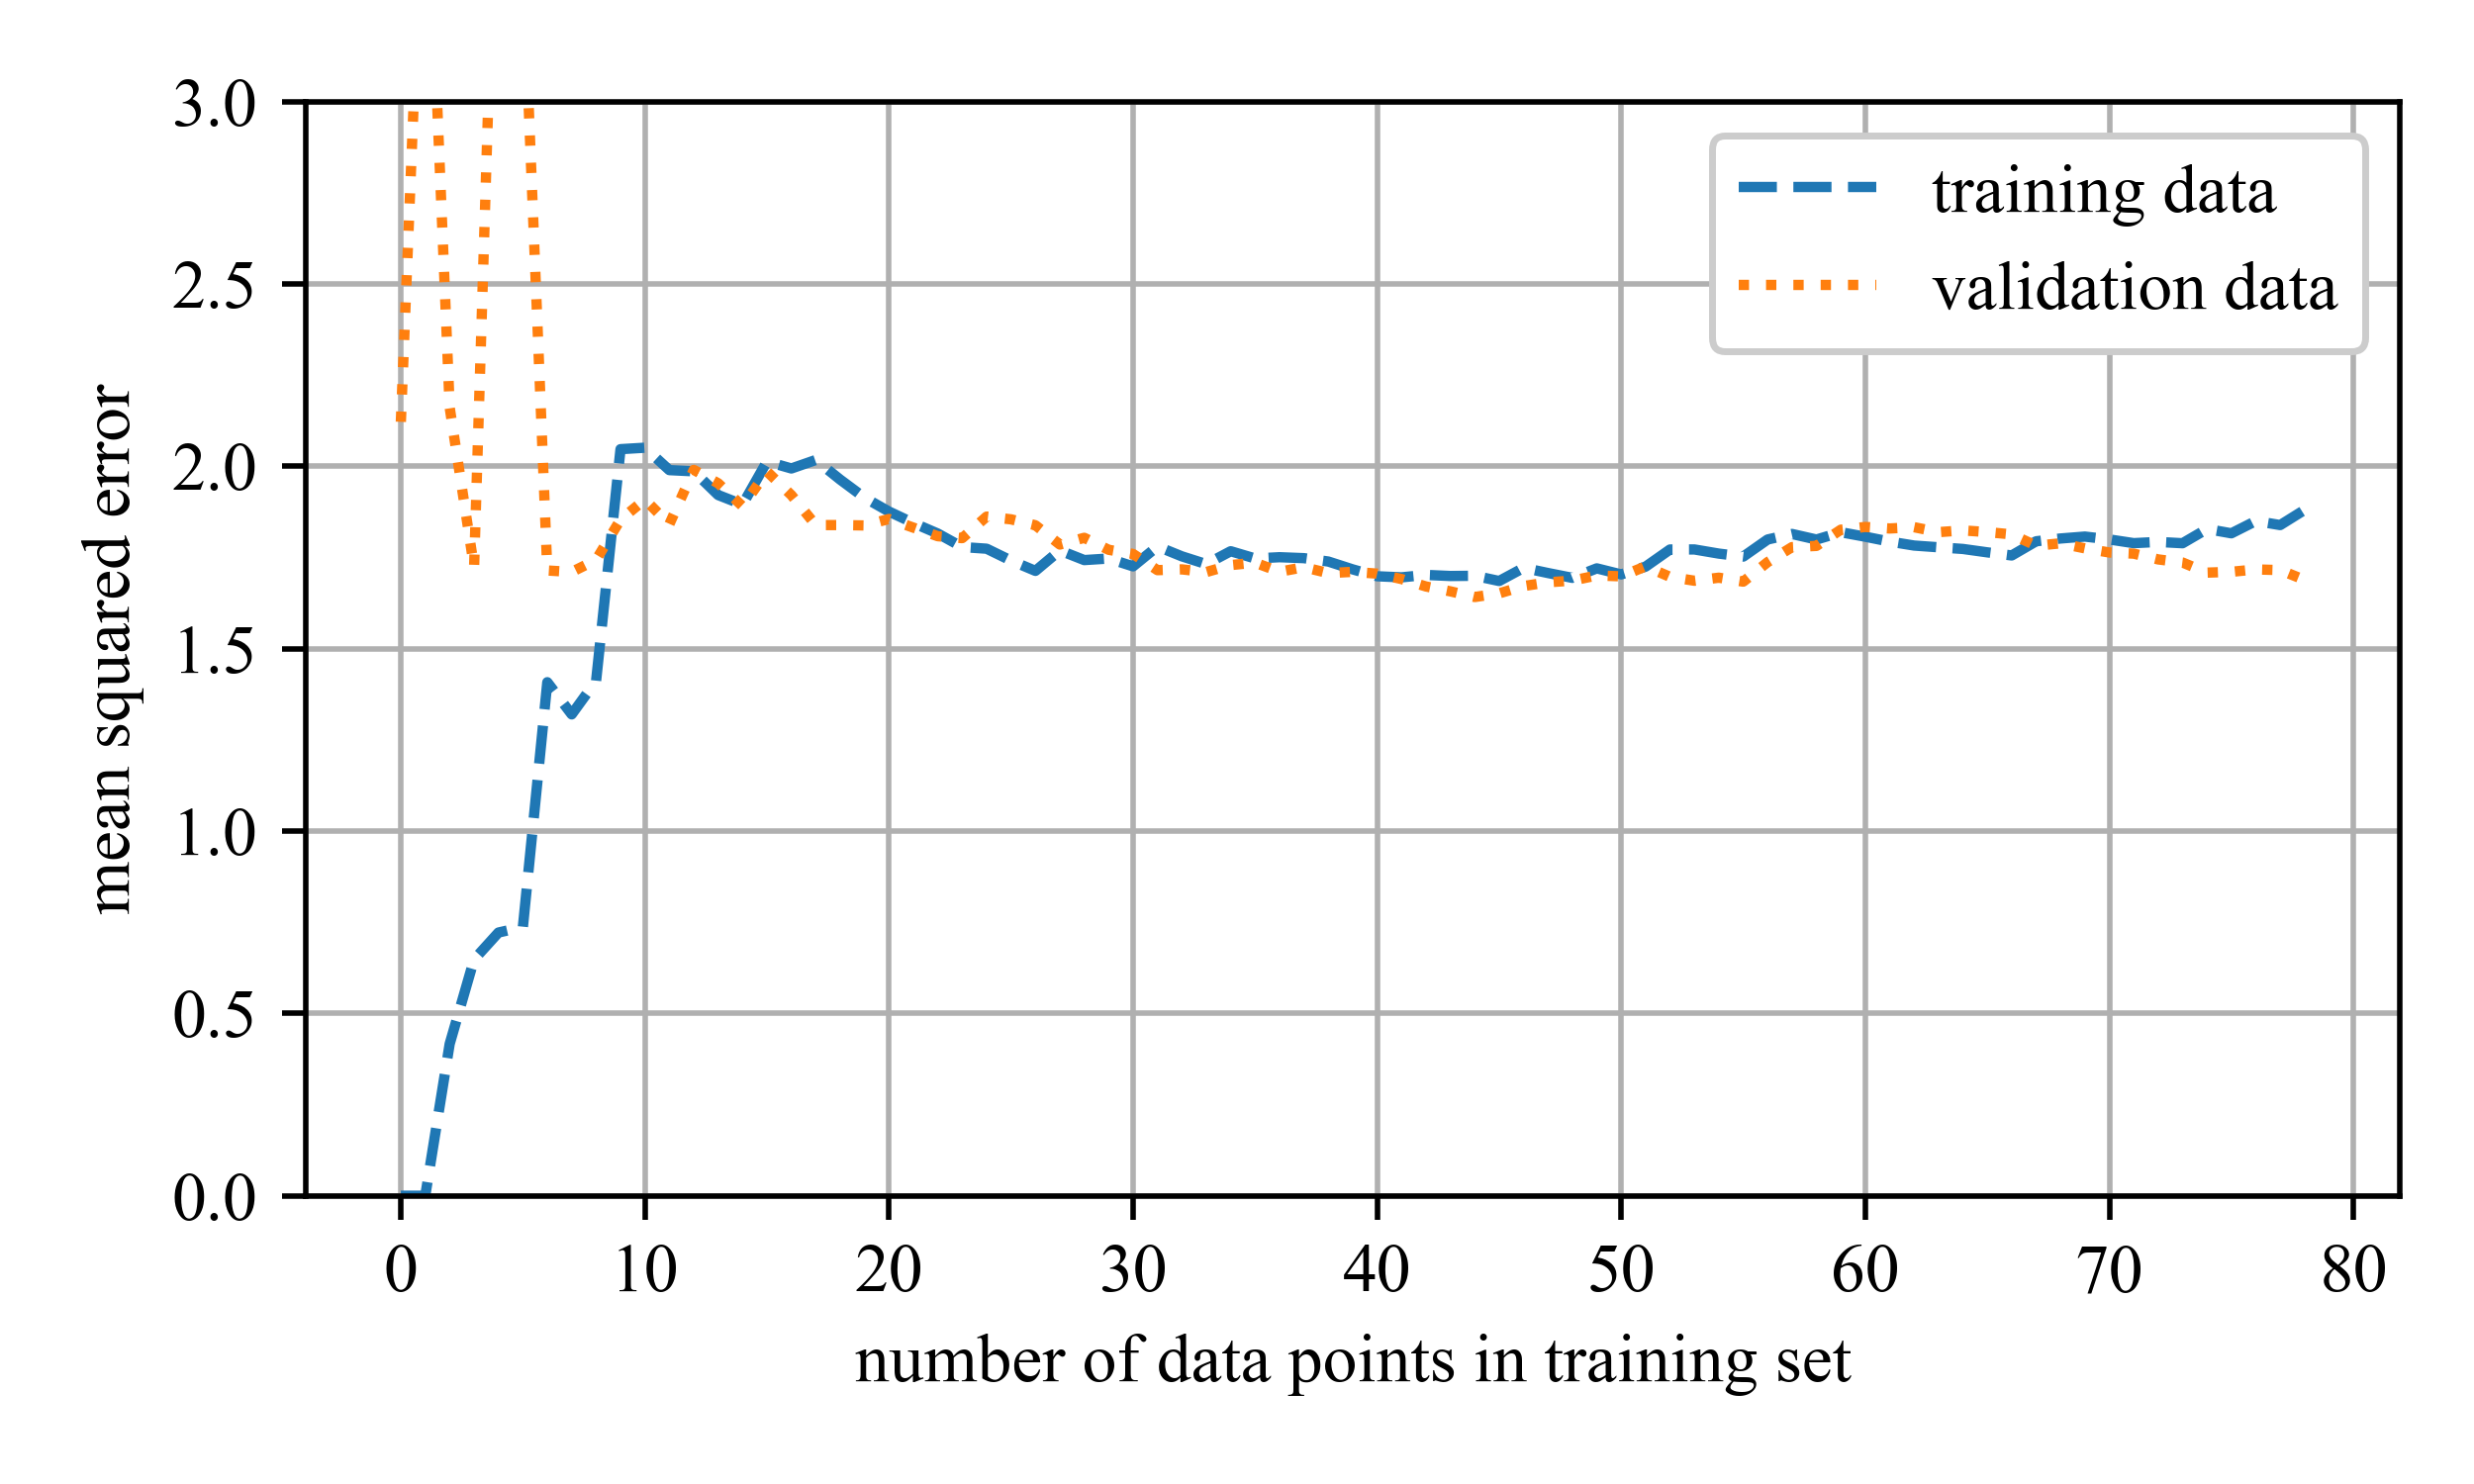
\includegraphics[]{../figures/overfitting_2.png}
\caption{Learning curves for the underfitting linear model (degree=1) where underfitting is evident because both curves have plateaued; they are close together and relatively high.}
\label{fig:overfitting_2}
\end{figure}

Examining the model's behavior in figures~\ref{fig:overfitting_2}~and~~\ref{fig:overfitting_3} on the training set shows a clear trend. With only one or two samples the fit is perfect, so the error curve begins at zero. As additional observations are introduced the model can no longer capture every point exactly, partly because of measurement noise and partly because the underlying relationship is nonlinear, and consequently the training error rises. After a sufficient number of samples the curve flattens out; beyond this plateau adding further data neither markedly lowers nor raises the average error.

\begin{figure}[H]
    \centering
    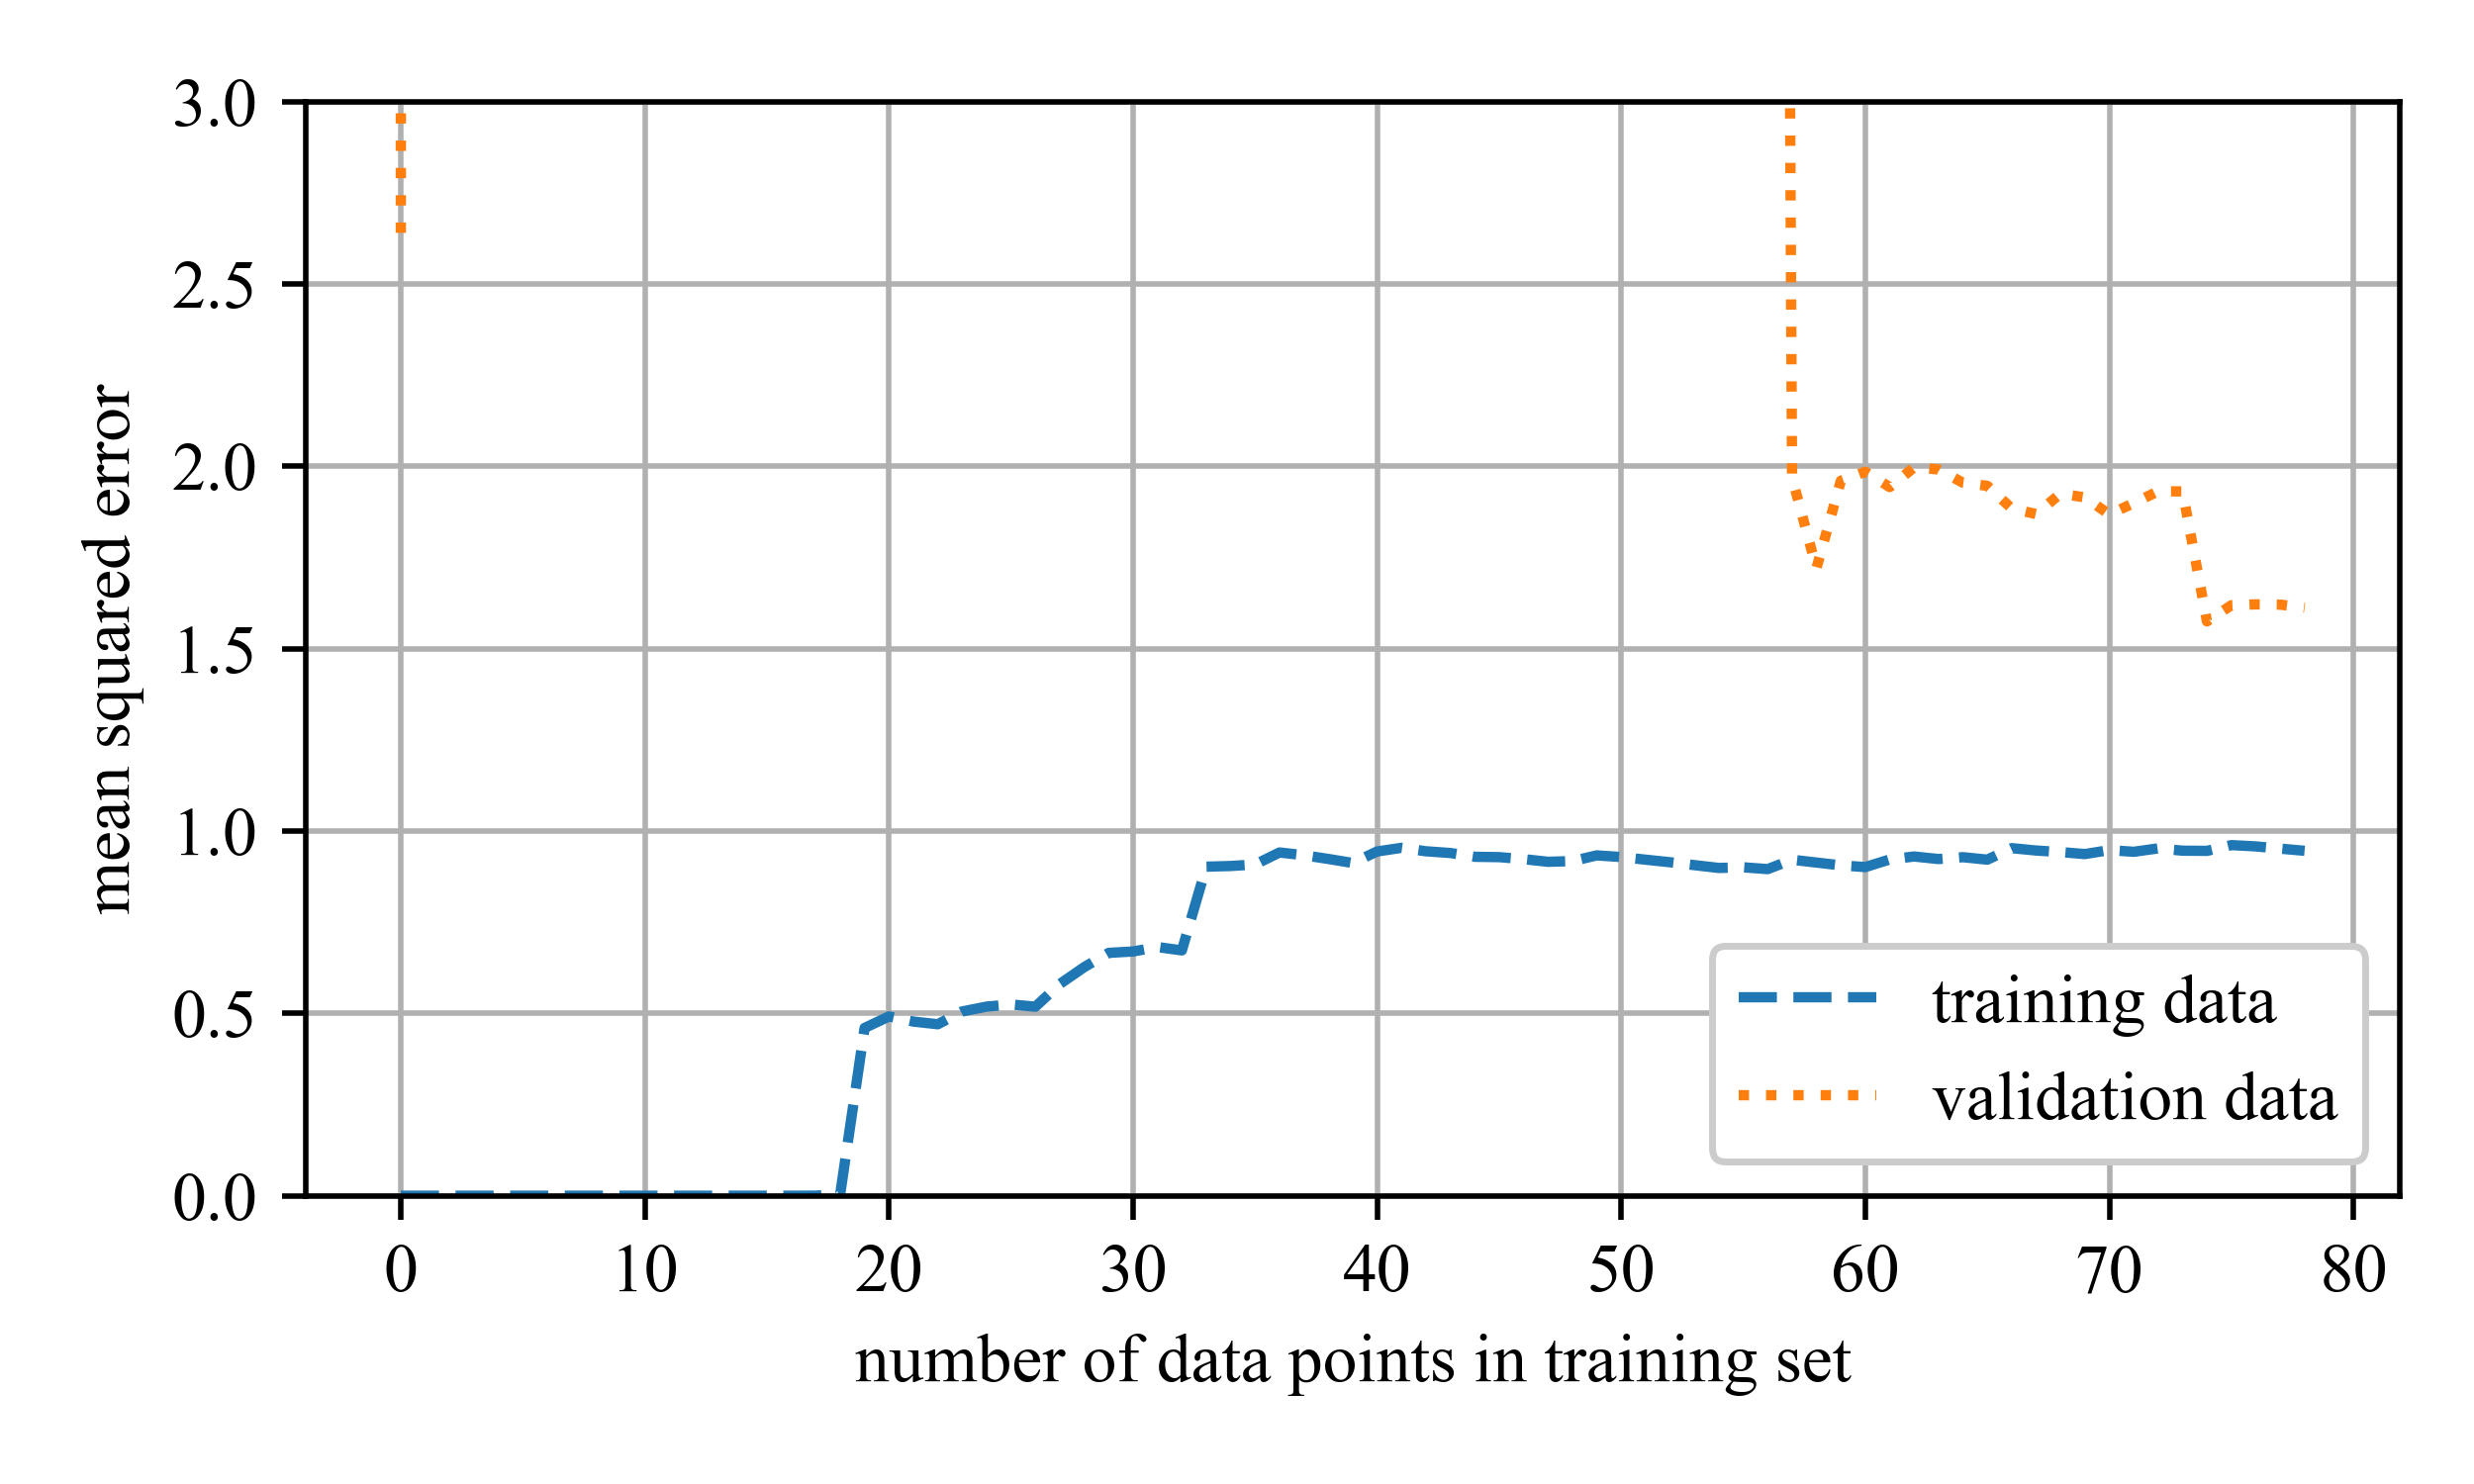
\includegraphics[]{../figures/overfitting_3.png}
    \caption{Learning curves for the overfitting polynomial model (degree=20) showing a significant gap between the curves, which indicates better performance on the training data than on the validation data.}
    \label{fig:overfitting_3}
\end{figure}

Inspection of the validation curve in figure~\ref{fig:overfitting_3}  tells a complementary story. With only a handful of training samples the model cannot generalize, so the validation error starts high. As more examples become available it learns progressively better patterns and the error falls. Eventually, though, the simple linear hypothesis is unable to capture the data's full complexity, causing the decline to flatten out; the validation curve plateaus at nearly the same level as the training curve. Their close proximity and uniformly large values are characteristic of an underfitting model.


Figure~\ref{fig:overfitting_3} displays the learning curves for a model fitted with a 20\textsuperscript{th}-degree polynomial. The overall shape resembles the curves seen earlier, yet two key differences stand out. First, the error on the training set is far lower than that achieved by the Linear Regression model, demonstrating the polynomial's extra flexibility. Second, a pronounced gap separates the training and validation curves, which means the model performs much better on the data it has already seen; this divergence is the hallmark of overfitting. Expanding the training set could reduce the gap, but without additional regularization the risk of overfitting would remain.


Next, let's apply the code using a 2\textsuperscript{nd} order polynomial, which accurately captures the essence of the data without underfitting or overfitting. These results are shown in Figure~\ref{fig:overfitting_4}. Here it can be seen that the training and validation curves again meet after converging, showing a well-fit model.

\begin{figure}[H]
    \centering
    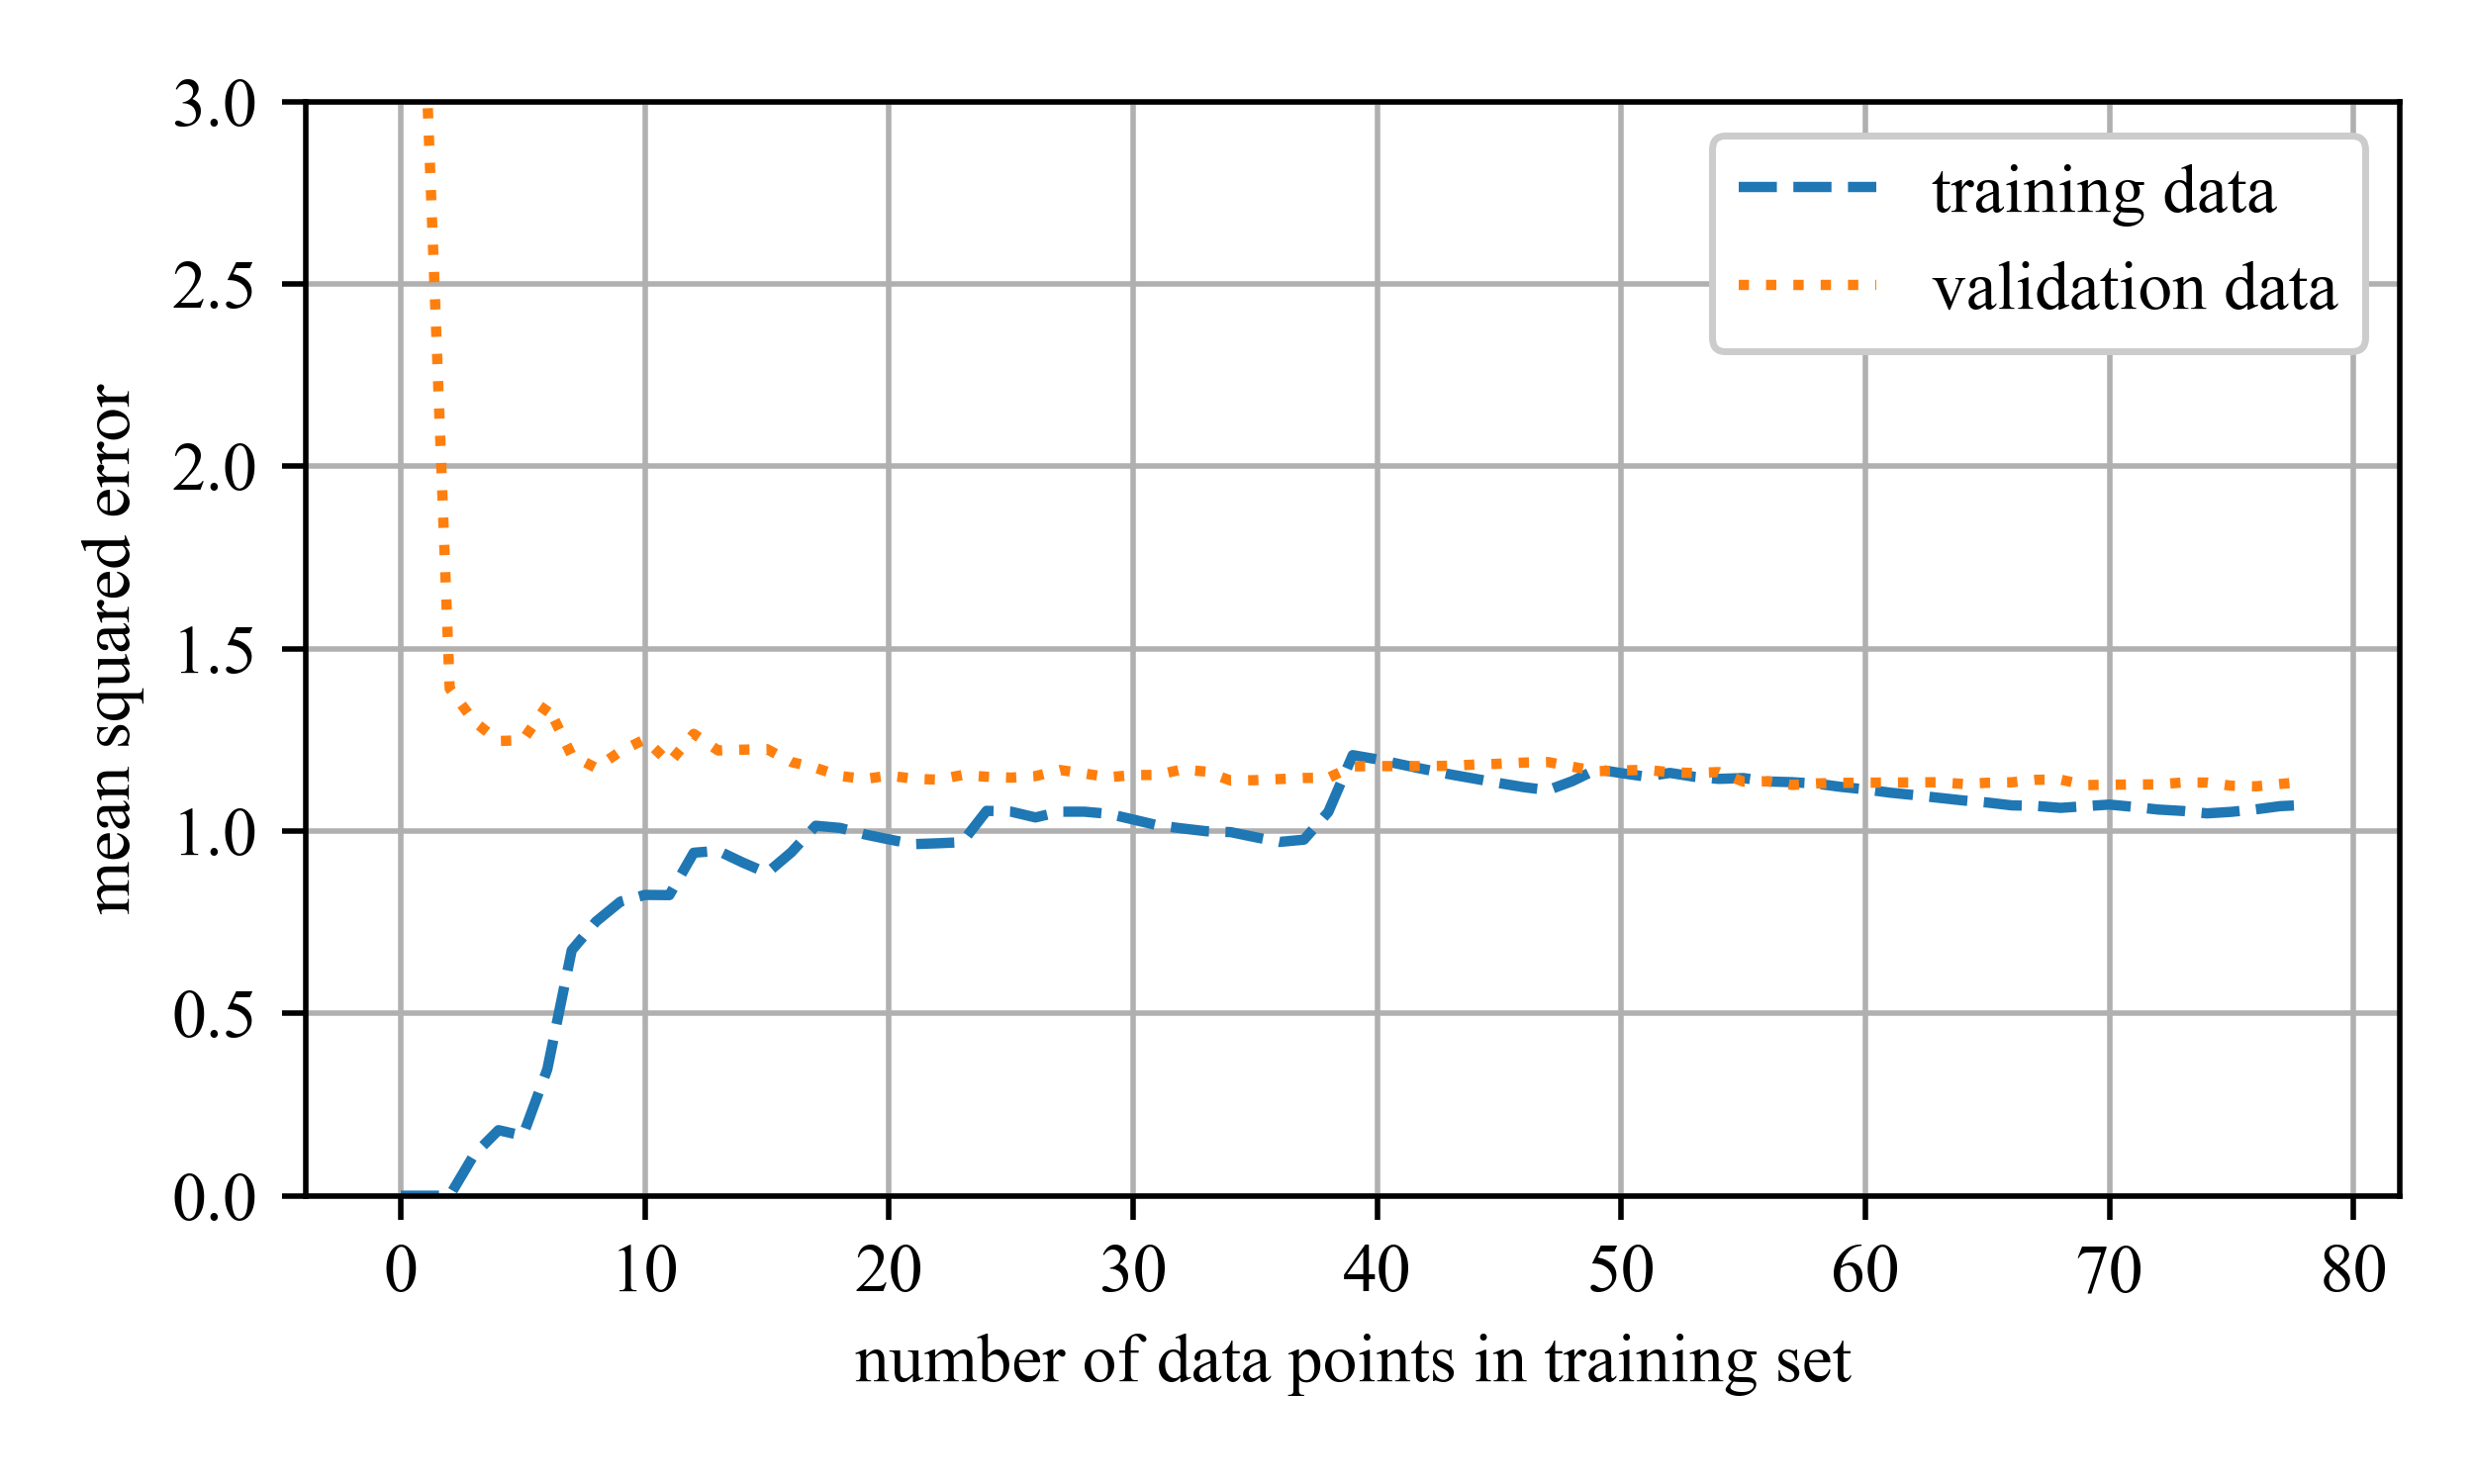
\includegraphics[]{../figures/overfitting_4.png}
    \caption{Learning curves for the optimal polynomial model (degree=2) showing well-aligned curves that plateau at a relatively low error level.}
    \label{fig:overfitting_4}
\end{figure}



\begin{example}
\textbf{Learning Curves}

\noindent This example compares learning curves for linear and polynomial regression models. By plotting training and validation errors as the training set grows, it illustrates how model complexity impacts bias and variance, and helps identify underfitting and overfitting behavior.
\end{example}




\subsection{Regularized Linear Models}
Overfitting is frequently curbed by regularizing the model, meaning you introduce constraints that reduce its effective degrees of freedom and make it harder to memories noise. In a polynomial setting you can achieve this simply by choosing a lower-degree polynomial, while in a linear model you typically add a penalty that discourages large coefficient values. This naturally raises the question: how is regularization expressed mathematically?


\subsubsection{Ridge Regression}

% \todo{Clarify the benefits of ridge regression and refine the description.}



Ridge Regression modifies Linear Regression by adding a regularization term to the cost function, which compels the learning algorithm to fit the data while keeping the model weights as small as possible. The updated cost-function is
\begin{equation}
J(\theta) = \text{MSE}(\theta) + \alpha \frac{1}{2} \sum_{i=1}^{n} \theta_i^2.
\label{eq:ridge_regression}
\end{equation}
The hyperparameter $\alpha$ dictates the degree of regularization. If $\alpha = 0$, Ridge Regression reduces to plain Linear Regression. If $\alpha$ is very high, the model weights are significantly shrunk, resulting in a nearly flat line through the mean of the data. Equation~\ref{eq:ridge_regression} outlines the cost function for Ridge Regression. The bias term $\theta_0$ is not regularized, as indicated by the summation starting from $i = 1$.

\begin{mdframed}[middlelinewidth=0.5mm]
\begin{center}
\bl{NOTE}
\end{center}
The regularization term is only included during the training phase. After training, the model's performance should be evaluated based on the unregularized performance measure.
\end{mdframed}

\begin{figure}[H]
    \centering
    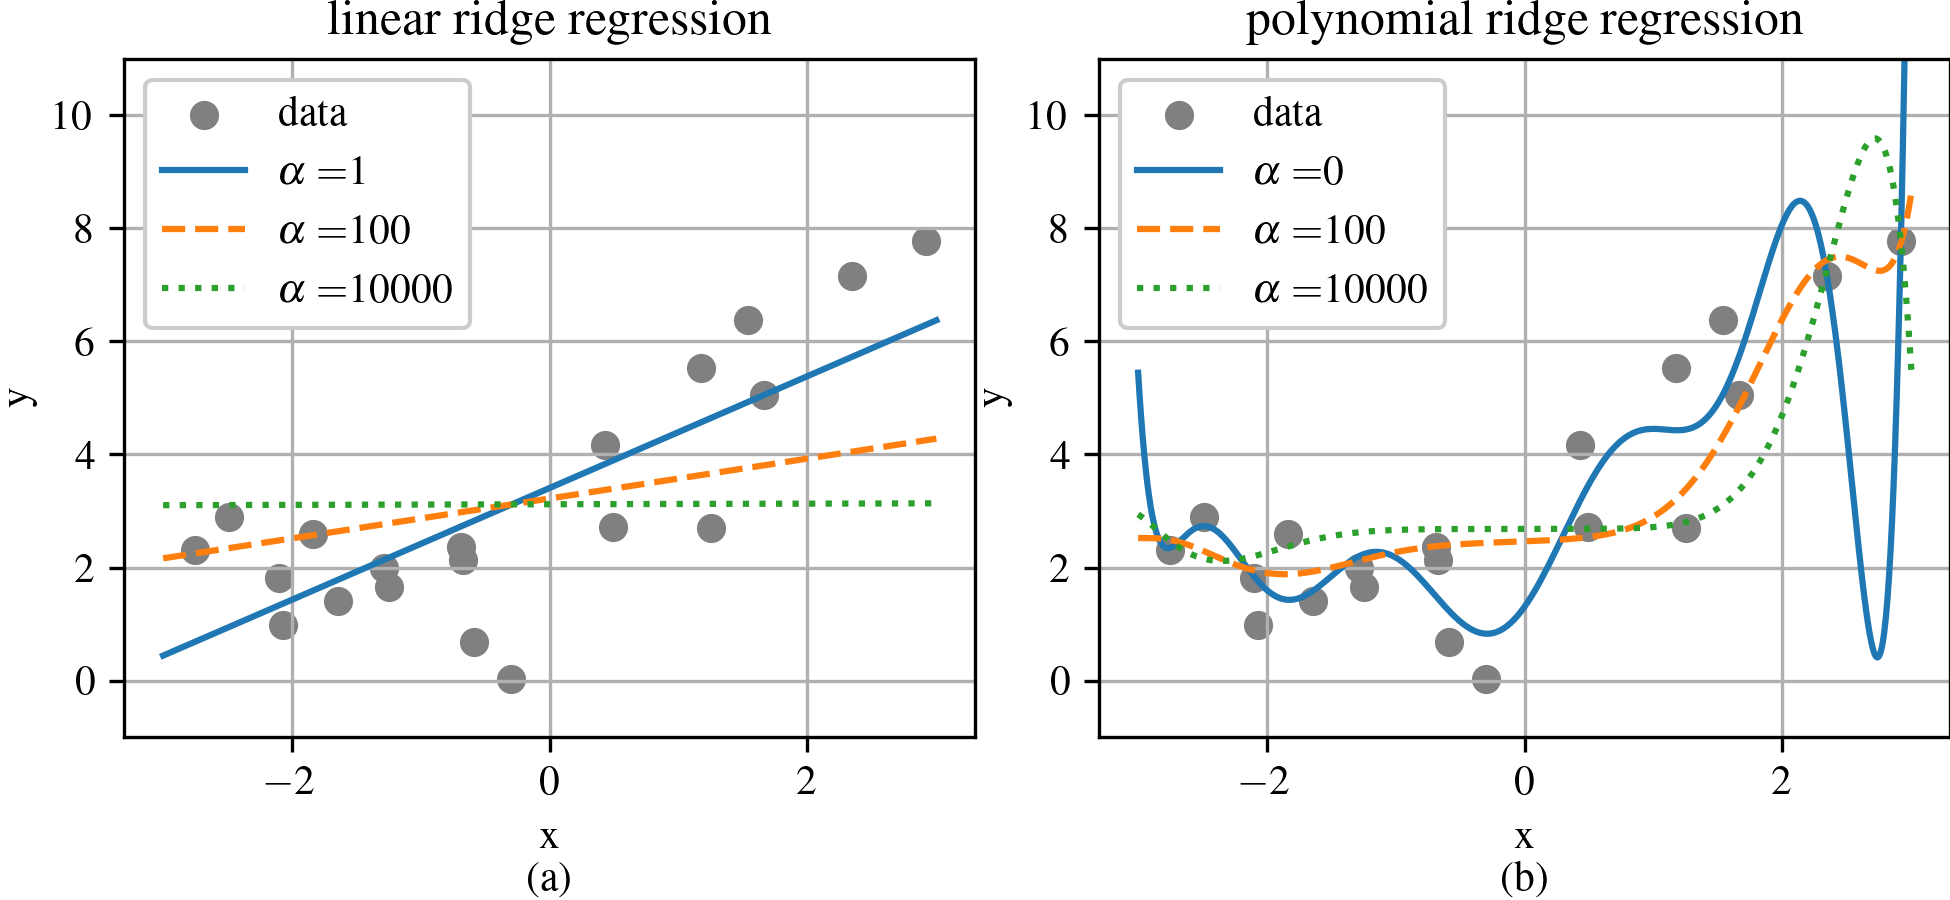
\includegraphics[width=6.5in]{../figures/ridge_regression.png}
    \caption{Visualization of Ridge Regression models with varying $\alpha$ values.}
    \label{fig:ridge_regression}
\end{figure}

Figure~\ref{fig:ridge_regression} illustrates various Ridge models trained on linear data, showcasing different $\alpha$ value. In Figure~\ref{fig:ridge_regression}(a), models are purely Ridge Regression, leading to linear predictions. In Figure~\ref{fig:ridge_regression}(b), the data undergoes Polynomial Regression with Ridge regularization. To do this, the data is first expanded using \texttt{PolynomialFeatures(degree=10)}, then scaled with \texttt{StandardScaler}, and finally, Ridge models are applied to these transformed features.


Increasing $\alpha$ results in flatter (i.e., more reasonable and less extreme) predictions, thereby reducing the model's variance but increasing its bias. Ridge Regression can be performed using a closed-form solution or through Gradient Descent, similar to Linear Regression. The pros and cons for each method mirror those discussed previously. The closed-form solution, an extension of the normal equation, is given by:
\begin{equation}
\hat{\theta} = (X^\text{T} \cdot X + \alpha A)^{-1} \cdot X^\text{T} \cdot y
\end{equation}
where $\alpha$ influences the regularization and $A$ is an $n \times n$ identity matrix with the top-left value replaced by 0 to exclude the bias term. When using Gradient Descent, the derivative of the cost function guides the adjustment toward optimal model parameters.

\begin{example}
\textbf{Ridge Regression}

\noindent This example demonstrates Ridge Regression as a regularized alternative to linear regression. A high-degree polynomial model is fit to noisy data using a pipeline with Ridge regularization, showing how the regularization term reduces overfitting and stabilizes the model.
\end{example}


%\subsubsection{Lasso Regression}
%
%\rd{Discuses other types of regularization.}
%
%
%
%\subsubsection{Elastic Net}
%
%\rd{Discuses other types of regularization.}

\subsection{Early Stopping}

An alternative approach to regularizing iterative learning methods 
(such as Gradient Descent) is to halt training as soon as the validation error hits its lowest point, a strategy known as early stopping. Figure~\ref{fig:early_stopping} illustrates a complex model, specifically a high-degree Polynomial Regression model, being refined through Batch Gradient Descent. Over the course of training, as epochs progress, the model's prediction error (RMSE) on both the training and validation sets decreases. However, after some time, the validation error ceases to decline and begins to increase, signaling that the model is beginning to overfit the training data. By implementing early stopping, training is terminated the moment the validation error reaches its minimum. Geoffrey Hinton praised this method stating, ``Early stopping (is) beautiful free lunch'' due to its simplicity \protect\footnotemark[1].

\footnotetext[1]{Pennington, Jeffrey, Richard Socher, and Christopher D. Manning. ``Glove: Global vectors for word representation.'' Proceedings of the 2014 conference on empirical methods in natural language processing (EMNLP). 2014.}


		\begin{figure}[H]
			\centering
			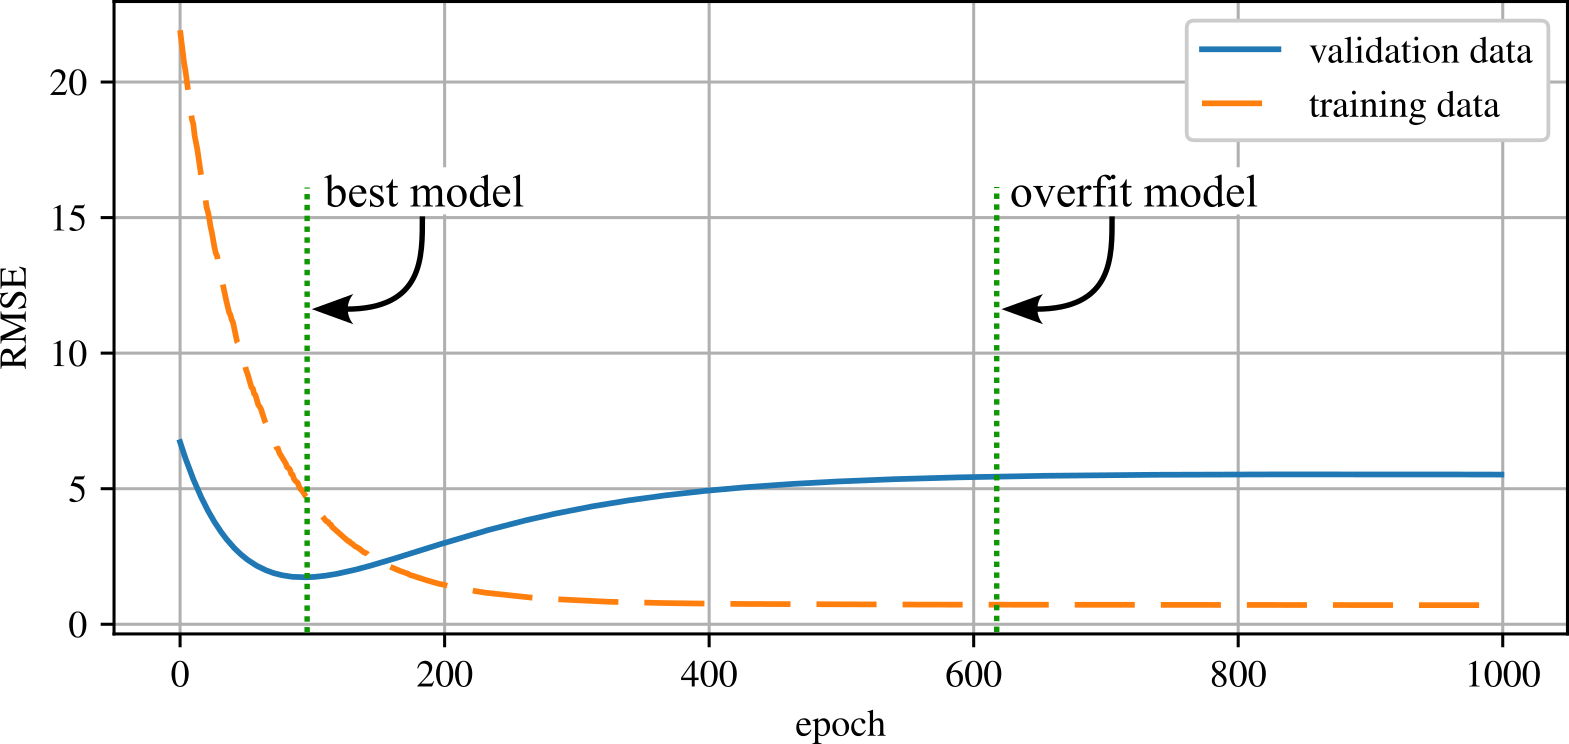
\includegraphics[width=6in]{../figures/early_stopping.png}
			\caption{An example showing how early stopping can result in a better model as it does not allow for the over-fitting of the training set.}
			\label{fig:early_stopping}
		\end{figure}


\begin{example}
\textbf{Early Stopping}

\noindent This example uses a high-degree polynomial model trained with stochastic gradient descent to demonstrate early stopping. By tracking training and validation errors across epochs, it highlights how halting training early can prevent overfitting and improve generalization.
\end{example}


\pagebreak
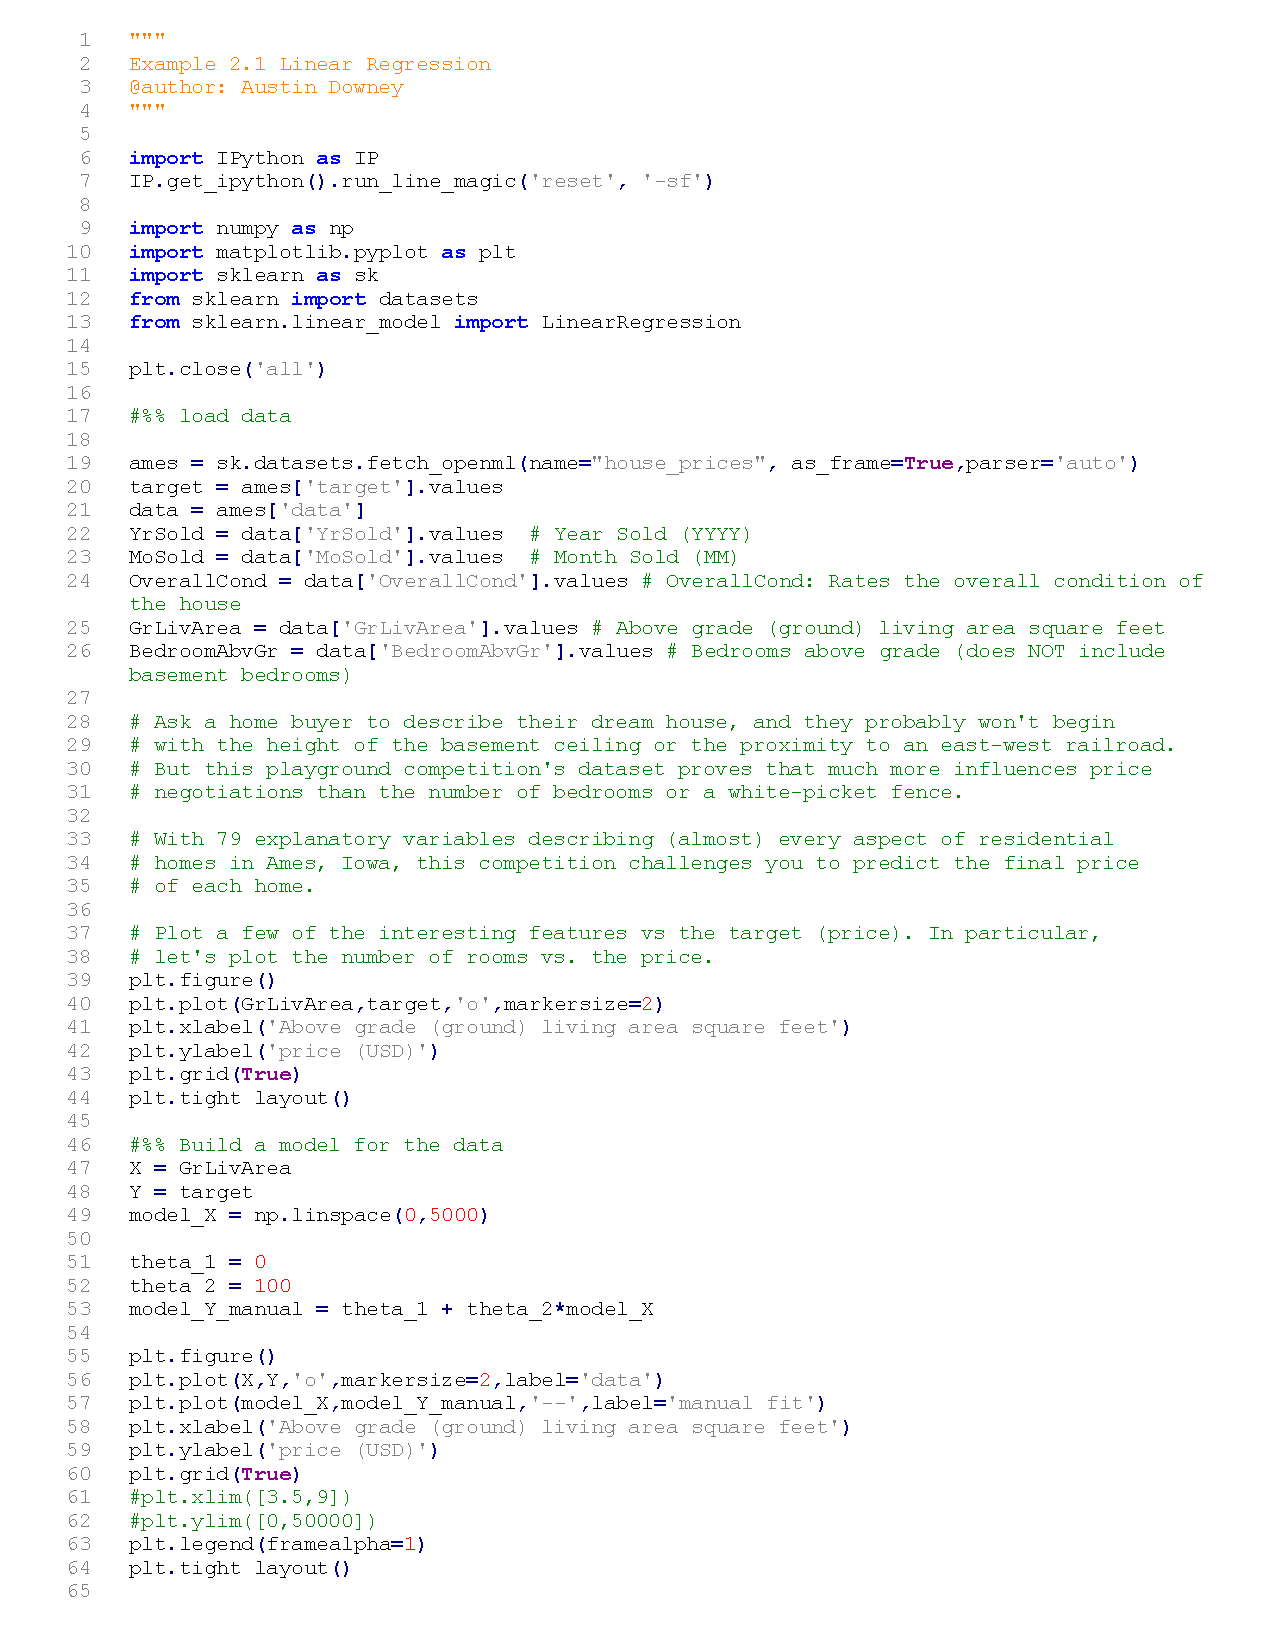
\includepdf[pages=1, width= 0.95\textwidth, pagecommand = {\subsection{Examples} \subsubsection*{Example 2.1}\vspace{0.5em}}]{../code/example_2.1_Ames_simple_linear_regression_model.pdf}
\includepdf[pages=2, width= 0.95\textwidth, pagecommand = {\vspace{0.5em}}]{../code/example_2.1_Ames_simple_linear_regression_model.pdf}
\includepdf[pages=3, width= 0.95\textwidth, pagecommand = {\vspace{0.5em}}]{../code/example_2.1_Ames_simple_linear_regression_model.pdf}

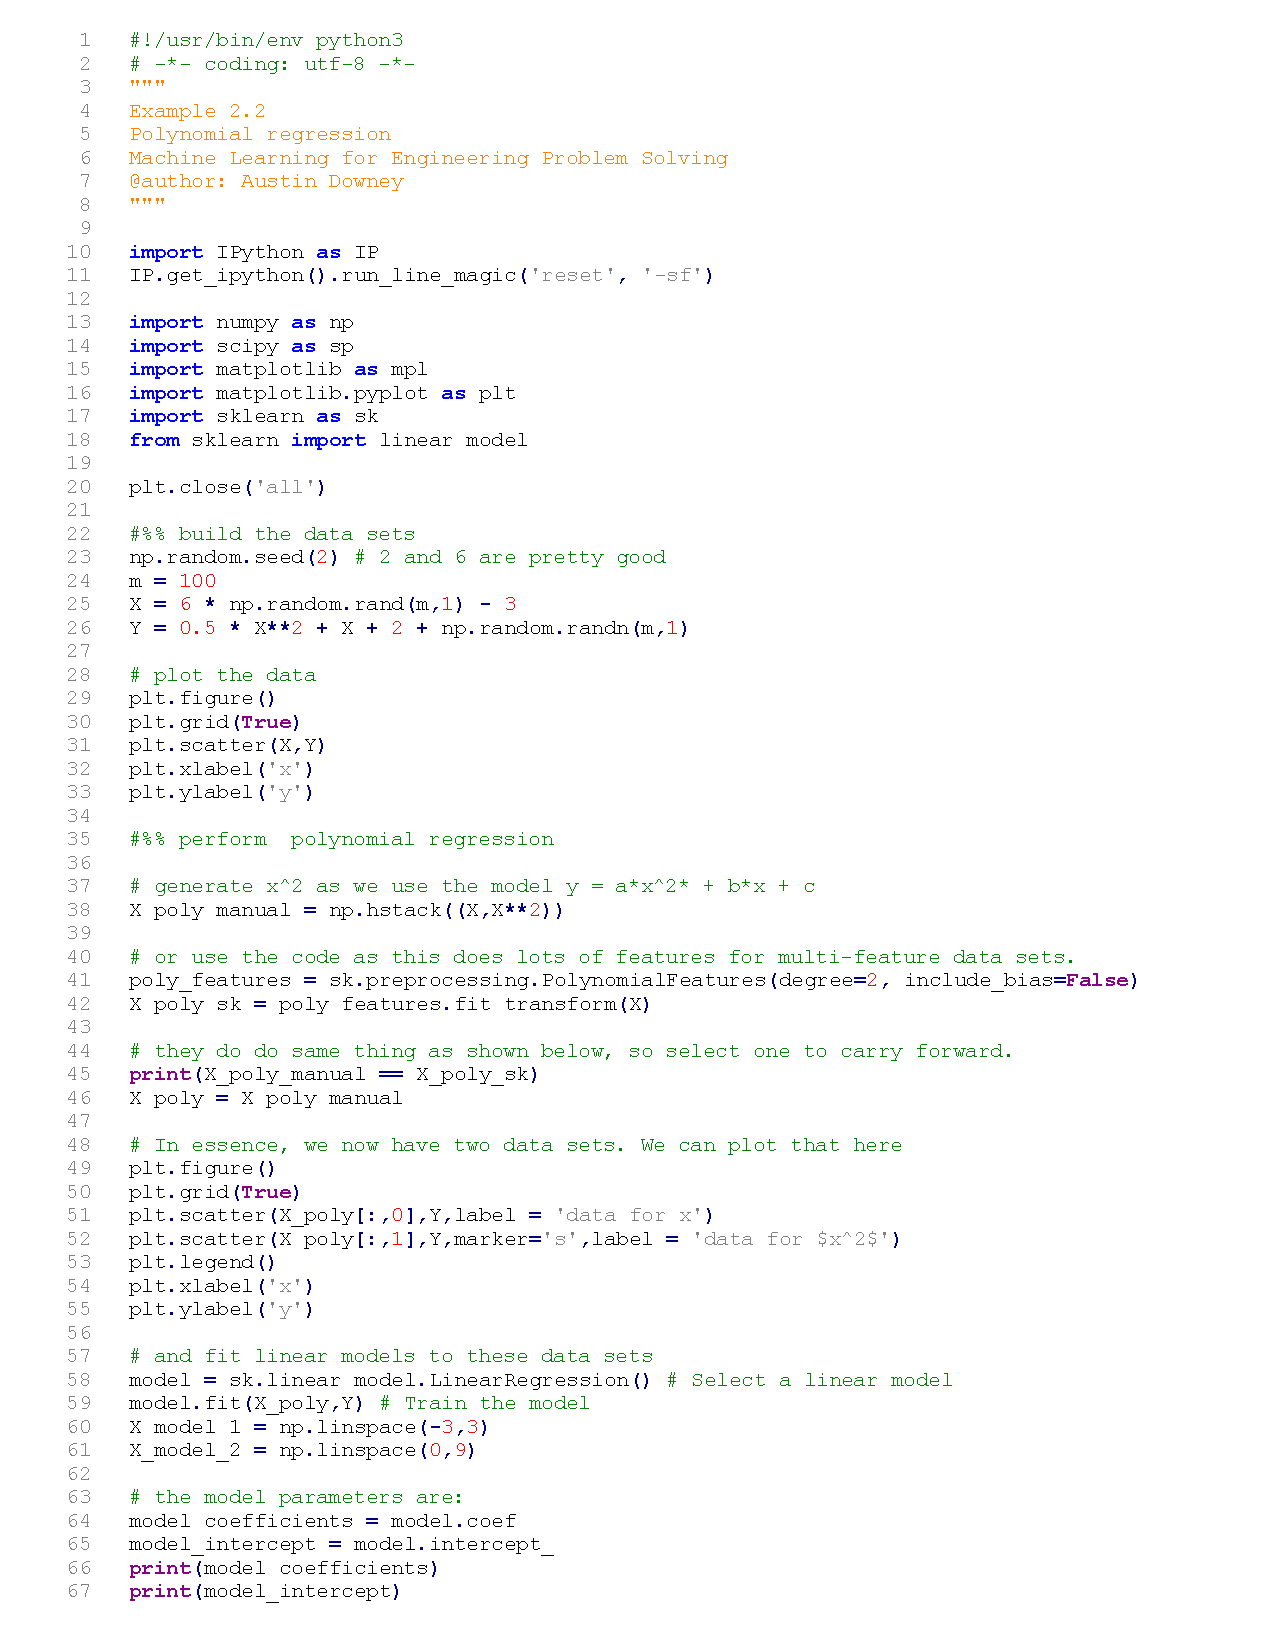
\includepdf[pages=1, width= 0.95\textwidth, pagecommand = {\subsubsection*{Example 2.2}\vspace{0.5em}}]{../code/example_2.2_polynominl_regression.pdf}
\includepdf[pages=2, width= 0.95\textwidth, pagecommand = {\vspace{0.5em}}]{../code/example_2.2_polynominl_regression.pdf}

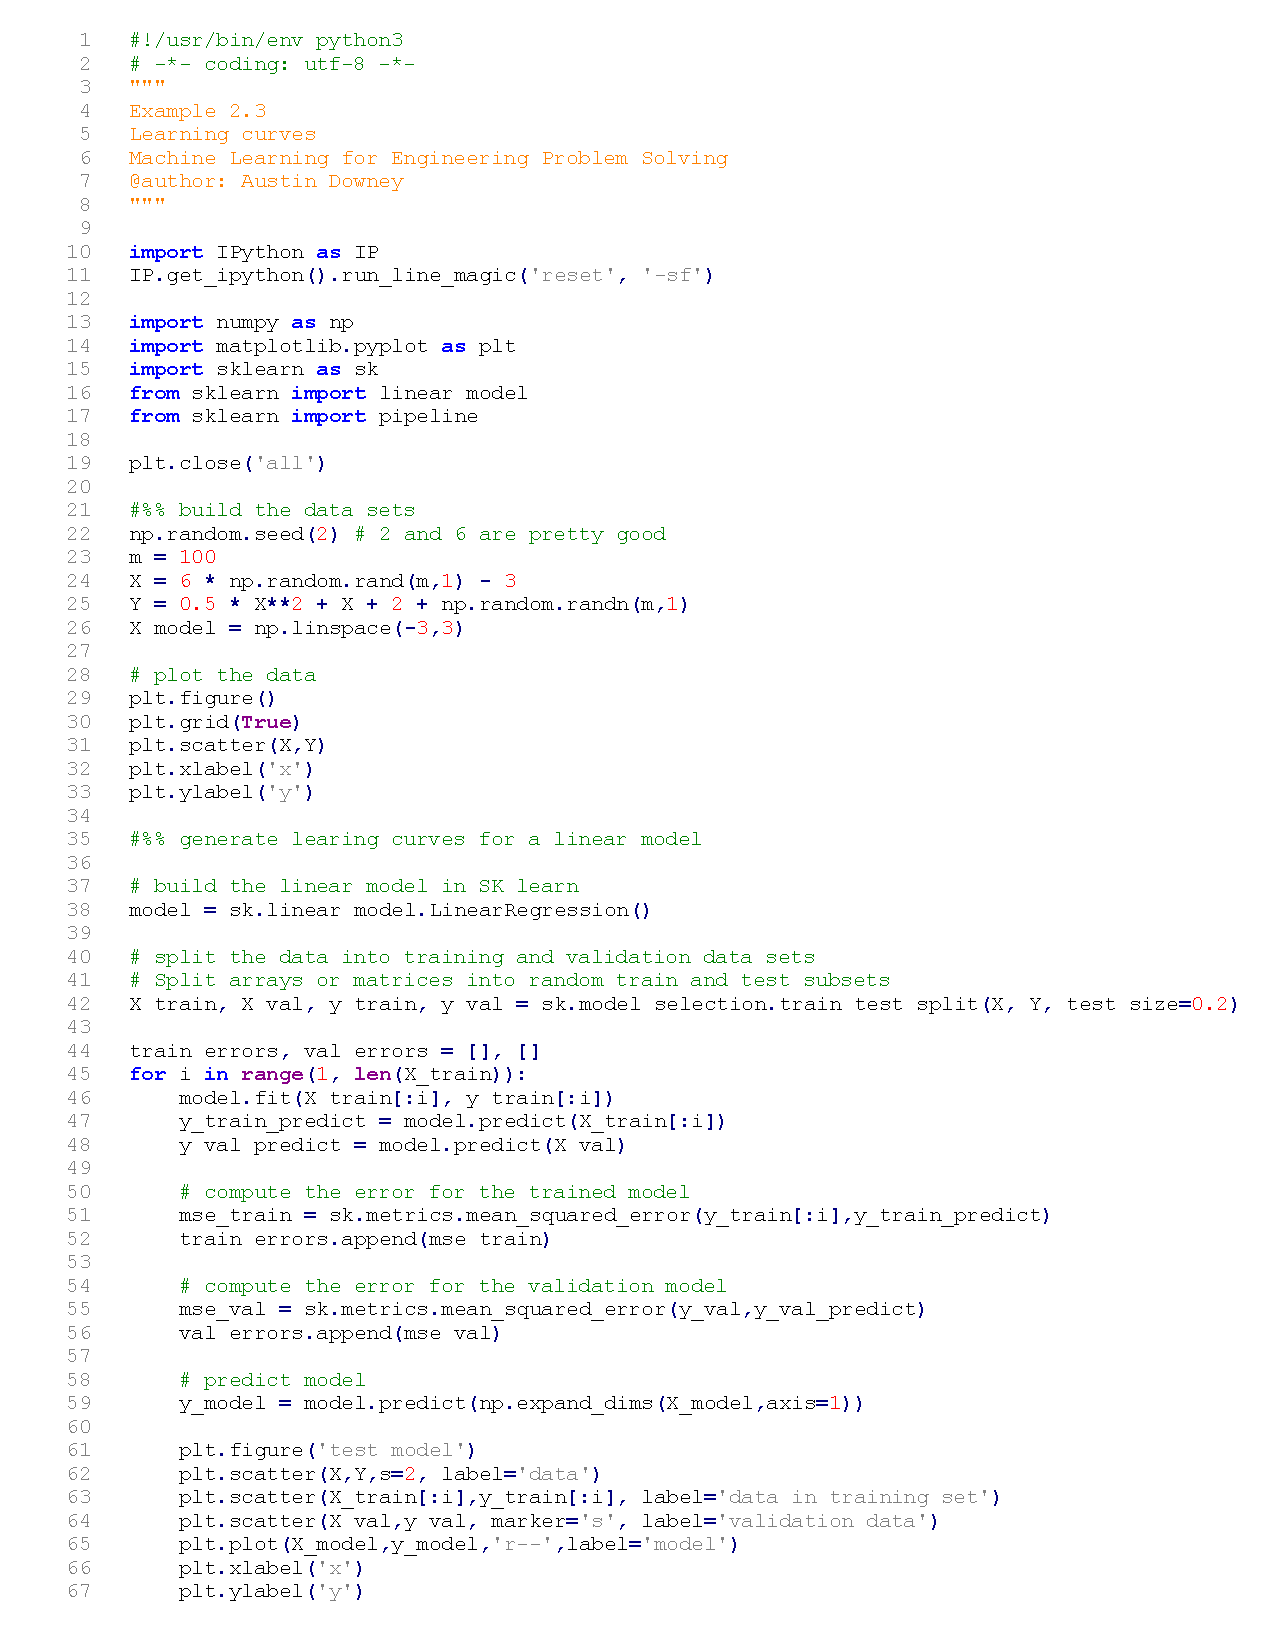
\includepdf[pages=1, width= 0.95\textwidth, pagecommand = {\subsubsection*{Example 2.3}\vspace{0.5em}}]{../code/example_2.3_learning_curves.pdf}
\includepdf[pages=2, width= 0.95\textwidth, pagecommand = {\vspace{0.5em}}]{../code/example_2.3_learning_curves.pdf}

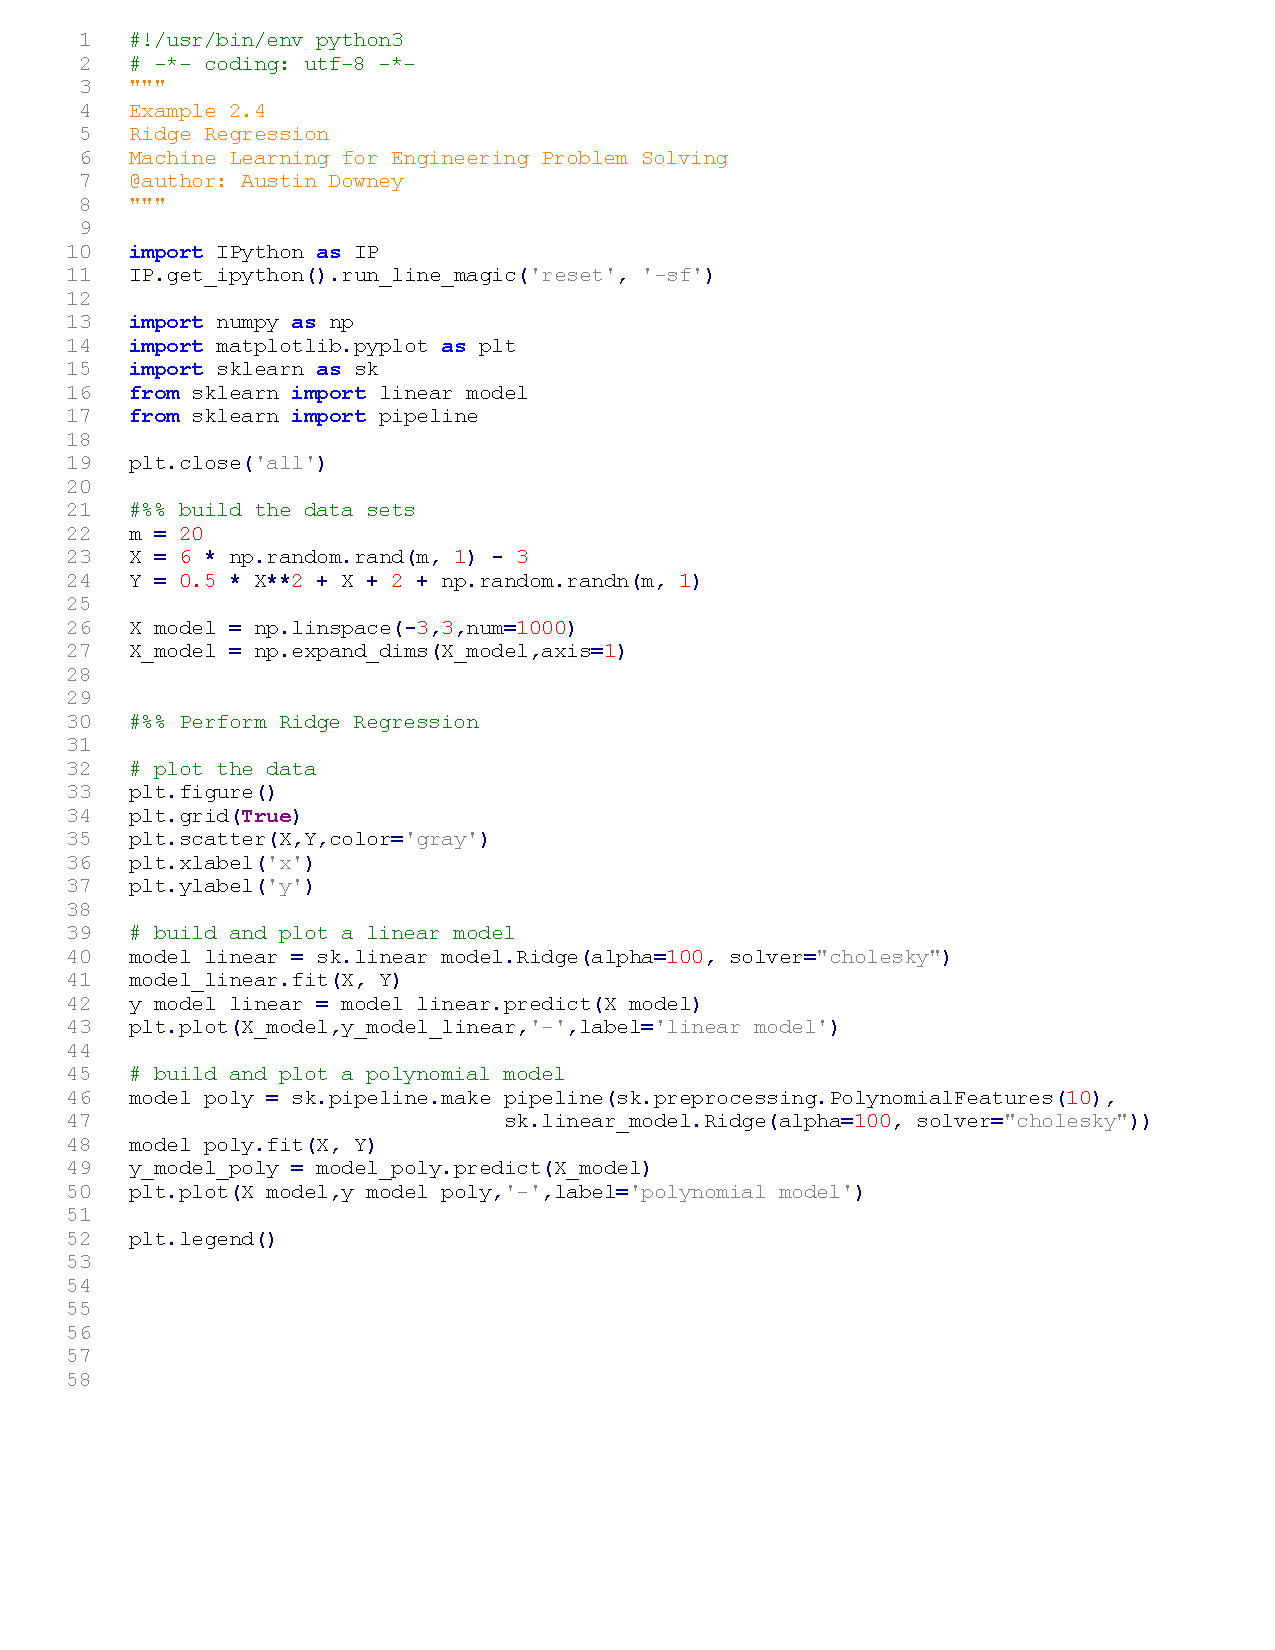
\includepdf[pages=-, width= 0.95\textwidth, pagecommand = {\subsubsection*{Example 2.4}\vspace{0.5em}}]{../code/example_2.4_ridge_regression.pdf}

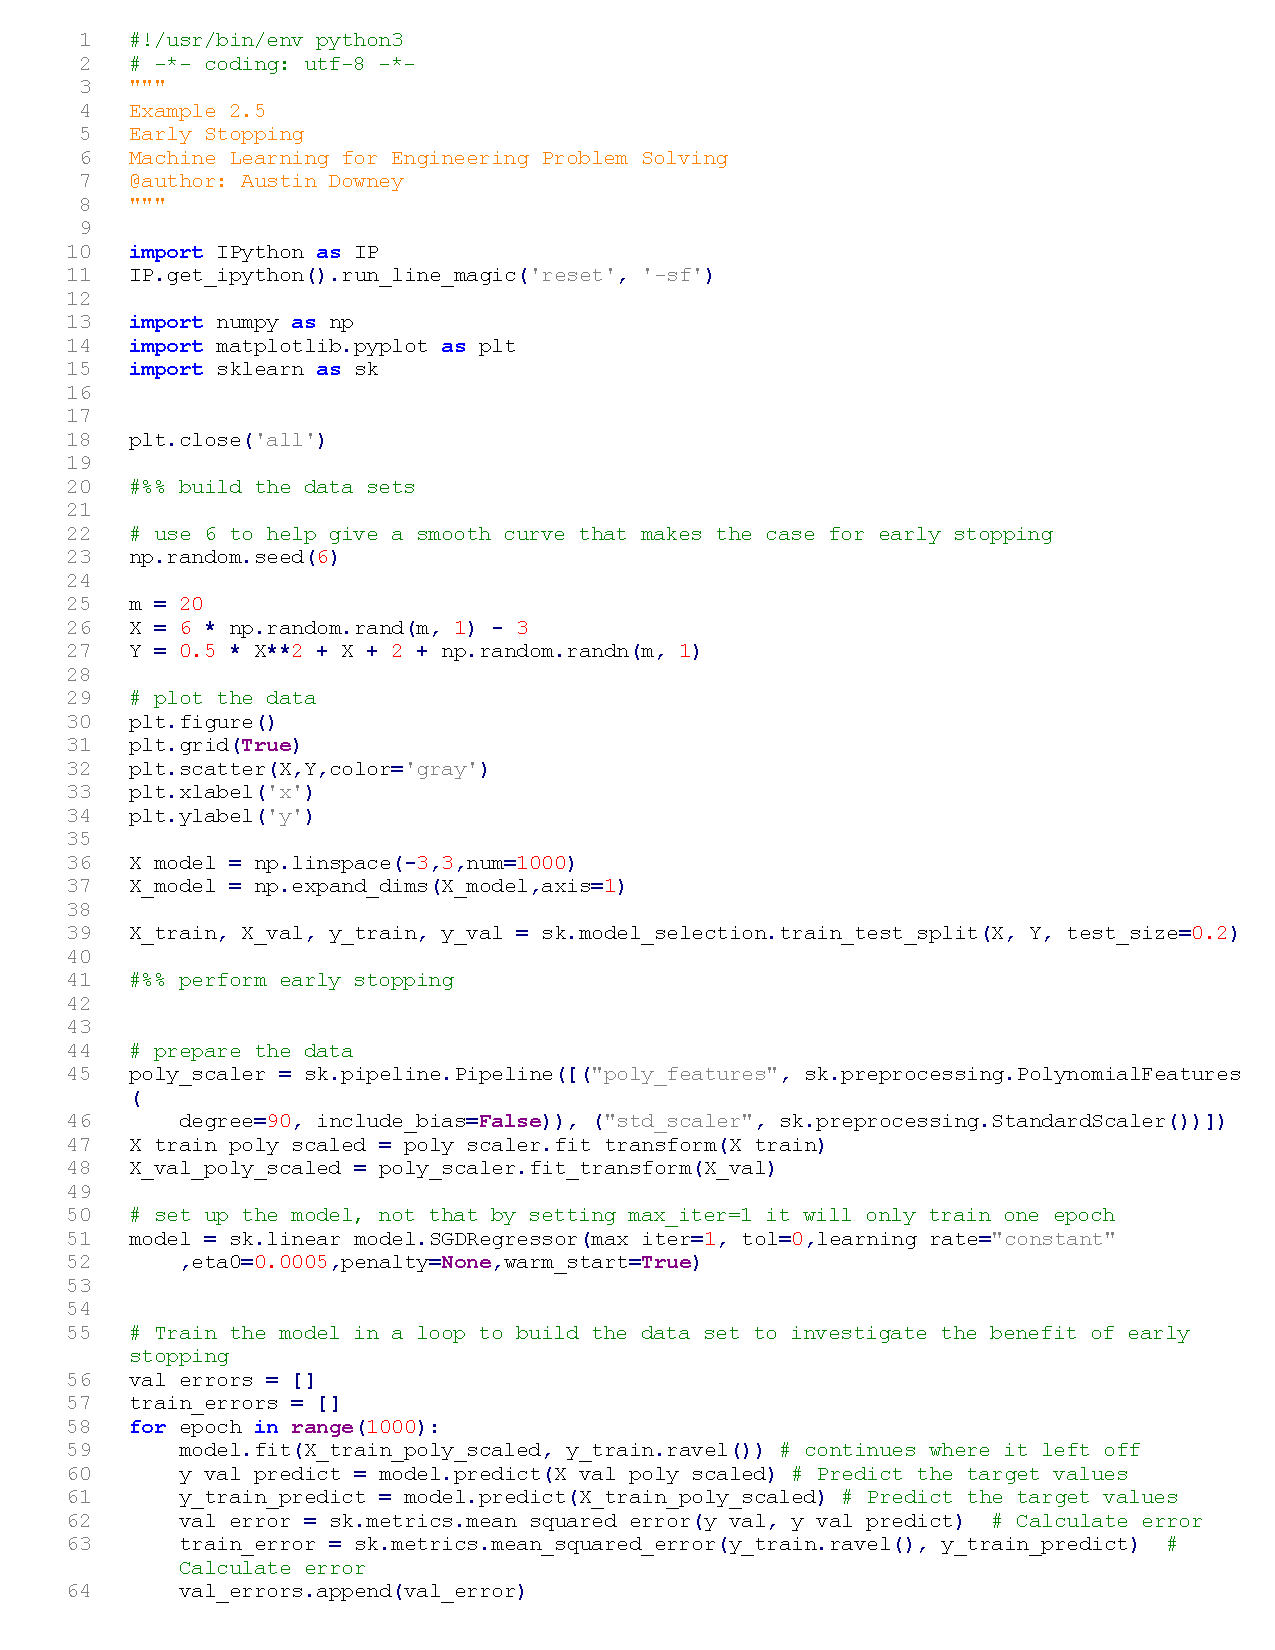
\includepdf[pages=1, width= 0.95\textwidth, pagecommand = {\subsubsection*{Example 2.5}\vspace{0.5em}}]{../code/example_2.5_early_stopping.pdf}
\includepdf[pages=2, width= 0.95\textwidth, pagecommand = {\vspace{0.5em}}]{../code/example_2.5_early_stopping.pdf}









\end{document}
